\documentclass[a4paper,11pt,twoside,pdftex]{article}

% Misc packages
\usepackage{float}
\usepackage{setspace} % for defining spacing between lines

% Package for nice printing of external config files and program code
\usepackage{listings} 
\lstset{basicstyle=\ttfamily\small,columns=fullflexible} %courier, non-aligned columns

% Allow colour for HTML links
\usepackage{color}
\definecolor{darkgray}{gray}{0.20}

% Geometery for A4 layout like MS-Word defaults
\usepackage[left=2.54cm,top=2.54cm,bottom=3.17cm,right=3.17cm]{geometry}

% Natlib to better cite references (round brackets, commas between refs, and sorted)
\usepackage[round,comma,sort]{natbib}

% hyperref for HTML links within pdf 
\usepackage{hyperref}  %EXAMPLE: \href{http://www.niwa.co.nz}{NIWA}
\hypersetup{
  breaklinks=true,      % allow line breaks in URLs
  colorlinks=true,      % use colour to define links
  linkcolor=black,      % colour of internal links
  citecolor=black,      % colour of links to bibliography
  filecolor=black,      % colour of file links
  urlcolor=darkgray     % colour of external links
}

% Making the index
\usepackage{makeidx}
\makeindex

% Graphics (no postscript files.. just use jpeg, png, etc)
\usepackage[dvips]{graphicx}
% Changes fonts to Times, Helvetica, Courier
\usepackage{pslatex} 

% Section header fonts
\usepackage{sectsty}
\allsectionsfont{\sffamily\large} % Normal sized arial style section headings
\makeatletter % this bit adds a 'dot' after the section head numbers
\def\@seccntformat#1{\csname the#1\endcsname.\quad}
\makeatother

% Page style
\usepackage{fancyhdr}
\pagestyle{fancy}
\fancyhead{}
\fancyfoot{}
\headheight 15pt
\renewcommand{\headrulewidth}{0pt} % rule line under header
\renewcommand{\footrulewidth}{0pt}
\setlength{\parindent}{0pt} % No indentation at start of paragraph
\setlength{\baselineskip}{1ex plus 0.2ex minus 0.1ex}
\setlength{\parskip}{\medskipamount} % Gap between paragraphs
\raggedbottom % prefer space at the bottom of page

%% stop figures from going onto a page by themselves 
\renewcommand{\topfraction}{0.85}
\renewcommand{\textfraction}{0.1}
\renewcommand{\floatpagefraction}{0.75}

%% make list gaps small
\newcommand{\denselist}{\itemsep 0pt\topsep-0.3ex\partopsep-0.3ex}

% New commands to define macros and other aids to text and layout
\newcommand{\config}{input configuration file}
\newcommand{\command}[1] {\texttt{@#1}}
\newcommand{\subcommand}[1] {\texttt{#1}}
\newcommand{\commandsub}[2] {\command{#1}\subcommand{#2}}
\newcommand{\argument}[1] {\texttt{#1}}

\newcommand{\commentline}{\#}
\newcommand{\commentstart}{\{}
\newcommand{\commentend}{\}}

\newcommand{\Rzero}{\emph{R}$_0$}
\newcommand{\Bzero}{\emph{B}$_0$}
\newcommand{\R}{\textbf{R}}

% New commands to template syntax definitions
% Define a command without a label
\newcommand{\defCom}[2]{\texttt{\textbf{@#1}} \hspace{0.5cm} {#2}}
% Define a command with a label
\newcommand{\defComLab}[2]{\texttt{\textbf{@#1}\ \emph{label}} \hspace{0.5cm} {#2}}
% Define a subcommand
\newcommand{\defSub}[2]{\texttt{#1} \hspace{0.5cm} #2 \\*}% Define a command with an argument
\newcommand{\defComArg}[3]{\texttt{\textbf{@#1}\ \emph{#2}} \hspace{0.5cm} {#3}}
% Define a Command\index{Command} argument
\newcommand{\defArg}[2]{\emph{\texttt{#1}} \hspace{0.5cm} #2 \\*}

% Generic definition for subcommand syntax 
\newcommand{\defText}[2]{\hangindent=0.3cm \small{#1\ #2}\normalsize \\*}
% Define subcommand syntax for Type / Default / Condition / Value / Note / Example
\newcommand{\defType}[1]{\defText{Type:}{#1}}
\newcommand{\defDefault}[1]{\defText{Default:}{#1}}
\newcommand{\defCondition}[1]{\defText{Condition:}{#1}}
\newcommand{\defValue}[1]{\defText{Value:}{#1}}
\newcommand{\defNote}[1]{\defText{Note:}{#1}}
\newcommand{\defExample}[1]{\defText{Example:}{#1}}

% Input SVN version definitions
%============================================================================
% svn_version : A command line utility to extract source control revision
%               number, date, and time.
% Author      : S.Rasmussen / A.Dunn
% Copyright   : Copyright NIWA (c)2008 - www.niwa.co.nz
%============================================================================

% Warning: This file is an atomatically generated file describing the source
% control revision number, date, and time using svn_version.

% Call: svn_version --format tex --recursive --quiet --suffix Doc 
% Current working directory: C:\Projects\General\SPM\doc\manual

\newcommand{\SourceControlRevisionDoc}{3029}
\newcommand{\SourceControlDateDoc}{2009-03-08}
\newcommand{\SourceControlYearDoc}{2009}
\newcommand{\SourceControlMonthDoc}{March}
\newcommand{\SourceControlTimeDoc}{19:53:08}
\newcommand{\SourceControlVersionDoc}{2009-03-08-19:53:08 UTC (rev. 3029)}


\newcommand{\DocYear}{\SourceControlYearDoc}
\newcommand{\DocMonth}{\SourceControlMonthDoc}
\newcommand{\DocDate}{\SourceControlMonthDoc\ \SourceControlYearDoc}
\newcommand{\DocVer}{\SourceControlDateDoc}

%New commands to automate document dates, manual titles, document reference, etc.
\newcommand{\VER}{\begin{small}1.1-2014-08-02 (rev. 1170)
\end{small}} % SPM program version
\newcommand{\SPM}{\texttt{SPM}} % SPM short  name
\newcommand{\SPMName}{Spatial Population Model} %SPM long name
\newcommand{\authors}{\href{mailto:"Alistair Dunn"<a.dunn@niwa.co.nz>?subject=SPM:}{authors}} %hyper ref for email
\newcommand{\Organisation}{National Institute of Water \& Atmospheric Research Ltd.} %NIWA
\newcommand{\ManualRef}{Dunn, A.; Rasmussen, S. (\DocYear) \SPMName\ User Manual (\SPM\ \VER). \Organisation\ \emph{Unpublished report}. \ref{TotPages} p.} % full document reference
\title{\SPMName\ User Manual \\(\SPM\ \VER)} %Document title
\author{Alistair Dunn, Scott Rasmussen}  %Document authors
\date{\DocDate} %Date of publication

% Define \clearemptydoublepage so-as to have truely blank pages between sections
\let\origdoublepage\cleardoublepage
\newcommand{\clearemptydoublepage}{%
  \clearpage
  {\pagestyle{empty}\origdoublepage}%
}

% Load package to count the number of pages in document
% For getting number of pages in document (NOT the last page number printed), use \ref{TotPages}
% Load this last to ensure its macros are not overwritten
\usepackage{totpages} 

%Begin the document
\begin{document}
\hbadness=10000 % to deal with underull hbox warnings
\sloppy % use sloppy paras

% Title page
\pagenumbering{alph} % alpha not used, but used to remove warnings when page 1 is re-defined below
\maketitle
\thispagestyle{empty} % no header/footer/page number on this page
~\vfill
\begin{center}
\SPMName\ User Manual (modified: \DocVer) \\ for use with \SPM\ \VER.
\end{center}

% Citation page
\cleardoublepage{}
\fancyfoot[C]{\thepage}
\pagenumbering{roman}
~\vfill
\begin{center}
{Citation:\\ \ManualRef}
\end{center}

% Table of contents
\clearemptydoublepage{}
\begin{spacing}{0.8} % Reduce space between lines in contents list
\tableofcontents
\end{spacing}

% Document body
\clearemptydoublepage{}
\renewcommand{\headrulewidth}{0.2pt}
\fancyhead[LE]{\slshape \nouppercase \rightmark} % Section headings at top of page (header, even pages)
\fancyhead[RO]{\slshape \nouppercase \leftmark}  % Section headings at top of page (header, odd pages)
\pagenumbering{arabic} % Page numbers a arabic numerals
\section{Introduction\label{sec:Introduction}}

\SPM\ (\SPMName) is a generalised spatially explicit age-structured population dynamics and movement model. \SPM\ can model population dynamics and movement parameters for an age-structured population using a range of observations, including tagging, relative abundance, and age frequency data. \SPM\ implements an age-structured population within an arbitrary shaped spatial structure, which can have user defined categories (e.g., immature, mature, male, female, etc.), and age range. This version of \SPM\ is based on original code by \NIWA\ and subsequently revised and updated (see \ref{sec:version} for more information). 

This manual describes how to use \SPM, including how to run \SPM, how to set up an \config. Further, we describe the population dynamics and estimation methods and describe how to specify and interpret output. 

\subsection{Version\label{sec:version}}

This document describes the \SPMName\ (\SPM\ version \VER{}), available at \href{https://github.com/alistairdunn1/SPM}{https://github.com/alistairdunn1/SPM}. This version of \SPM\ is based on the original \NIWA\ \SPM\ \citep{Dunn_Rasmussen_Mormede_2018}, available at \href{https://github.com/NIWAFisheriesModelling/SPM}{https://github.com/NIWAFisheriesModelling/SPM} dated 20 August 2018, with subsequent revisions and updates by \OceanEnv

The \SPM\ version is suffixed with a date/time (\texttt{yyyy-mm-dd}), giving the revision control system UTC date for the most recent modifications of the documentation, source, and supplementary files included.\index{Version}

The documentation, source, and supplementary files for \SPM\ described in the document can be found at \href{https://github.com/alistairdunn1/SPM}{https://github.com/alistairdunn1/SPM}.

\subsection{Citing \SPM}

The suitable references for citing the original version of \SPM\ and this document are:\index{Citation}\index{Citing \SPM}

\OriginalRef

and

\ManualRef\index{Citation}\index{Citing \SPM}

In addition, recent published papers that have used \SPM\ include \cite{Marsh_Sibanda_Dunn_Dunn_2015}, \cite{Mormede_Dunn_Parker_Hanchet_2017}, and \cite{Mormede_Parker_Pinkerton_2020}.

\subsection{\I{Software license}\index{Common Public License}}

This program and the accompanying materials are made available under the terms of the \href{http://www.opensource.org/licenses/cpl1.0.php}{Common Public License v1.0} which accompanies this software (see Section \ref{sec:Common-Public-License}).

Copyright \copyright 2008-\SourceControlYearDoc\ \NIWA\ and the \href{http://www.mpi.govt.nz}{New Zealand Ministry for Primary Industries}. All rights reserved.

\subsection{\I{System requirements}}

\SPM\ is available for most IBM compatible machines running 64-bit \I{Linux} and \I{Microsoft Windows} operating systems.

Several of \SPM s tasks are highly computer intensive and a fast processor is recommended. Depending on the model implemented, some of \SPM s tasks can take a considerable amount of time (minutes to hours) and in extreme cases can even take several days to estimate a model fit. Some of \SPM s tasks can be multi-threaded and hence multi-core machines may perform some tasks quicker than single core processors.

The program itself requires only a few megabytes of hard-disk space but output files can consume large amounts of disk space. Depending on number and type of user output requests, the output could range from a few hundred kilobytes to several hundred megabytes. When estimating model fits, several hundred megabytes of RAM may be required, depending on the spatial size of the model, number of categories, and complexity of processes and observations. For extremely large models, several gigabytes of RAM may be required. 

\subsection{\I{Necessary files}}

For both 64-bit Linux and Microsoft Windows, only the binary file \texttt{spm} or \texttt{spm.exe} is required to run \SPM . No other software is required. We do not compile a version for 32-bit operating systems. 

\SPM\ offers little in the way of  post-processing of the output, and a package available that allows tabulation and graphing of model outputs is recommended. We suggest software such as \href{http://www.microsoft.com}{Microsoft Excel}, \href{http://www.insightful.com}{S-Plus}, or \href{http://www.r-project.org}{\R}\ (R Development Core Team 2007). To assist in the post processing of \SPM\ output, we provide the \texttt{spm} \R\ package for importing the \SPM\ output into \R\ (see Section \ref{sec:post-processing}).

\subsection{Getting help\index{Getting help}\index{User assistance}\index{Notifying errors}}

\SPM\ is distributed as unsupported software, however we would appreciate being notified of any problems or errors in \SPM. See Section \ref{sec:reporting-errors} for how to report errors to the \authors. Further information about \SPM\ can be obtained by contacting the \authors.

\subsection{Technical details\index{Technical specifications}}

\SPM\ was compiled on Linux using \href{http://gcc.gnu.org}{\texttt{gcc}}, the C/C++ compiler developed by the \href{http://gcc.gnu.org}{GNU Project}. The 64-bit Linux \index{Linux} version was compiled using \texttt{gcc} version 4.8.2. Note that \SPM\ is not supported for Linux kernel versions prior to 2.6. The \href{http://www.microsoft.com}{Microsoft Windows}\index{Microsoft Windows} version was compiled using \href{http://www.mingw.org}{Mingw32}\index{Mingw} \href{http://gcc.gnu.org}{\texttt{gcc}} (tdm64-1) 4.9.2. The \href{http://www.microsoft.com}{Microsoft Windows} installer was built using the \href{http://nsis.sourceforge.net/Main_Page}{Nullsoft Scriptable Install System}.

\SPM\ uses two minimisers --- the first is closely based on the main algorithm of \cite{779}, and which uses finite difference gradients\index{Finite differences minimiser}, and the second is an implementation of the differential evolution solver\index{Differential evolution minimiser} \citep{1442}, and based on code by \href{mailto:<godwin@pushcorp.com>}{Lester E. Godwin} of \href{http://www.pushcorp.com}{PushCorp, Inc.} 

The random number generator\index{Random number generator} used by \SPM\ uses an implementation of the Mersenne twister random number generator \citep{796}. This, the command line functionality, matrix operations, and a number of other functions use the \href{http://www.boost.org/}{BOOST} C++ library (Version 1.54.0)\index{BOOST C++ library}.

Note that the output from \SPM\ may differ slightly on the different platforms due to different precision arithmetic or other platform dependent implementation issues. The source code\index{\SPM\ source code} for \SPM\ is available either as a part of the installation, or on request from the \authors.

Unit tests of the underlying \SPM\ code are carried out at build time, using the \href{http://www.boost.org/}{BOOST} unit testing framework. The unit test framework aims to cover the key functions and processes within the \SPM\ code base. The unit test code for \SPM\ is available as a part of the underlying source code. You can view a summary of the unit tests and validate the version of \SPM\ you are using has passed these by running

\texttt{spm\_unittests --report\_level=detailed} 

from the command line.




\clearemptydoublepage{}
\section{Model overview\label{sec:overview}}\index{Model overview}

\subsection{Introduction}

The \SPMName\ (\SPM) is a generalised spatially explicit age-structured population dynamics and movement model. It allows the implementation of age-structured population models suitable for the simulation and estimation of parameters in models with a large number of areas. It implements a statistical catch-at-age population dynamics and movement model, using a discrete time-step state-space model that represents a cohort-based population age structure in a spatially explicit manner\index{About \SPM}. 

\SPM\ is run from the console window on Microsoft Windows or from a terminal window on Linux. SPM gets its information from input data files, the main one of which is
the \config. Commands and subcommands in the \config\ are used to define the model structure, provide observations, define parameters, and define the outputs (reports) for \SPM. Command line switches tell \SPM\ the run mode and where to direct its output. See Section \ref{sec:running-spm} for more detail.

The basic structure \index{Model ! structure} of an \SPM\ model is a set of spatial cells, each of which contains a population. We define the model in terms of the \emph{state}\index{Model ! state}\index{State}. The state consists of two parts, the \emph{partition}\index{Model ! partition}\index{Partition}, and any \emph{derived quantities}\index{Model ! derived quantities}\index{Derived quantities} or \emph{derived meta-layers}\index{Model ! derived meta-layers}\index{Derived meta-layers}. The state will typically change one or more times in every \emph{time step}\index{Model ! time steps}\index{Time steps} of every year, depending on the \emph{processes}\index{Model ! processes}\index{Processes} defined for each model. 

The partition is a representation of the population at an instance in time, and is a matrix of the numbers of individuals within each spatial cell, age, and category. A derived quantity is a cumulative summary of the partition at some point in time. A derived meta-layer is a cumulative summary of the partition in each of the cells at some point in time. Unlike the partition (which is updated as each new process is applied), each derived quantity records a single value for each year of the model run, and each derived meta-layer records a layer of values for each year of the model run. Hence, derived quantities build up a vector of values over the model run years, and derived meta-layers build up a list of layers over the model run years. For example, the total number of individuals in a category labelled mature at some point in the annual cycle may be a derived quantity and the total number of individuals in a category labelled mature in each cell of the model at some point in the annual cycle may be a derived meta-layer. The state is the combination of the partition and any derived quantities or derived meta-layer at some instance in time. Changes to the state occur by the application of processes. Additions to the vectors of derived quantities occur when a model is requested to add a value to each derived quantity vector. 

Running of the model consists of two main parts --- first the model state is initialised for a number of iterations (years), then the model runs over a range of predefined years. 

The application of processes within each year is controlled by the \emph{annual cycle}\index{Model ! annual cycle}\index{Annual cycle}. This defines what processes happen in each model year, and in what sequence. Initialisation can be phased, and for each phase, the user need to define the processes that occur in each year, and the order in which they are applied. 

For the run years, each year is split up into one or more time steps (with at least one process occurring in each time step). You can think of each time step as representing a particular part of the calendar year, or you can just treat them as an abstract sequence of events.

The division of the year into an arbitrary number of time steps allows the user to specify the exact order in which processes occur and when observations are evaluated. The user specifies the time steps, their order, and the processes within each time step. If more than one process occurs in the same time step, then the occur in the order that they are specified. Observations are always evaluated at the end of the time step in which they occur. Hence, time steps can be used to break processes into groups, and assist in defining the timing of the observations within the annual cycle. 

An \SPM\ model can be parametrised by both population processes\index{Processes} (for example, ageing, recruitment, and mortality) and movement processes. Movement is parameterised by either adjacent cell movements, between cell migrations, or by global movements as a function of known attributes at each spatial location (termed preference functions --- see later). \SPM\ is designed to be flexible and to allow for the estimation of both population and movement parameters from local or aggregated spatially explicit observations. 

The population structure of \SPM\ follows the usual population modelling conventions and is similar to those implemented in other population models, for example CASAL\index{CASAL}  \citep{1388}. The model records the numbers of individuals by age and category (e.g., male, female), as well as the locations of these cohorts within a spatial grid. In general, cohorts are added via a recruitment event, are aged annually, and are removed from the population via various forms of mortality. The population is assumed to be closed (i.e., no immigration or emigration from the modelled area)

A model is implemented in \SPM\ using an \config \index{Input configuration file}, which is a complete description of the model structure (i.e., spatial and population processes), observations, estimation methods, and reports (outputs) requested. \SPM\ runs from a console window on \I{Microsoft Windows} or from a text terminal on \I{Linux}. A model can be either \emph{run}, estimable parameters can be \emph{estimated} or \emph{profiled}, \emph{MCMC} distributions calculated, and these estimates can be \emph{projected} \NYI\ into the future or used by \SPM\ as parameters of an operating model to \emph{simulate} observations.

A model in \SPM\ is specified by an \config, and comprises of four main components. These are the population section\index{Population section} (model structure, population and spatial dynamics, etc.), the estimation section\index{Estimation section} (methods of estimation and the parameters to be estimated), the observation section\index{Observation section} (observational data and associated likelihoods), and the report section\index{Report section} (printouts and reports from the model). The \config\  completely describes a model implemented in \SPM. See Sections \ref{sec:population-syntax}, \ref{sec:estimation-syntax}, \ref{sec:observation-syntax}, and \ref{sec:report-syntax} for details and specification of \SPM s command and subcommand syntax within the \config. 

\subsection{\I{The population section}}

The population section\index{Population section} (Section \ref{sec:population-section}) defines the model of the movement and population dynamics. It describes the model structure (both the spatial and population structure), initialisation and run years (model period), population and movement processes (for example, recruitment, migration, and mortality), layers (the known attributes of each spatial cell), selectivities, and key population parameters.

\subsection{\I{The estimation section}}

The estimation section\index{Estimation section} (Section \ref{sec:estimation-section}) specifies the parameters to be estimated\index{Estimated parameters}, estimation methods, penalties and priors. Estimation is based on an objective function (e.g., negative log posterior). Depending on the run mode, the estimation section is used to specify the methods for finding a point estimate (i.e., the set of parameter values that minimizes the objective function), doing profiles, or MCMC methods and options, etc.

Further, the estimation section specifies the parameters to be estimated within each model run and the estimation methods. The estimation section specifies the choice of estimation method, which model parameters are to be estimated, priors, starting values, and minimiser control values.

Penalties and priors act as constraints on the estimation. They can either encourage or discourage (depending on the specific implementation) parameter estimates that are `near' some value, and hence influence the estimation process. For example, a penalty can be included in the objective function to discourage parameter estimates that lead to models where the recorded catch was unable to be fully taken.

\subsection{\I{The observation section}}

Types of observations, their values, and the associated error structures are defined in the observation section (Section \ref{sec:observation-section}). Observations are data which allow us to make inferences about unknown parameters. The observation section\index{Observation section} specifies the observations, their errors, likelihoods, and when the observations occur. Examples include relative or absolute abundance indices, proportions-at-age frequencies, etc. Estimation uses the observations to find values for each of the estimated parameters so that each observation is `close' (in some mathematical sense) to a corresponding expected value. 

\subsection{\I{The report section}}

The report section\index{Report section} (Section \ref{sec:report-section}) specifies the model outputs. It defines the quantities and model summaries to be output to external files or to the standard output. While \SPM\ will provide informational messages to the screen, the \SPM\ will only produce model estimates, population states, and other data as requested by the report section. Note that if no reports are specified, then no output will be produced.


\clearemptydoublepage{}
\section{Running \SPM\label{sec:running-spm}\index{Running \SPM}}

\SPM\ is run from the console window (i.e., the DOS command line) on \I{Microsoft Windows} or from a terminal window on \I{Linux}. \SPM\ gets its information from input data files, the key one of which is the \config\index{Input configuration file}. 

The \config\ is compulsory and defines the model structure, processes, observations, parameters (both the fixed parameters and the parameters to be estimated)\index{Estimable parameters}, and the reports (outputs) requested. The following sections  describe how to construct the \SPM\ configuration file. By convention, the name of the \config\ ends with the suffix \texttt{.spm}, however, any file name is acceptable.

Other input files can, in some circumstances, be supplied to define the starting point for an estimation %, define the parameters for a projection, 
or as a point estimate from which to simulate observations.

Simple command line arguments\index{Command line arguments} are used to determine the actions or \emph{tasks}\index{Tasks} of \SPM, i.e., to run a model with a set of parameter values, estimate parameter values (either point estimates or MCMC), project quantities into the future, simulate observations, etc,. Hence, the \emph{command line arguments} define the \emph{task}. For example, \texttt{-r} is the \emph{run}, \texttt{-e} is the \emph{estimation}, and \texttt{-m} is the \emph{MCMC} task. The \emph{command line arguments} are described in Section \ref{sec:command-line-arguments}.

\subsection{\I{Using \SPM}}

To use \SPM, open a console (i.e., the command prompt) window (Microsoft Windows) or a terminal window (Linux). Navigate to a directory of your choice, where your \config s are located. Then type \texttt{spm} with any arguments (see Section \ref{sec:command-line-arguments} for the the list of possible arguments). SPM will print output to the screen and return you to the command prompt when it completes its task. Note that the \SPM\ executable (binary) must be either in the directory where you run it or somewhere in your \texttt{PATH}. Note that an automated installer is available for \SPM\ on Microsoft Windows. If you use the installer, then it will give you the option of modifying your \texttt{PATH} for you (as well a a number of other options to make using the program a little easier). Otherwise, see your operating system documentation for help on identifying or modifying your \texttt{PATH}.

\subsection{The \config\label{sec:config-files}}\index{Input configuration file}

The \config\ is made up of four broad sections; the description of the population structure and parameters (the population section), the estimation methods and variables (the estimation section), the observations and their associated likelihoods (the observation section), and the outputs and reports that \SPM\ will return (the report section). 

The \config\ is a plain text file, and is made up of a number of commands (each with subcommands) which specify various options for each of these components. Some of the commands are compulsory, and others are required to specify certain options.  Commands always begin with an @ character, with some commands also requiring a label. 

Subcommands follow the command, with each subcommand having an argument. Some subcommands have default arguments, but many don't and must be specified. Arguments may be strings, numbers, or vectors of strings or numbers. The type of argument is always specific to the subcommand. The order of subcommands or commands in a file does not matter, except that the subcommands for each command must always follow the associated command and occur before the next command. 

For example, to request a report on the state of the partition, use the \texttt{@report} with an arbitrary label (i.e., myPartitionReport) that will allow you to identify it in the subsequent output file, and with the appropriate subcommands to specify the year and time-step, use the syntax; 
{\small{\begin{verbatim}
@report partition
type myPartitionReport
time_step step_two
years 2007
\end{verbatim}}}

The command and subcommand definitions in the \config\ can be extensive (especially when you have a model with a large spatial structures that has many layers and/or observations), and can result in a \config\ that is long and difficult to navigate. To aid readability and flexibility, we can use the \config\ command \command{include} \texttt{\emph{file}}. The command causes an external file, \argument{\emph{file}}, to be read and processed, exactly as if its contents had been inserted in the main \config\ at that point\index{Including external files}. The file name must be a complete file name with extension, but can use either a relative or absolute path as part of its name. Note that included files can also contain \command{include} commands --- but be careful that you do not set up a recursive state. See Section \ref{sec:general-syntax} for more detail.

\subsection{\I{Redirecting standard output}\label{sec:redirecting-stdout}}

\SPM\ uses the standard output stream \texttt{standard output}\index{standard output} to display run-time information. The \I{standard error} stream is used by \SPM\ to output the program exit status and run-time errors. We suggest redirecting both the standard output and standard error into files\index{Redirecting standard out}\index{Redirecting standard error}. With the bash shell (on Linux systems), you can do this using the command structure,

\begin{verbatim} (spm [arguments] > out) >& err &\end{verbatim}

It may also be useful to redirect the standard input, especially is you're using \SPM\ inside a batch job software, i.e. 

\begin{verbatim} (spm [arguments] > out < /dev/null) >& err &\end{verbatim}

On Microsoft Windows systems, you can redirect to standard output using,

\begin{verbatim} spm [arguments] > out\end{verbatim}

And, on some Microsoft Windows systems (e.g., Windows7), you can redirect to both standard output and standard error, using the syntax, 

\begin{verbatim} spm [arguments] > out 2> err\end{verbatim}

Note that \SPM\ outputs a few lines of header information to the output. The header\index{Output header information} consists of the program name and version, the arguments passed to \SPM\ from the command line, the date and time that the program was called (derived from the system time), the user name, and the machine name (including the operating system and the process identification number). These can be used to track outputs as well as identifying the version of \SPM\ used to run the model.

\subsection{\I{Command line arguments}\label{sec:command-line-arguments}}

The call to \SPM\ is of the following form.: 

\texttt{spm [-c \emph{config\_file}] [\emph{task}] [\emph{options}]}

\begin{description}
  \item [\texttt{-c \emph{config\_file}}] Define the \config\ for \SPM. If omitted, then \SPM\ looks for a file named \texttt{config.spm}.
\end{description}

and where \emph{task} is one of;
\begin{description}
\item [\texttt{-h}] Display help (this page).
\item [\texttt{-l}] Display the reference for the software license (CPLv1.0).
\item [\texttt{-v}] Display the \SPM\ version number.

\item [\texttt{-r}] \emph{Run} the model once using the parameter values in the \config, or optionally, with the values from the file denoted with the command line argument \texttt{-i \emph{file}}.

\item [\texttt{-e}] Do a point \emph{estimate} using the values in the \config\ as the starting point for the parameters to be estimated, or optionally, with the start values from the file denoted with the command line argument \texttt{-i \emph{file}}.

\item [\texttt{-p}] Do a likelihood \emph{profile} using the parameter values in the \config\ as the starting point, or optionally, with the start values from the file denoted with the command line argument \texttt{-i \emph{file}}.

\item [\texttt{-m}] Do an \emph{MCMC} estimate using the values in the \config\ as the starting point for the parameters to be estimated, or optionally, with the start values from the file denoted with the command line argument \texttt{-i \emph{file}}. 

%\item [\texttt{-f}] Project the model \emph{forward} in time using the parameter values in the \config\ as the starting point for the estimation, or optionally, with the start values from the file denoted with the command line argument \texttt{-i \emph{file}}. \NYI.

\item [\texttt{-s} \emph{number}] \emph{Simulate} the \emph{number} of observation sets using values in the \config\ as the parameter values, or optionally, with the values for the parameters denoted as estimated from the file with the command line argument \texttt{-i \emph{file}}.

\end{description}

In addition, the following are optional arguments\index{Optional command line arguments} [\emph{options}],

\begin{description}
\item [\texttt{-i \emph{file}}] \emph{Input} one or more sets of free (estimated) parameter values from \texttt{\emph{file}}. See Section \ref{sec:InputFileFormat} for details about the format of \texttt{\emph{file}}.

\item [\texttt{-o \emph{file}}] \emph{Output} a report of the free (estimated) parameter values in a format suitable for \texttt{-i \emph{file}}. See Section \ref{sec:InputFileFormat} for details about the format of \texttt{\emph{file}}.

\item [\texttt{-t \emph{number}}] Maximum number of \emph{threads}\index{Setting the number of threads}\index{Threads!setting} to use when the model includes multi-threaded process.

\item [\texttt{-q}] Run \emph{quietly}, i.e., suppress verbose printing of \SPM.

\item [\texttt{-g \emph{seed}}]  Seed the random number \emph{generator} with \texttt{\emph{seed}}, a positive (long) integer value. Note, if \texttt{-g} is not specified, then \SPM\ will  generate a random number seed based on the computer clock time.
\end{description}

\subsection{Constructing an \SPM\ \config \label{constructing-spm-config}}\index{Input configuration file syntax}

The model definition, parameters, observations, and reports are specified in an \config. The  population section is described in Section \ref{sec:population-section} and the population commands in Section \ref{sec:population-syntax}. Similarly, the estimation section is described in Section \ref{sec:estimation-section} and its commands in Section \ref{sec:estimation-syntax}, and in Section \ref{sec:report-section} and Section \ref{sec:report-syntax} for the report and report commands. 

\subsubsection{Commands}\index{Commands}

\SPM\ has a range of commands that define the model structure, processes, observations, and how tasks are carried out. There are three types of commands, 

\begin{enumerate}
\item Commands that have an argument and do not have subcommands (for example, \command{include}\ \argument{\emph{file}})
\item Commands that have a label and subcommands (for example \command{process} must have a label, and has subcommands)
\item Commands that do not have either a label or argument, but have subcommands (for example \command{model})
\end{enumerate}

Commands that have a label must have a unique label, i.e., the label cannot be used on more than one command of that type. The labels must start with a letter or underscore, can contain letters, underscores, or numbers. Labels must not contain white-space, a full-point ('.'), or other characters that are not letters, numbers, or an underscore.

\subsubsection{Subcommands}\index{Commands ! Subcommands}

Subcommands in \SPM\ are for defining options and parameter values for commands. They always take an argument which is one of a specific \emph{type}. The types acceptable for each subcommand are defined in Section \ref{sec:syntax}, and are summarised below. 

Like commands (\command{command}), subcommands and their arguments are not order specific --- except that that all subcommands of a given command must appear before the next \command{command} block. \SPM\ may report an error if they are not supplied in this way, however, in some circumstances a different order may result in a valid, but unintended set of actions, leading to possible errors in your expected results.  

The arguments for a subcommand are either\index{Subcommand argument type},

\begin{description}
\item \textbf{switch} true/false 
\item \textbf{integer} an integer number
\item \textbf{integer vector} a vector of integer numbers
\item \textbf{integer range} a range of integer numbers separated by a hyphen (-), for example 1994-1996 2000 is expanded to an integer vector of values 1994 1995 1996 2000). 
\item \textbf{constant} a real number (i.e., double)
\item \textbf{constant vector} a vector of real numbers (i.e., vector of doubles)
\item \textbf{estimable} a real number that can be estimated (i.e., estimable double)
\item \textbf{estimable vector} a vector of real numbers that can be estimated (i.e., vector of estimable doubles)
\item \textbf{string} a categorical (string) value
\item \textbf{string vector} a vector of categorical values
\end{description}

Switches are parameters which are either true or false. Enter \emph{true} as \argument{true} or \argument{t}, and \emph{false} as \argument{false} or \argument{f}. 

Integers must be entered as integers (i.e., if \subcommand{year}\ is an integer then use 2008, not 2008.0)

Arguments of type integer vector, integer range, constant vector, estimable vector, or categorical vector contain one or more entries on a row, separated by white space (tabs or spaces). 

\emph{Estimable} parameters are those parameters that \SPM\ can estimate, if requested. If a particular parameter is not being estimated in a particular model run, then it acts as a constant.  Within \SPM\, only estimable parameters can be estimated. And, you have to tell \SPM\ those that are to be estimated in any particular model. Estimable parameters that are being estimated within a particular model run are called the \emph{estimated parameters}\index{Estimated parameters}.

\subsubsection{The command-block format}\index{Command block format}

Each command-block either consists of a single command (starting with the symbol \@) and, for most commands, a label or an argument. Each command is then followed by its subcommands and their arguments, e.g., 

\begin{description}
\item \command{command}, or 
\item \command{command} \subcommand{argument}, or
\item \command{command} \subcommand{\emph{label}}
\end{description}

and then
\begin{description}
\item \subcommand{subcommand} \subcommand{argument}
\item \subcommand{subcommand} \subcommand{argument}
\item etc,.
\end{description}

Blank lines are ignored, as is extra white space (i.e., tabs and spaces) between arguments. But don't put extra white space before a \command{} character (which must also be the first character on the line), and make sure the file ends with a carriage return. 

There is no need to mark the end of a command block. This is automatically recognized by either the end of the file, section, or the start of the next command block (which is marked by the \command{} on the first character of a line). Note, however, that the \command{include} is the only exception to this rule. See Section \ref{sec:general-syntax})\index{Command ! Include files} for details of the use of \command{include}. 

Note that in the \config, commands, sub-commands, and arguments are not case sensitive. However, labels and variable values are case sensitive. Also note that if you are on a Linux system then external calls to files are case sensitive (i.e., when using \command{include} \subcommand{\emph{file}}, the argument \subcommand{\emph{file}} will be case sensitive). 

Characters used in labels must be alphanumeric and can include underscores (\_). Other characters will result in an error.

\subsubsection{\I{Commenting out lines}}\index{Comments}

Text that follows a \commentline\ on a line are considered to be comments and are ignored. If you want to remove a group of commands or subcommands using \commentline, then comment out all lines in the block, not just the first line. 

Alternatively, you can comment out an entire block or section by placing curly brackets around the text that you want to comment out. Put in a \commentstart\ as the first character on the line to start the comment block, then end it with \commentend. All lines (including line breaks) between \commentstart\ and \commentend\ inclusive are ignored. (These should ideally be the first character on a line. But if not, then the entire line will be treated as part of the comment block.)

\subsubsection{Determining parameter names\label{sec:parameter-names}\index{Determining parameter names}\index{Parameter names}}

When SPM processes a \config, it translates each command and each subcommand into a parameter with a unique name. For commands, this parameter name is simply the command name. For subcommands, the parameter name format is either, 

\begin{description}
\item \texttt{command[label].subcommand} if the command has a label, or
\item \texttt{command.subcommand} if the command has no label, or
\item \texttt{command[label].subcommand(i)} if the command has a label and the subcommand arguments are a vector, and we are accessing the  \emph{i}th element of that vector. 
%\item \texttt{command[label].subcommand(i-j)} if the command has a label, and the subcommand arguments are a vector, and we are accessing the elements from $i$ to $j$ (inclusive) of that vector.
\end{description} 

The unique parameter name is used to reference the parameter when estimating, applying a penalty, or applying a profile. For example, the parameter name of subcommand \subcommand{r0} of the command \command{process} with the label \argument{MyRecruitment} is,

\texttt{process[MyRecruitment].r0}

\subsection{\SPM\ exit status values\index{Exit status value}}

When \SPM\ completes its task successfully or errors out gracefully, it returns a single exit status value ($0$) to the operating system. The operating system will return ($-1$) if \SPM\ terminates unexpectedly. To determine if \SPM\ has completed its task successfully, check the standard output for error and information messages.


\clearemptydoublepage{}
\section{\I{The population section}\label{sec:population-section}}

\subsection{Introduction}

The population section\index{Population section} specifies the model structure, movement and population dynamics, and other associated parameters. It describes the model structure (both the spatial and population structure), defines the population  (for example, recruitment, migration, and mortality) and movement processes, defines the layers (the known attributes of each spatial cell), selectivities, and model parameters.

The population section consists of several components, including;
\begin{itemize}
  \item The spatial and population structure
  \item Model initialisation (i.e., the state of the model at the start of the first year)\index{Initialisation}\index{Model ! initialisation}
  \item The years over which the model runs (i.e., the start and end years of the model)
  \item The annual cycle (time-steps and processes that are applied in each time-step)\index{Annual cycle}
  \item The specifications and parameters of the processes;
  \begin{itemize}
    \item Population processes (i.e., processes that add, remove individuals to or from the partition, or shift numbers between ages and categories in the partition)
    \item Spatial processes (i.e., processes that move or shift cohorts between spatial locations but do not alter their ages or categories)
  \end{itemize}
  \item Layers (used by processes, observations and reports) and their definitions
  \item Selectivities
  \item Parameter values and their definitions
  \item Derived quantities, quantities by cell and meta-layers required as parameters for some processes (i.e., spawning stock biomass to resolve the spawner-recruit relationship in a recruitment process)
\end{itemize}

\subsection{\I{Spatial structure}\label{sec:spatial-structure}}

The spatial structure of \SPM\ is represented by an $n_{rows} \times n_{cols}$ grid, with rows $i=1 \dots n_{rows}$ and columns $j=1 \ldots n_{cols}$. Each cell of this matrix records the population structure at that point in space, where the population structure is represented by an $n_{categories} \times n_{ages}$ rectangular matrix (with categories $k=1 \ldots n_{categories}$ and ages $l=1 \ldots n_{ages} = age_{min} \ldots age_{max}$. Hence we can describe any spatial and population element of the model as element$(i,j,k,l)$. We define, within the spatial grid ($n_{rows} \times n_{cols}$), locations where the population can and cannot potentially be present using a \emph{layer}. 

\SPM\ implements a single spatial structure, a grid of \emph{square} cells (Figure \ref{fig:SquareSpatialStructure}). The spatial grid can be of an arbitrary size, but must be rectangular. 

The dimensions of the spatial grid are user defined but must be at least a $1 \times 1$ grid (i.e., a single spatial cell), and the largest spatial structure currently allowed by \SPM\ is a grid of $1000 \times 1000$ cells\index{Maximum size of the spatial grid} -- although we note that models of this size are untested and will probably have very long run times. 

Associated with the $n_{rows} \times n_{cols}$ spatial structure is the one compulsory layer (see Section \ref{sec:layers}), the \emph{base layer}\index{Base layer}. This defines the locations where the population can and cannot potentially be present (e.g., in a marine model, the locations associated with the sea and not land). These are defined as the cells where the base layer has a value greater than zero. There must be at least one cell in the spatial grid where the population can be present. In addition, the base layer also defines the relative \emph{area}\index{Cell area} of each spatial cell that is used for density calculations within \SPM.

\begin{figure}[htp]
 \centering
	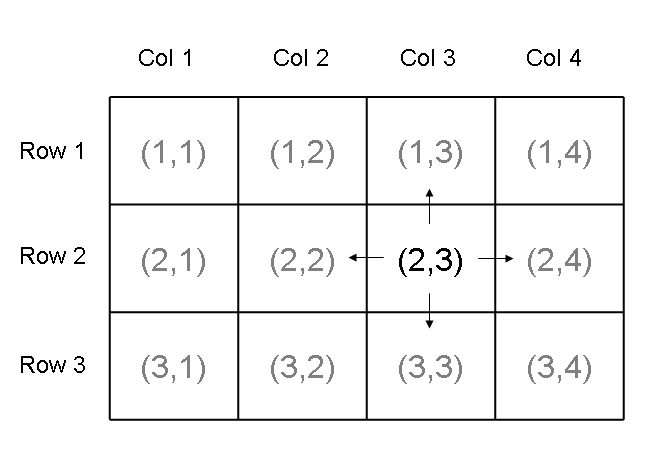
\includegraphics[width=0.66\textwidth]{Figures/SquareStructure}
  \caption{An illustration of the spatial structure}
  \label{fig:SquareSpatialStructure}
\end{figure}

Models are implemented as a grid of square cells making up a rectangular matrix. Distance between cells is determined as the euclidean\index{Inter-cell distance} distance between cell centres, modified by an arbitrary scalar. 

Hence, the definition of the spatial structure includes;
\begin{itemize}
\item The type of spatial grid and its dimensions, $n_{rows}$ and $n_{cols}$
\item The label of a numeric layer to be used as the base layer (defining the locations where the population can be present as well as the area of each cell)
\item The length (distance) of a side of the grid cell to be used as the scaler for distance calculations
\end{itemize}

For example, to specify a model with 3 rows and 4 columns (i.e., 12 spatial cells) with a base layer called \texttt{base} and 2 km sides of each cell, then the syntax for \texttt{@model} would include,
{\small{\begin{verbatim}
@model
nrows 3
ncols 4
layer base
cell_length 2
\end{verbatim}}}

See below for how to define a layer using \texttt{@layer}. 

\subsection{\I{Population structure}}

The population structure in \SPM\ is represented by a matrix containing an arbitrary number of user defined categories (rows), and an arbitrary age range (columns). Hence, each spatial cell has a population state described as $n_{categories} \times n_{ages}$ rectangular matrix with categories $k=1 \ldots n_{categories}$ and ages $l=age_{min} \ldots age_{max}$. 

The names and number of categories are user defined, but there must be at least one category defined for a model. The ages are defined as a sequence from $age_{min}$ to $age_{max}$, with the last age optionally a plus group. In order to calculate biomass, the age-size relationship for each category must also be defined.

Hence, the definition of the population structure includes;
\begin{itemize}
  \item The number and labels of the categories, $k_{categories}$
	\item The age\_size relationship for each category
  \item The minimum and maximum ages that define the ages of the model, $l_{ages}$
  \item If the last age is a plus group
\end{itemize}

For example, to specify a model with 2 categories (male and female) with ages 1-20 (with the last age a plus group) and an age-size relationship defined with the label \texttt{male-growth} and \texttt{female-growth}, then the \texttt{@model} example from above becomes,
{\small{\begin{verbatim}
@model
nrows 3
ncols 4
layer base
cell_length 2
categories male female
min_age 1
max_age 20
age_plus_group True
age_size male-growth female-growth
\end{verbatim}}}

See below for how to define age-size relationships using \texttt{@age\_size}. 

\subsection{\I{Layers}\label{sec:layers}}

Layers are a key underlying concept in \SPM. They comprise of a grid of known values, with a value for every spatial cell in the model. Layers are used by processes, observations, and outputs commands to supply spatially explicit covariates and any categorical groupings required. 

Layers are used by \SPM\ to evaluate locations where the population may be present (via the \emph{base layer}), to provide sets of known attributes or values of each spatial location (for some processes and for preference based movements), and to group or categorise cells for use by processes and observations. Layers consist of an $n_{rows} \times n_{cols}$ matrix and can be either \emph{numeric} or \emph{categorical}. 

Every model must define at least one layer, the base layer $L_B$. A layer is defined as a $n_{rows} \times n_{cols}$ matrix of values (albeit with the exception of layers that describe distance --- these are described in detail below), where the value in each cell represents a known quantity. For example layers may represent classifications, physical attributes, or some other known or assumed quantity. Typically they are provided by the user as a matrix of values, although some layers (e.g., abundance or distance layers) can be calculated by \SPM\ during a model run. 

Within \SPM, layers are used in the following contexts:
\begin{enumerate}
\item The base layer\index{Base layer}\index{Layers ! the base layer}: The base layer $L_B$ is a special layer (there must be exactly one base layer defined within the model) that defines the locations where the population can and cannot potentially be present (e.g., locations associated with the sea and not land in a marine model). Here, we define that a cell may potentially have part of the population present if every element $L_B(i,j) \ge 0$. Further, positive values of the base layer $L_B$ represent the \emph{area} represented by that spatial cell. Note, the values in the base layer must be numeric, but cannot be a meta-layer (\emph{see below}).
\item \I{Covariate layers}: A model may have many covariate layers, and these are used as covariates of some population or movement process (e.g., the sea floor depth may be a covariate of some movement process). The values in layers used as covariates can be either numeric or categorical.
\item \I{Classification layers}: A model may have many classification layers, and these are used as a classification or grouping variable for aggregating data over individual spatial cells $(i,j)$, e.g., statistical areas or management areas. Such layers are typically used to aggregate the population within cells into groups so-as to allow comparison with observations. The values in layers used as classification layers must be categorical.
\end{enumerate}

\SPM\ defines the following types of layer;

\begin{enumerate}
\item{\I{Numeric layers}\label{numeric-layer}}: A model may have many numeric layers, and these can be used as covariates of a population or movement process (e.g., depth may be a covariate of some movement process), and/or locations of event mortality. Numeric layers can contain only continuous (numeric) variables. Values for a numeric layer must be supplied for each cell by the user. Numeric layers can be rescaled to sum to some user-defined value, and unlike other layers, the values for each cell can be estimated. 

For example, to specify a numeric layer for a spatial model with $3 \times 4$ cells called, say \texttt{base}, with the top left and bottom right cells set to zero and all other cells set to one and not rescaled, use,
{\small{\begin{verbatim}
@layer base
type numeric
data 0 1 1 1
data 1 1 1 1
data 1 1 1 0
\end{verbatim}}}

\item {\I{Categorical layers}\label{categorical-layer}}: A model may have many categorical layers, and these can be used as a classification or grouping variable for aggregating data over individual cells, e.g., management areas; or as covariates of a population or movement process. Such layers are typically used to aggregate the population within cells into groups for comparing with observations, or to apply specific movement characteristics. The values in layers used as categorical layers can contain any characters (except white space), and are interpreted as categorical values. Values for a categorical layer must be supplied for each cell by the user.

For example, to specify a categorical layer for a spatial model with $3 \times 4$ cells called, say \texttt{zone}, with the top left cells allocated as zone \texttt{A}, the bottom right allocated as zone \texttt{C}, and the rest as zone \texttt{B}, then use,
{\small{\begin{verbatim}
@layer zone
type categorical
data A A B B
data A A C C
data B B C C
\end{verbatim}}}

\item {\I{Distance layers}}: A distance layer is one that defines the distance between cells. \SPM\ has four types of distance layer: (i) the Euclidean distance between cell centres (\texttt{distance})\index{Distance! Euclidean}\index{Euclidean distance}; (ii) the distance between two locations (defined by longitude and latitude) using the haversine formula (\texttt{haversine})\index{Distance! Haversine}\index{Haversine distance}; (iii) the shortest path between cells by traversing cell centres using \I{Dijkstra's algorithm} \citep{Dijkstra1959} and assumes that cells excluded by the base layer are not traversable (\texttt{dijkstra})\index{Distance! Dijkstra}\index{Dijkstra distance}; and (iv) the shortest path between cells using the Dijkstra's algorithm but with the  distances calculated using the haversine formula from latitudes and longitudes (\texttt{haversine\_dijkstra}).\index{Distance! Haversine Dijkstra}\index{Haversine Dijkstra distance}

The Euclidean distance method simply calculates the values of the distance layer as the Euclidean distance between the centres of every pair of cells, taking into account the length of the side of a cell. Here, the distance between cell $a$ and cell $b$ can be defined as,
\begin{equation}
  d(a,b) = \lambda \sqrt{(x_a - x_b)^2 + (y_a - y_b)^2}
\end{equation}
where $x$ and $y$ represent the x- and y-coordinates of $a$ and $b$ respectively, and $\lambda$ is an arbitrary scaler representing the length of one side of the square cell. Unlike other types of layers, distance layers are not a $n_{rows} \times n_{cols}$ grid of values, but rather a matrix of dimension $(n_{rows} \times n_{cols}) \times (n_{rows} \times n_{cols})$  where the distance between each cell and every other cell is evaluated. Note that the distance between any cell and itself is 0. 

For example, to specify a Euclidean distance layer, use,
{\small{\begin{verbatim}
@layer Distance
type distance
\end{verbatim}}}

The haversine method calculates the great-circle distance between two points on a sphere from the longitudes and latitudes of the cells, with the assumption that the Earth is a perfect sphere with radius exactly 6371 km. Two numeric layers are required, giving the longitude and latitude of each cell respectively. Latitude values must be between $-90^{\circ}$ (southern latitudes) and $90^{\circ}$ (northern latitudes). Longitude values must be between $0^{\circ}$ and $360^{\circ}$. Note that the distance between any cell and itself is 0.

For example, to specify a haversine distance layer for a $2\times3$ spatial model, assuming that latitudes and longitudes of each cell are given in the numeric layers labelled \texttt{cell\_latitudes} and \texttt{cell\_longitudes}, then use,
{\small{\begin{verbatim}
@layer cell_latitudes
type numeric
data -45 -45 -45
data -46 -46 -46

@layer cell_longitudes
type numeric
data 176 177 178
data 176 177 178

@layer Haversine_distance
type haversine
latitude cell_latitudes
longitude cell_longitudes
\end{verbatim}}}

The Dijkstra method calculates the distance between two points as the sum of the shortest path between cell centres that does not traverse through cells excluded by the base layer. Distances between adjacent cells are calculated using Euclidean distance as described above with $\lambda$ an arbitrary scaler representing the length of one side of each cell. Note that the distance between any cell and itself is 0.

For example, to specify a Dijkstra distance layer then use,

{\small{\begin{verbatim}
@layer Dijkstra_distance
type dijkstra
\end{verbatim}}}

The haversine-Dijkstra method calculates the distance between two points as the sum of the shortest path between cell centres that does not traverse through cells excluded by the base layer, where distances are calculated using the haversine formulae. Distances between adjacent cells are calculated using haversine distance as the great-circle distance between two points on a sphere from the longitudes and latitudes of the cell, with the assumption that the Earth is a perfect sphere with radius exactly 6371 km. Two numeric layers are required, giving the longitude and latitude of each cell respectively. Latitude values must be between $-90^{\circ}$ (southern latitudes) and $90^{\circ}$ (northern latitudes). Longitude values must be between $0^{\circ}$ and $360^{\circ}$. Note that the distance between any cell and itself is 0.

For example, to specify a haversine Dijkstra distance layer for a $2\times3$ spatial model, assuming that latitudes and longitudes of each cell are given in the numeric layers labelled \texttt{cell\_latitudes} and \texttt{cell\_longitudes}, then use,
{\small{\begin{verbatim}
@layer cell_latitudes
type numeric
data -45 -45 -45
data -46 -46 -46

@layer cell_longitudes
type numeric
data 176 177 178
data 176 177 178

@layer Haversine_Dijkstra
type haversine_dijkstra
latitude cell_latitudes
longitude cell_longitudes
\end{verbatim}}}

\item{\I{Abundance layers}}: The abundance layer is the sum of the number of individuals within cell $a$ in categories $k$ and with selectivity $S_l$ at age $l$. 
\begin{equation}
  N(a) = \sum\limits_{k} \sum\limits_l S_l \ \text{element}(i,j,k,l)
\end{equation}
\SPM\ calculates the values of the layer when running the model at the point in time where the value is required.

For example, to specify an abundance layer of all individuals who are categorised as \texttt{mature}, use,
{\small{\begin{verbatim}
@layer Abundance
type abundance
categories mature
selectivities One
\end{verbatim}}}

\item {\I{Biomass layers}}: The biomass layer is the sum of the biomass of individuals within cell $a$ in categories $k$, with selectivity $S_l$ at age $l$, and mean weight $w_{kl}$
\begin{equation}
  N(a) = \sum\limits_{k} \sum\limits_l w_{k,l} S_l \ \text{element}(i,j,k,l) 
\end{equation}
\SPM\ calculates the values of the layer when running the model at the point in time where the value is required.

For example, to specify a biomass layer of all individuals who are categorised as \texttt{mature}, use,
{\small{\begin{verbatim}
@layer Biomass
type biomass
categories mature
selectivities One
\end{verbatim}}}

\item {\I{Abundance-density layers}}: The abundance density layer is the density of the number of individuals within cell $a$ with area $A_a$ in categories $k$, with selectivity $S_l$ at age $l$,
\begin{equation}
  N(a) = \frac{1}{A_a} \sum\limits_{k} \sum\limits_l S_l \ \text{element}(i,j,k,l)
\end{equation}
\SPM\ calculates the values of the layer when running the model at the point in time where the value is required.

For example, to specify an abundance density layer of all individuals who are categorised as \texttt{mature}, use,
{\small{\begin{verbatim}
@layer AbundanceDensity
type abundance_density
categories mature
selectivities One
\end{verbatim}}}

\item {\I{Biomass-density layers}}: The biomass-density layer is the density of the biomass of individuals within cell $a$ with area $A_a$ in categories $k$, with selectivity $S_l$ at age $l$, and mean weight $w_{kl}$,
\begin{equation}
  N(a) = \frac{1}{A_a} \sum\limits_{k} \sum\limits_l w_{k,l} S_l \ \text{element}(i,j,k,l)
\end{equation}
\SPM\ calculates the values of the layer when running the model at the point in time where the value is required.

For example, to specify a biomass density layer of all individuals who are categorised as \texttt{mature}, use,
{\small{\begin{verbatim}
@layer BiomassDensity
type bioomass_density
categories mature
selectivities One
\end{verbatim}}}

\item {Derived quantity and derived quantity by cell layers}\label{derived quantity layer}\index{Derived quantity layers}\index{Derived quantity by cell layers}: \SPM\ can use values from a derived quantity or a derived quantity by cell as a layer. These are the values of a derived quantity, and require an offset (in years) to extract the desired value for each year. They will extract the derived quantity either for each cell (for derived quantities by cell) or as a total value applied to each cell (for ordinary derived quantities) as values for a layer.

For example, to specify a layer of the biomass of all individuals who are categorised as \texttt{mature} in time step \texttt{StepOne} from two years ago, first define a derived quantity,
{\small{\begin{verbatim}
@derived_quantity_by_cell Mature
type biomass
categories mature
selectivities One
time_step StepOne
\end{verbatim}}}

Then define the derived layer,
{\small{\begin{verbatim}
@layer MatureBiomass
type derived_quantity
derived_quantity Mature
year_offset 2
\end{verbatim}}}

\item {\I{Meta-layers}\label{meta-layers}}: \SPM\ defines a special type of layer known as a \emph{meta-layer}. Meta-layers allows individual layers to be indexed by year and applied as an annually varying layer within the model. For example, assume a model that uses Sea Surface Temperature (SST) as a layer, perhaps to drive some movement process. The SST values for each year of the model would be defined as individual layers, each with a unique label. A meta-layer could be defined that indexed the individual annual SST layers by year, and used as a covariate layer in the movement process. Meta-layers have a \emph{default} layer that is used for time periods that are not specifically defined. Meta layers can be used wherever ordinary layers are used (except that they cannot be used as the base layer), with \SPM\ extracting the appropriate layer value corresponding to the year or the initialisation phase.

\begin{enumerate}

\item {\I{Numeric meta-layers}\label{numeric meta-layer}}: Numeric meta-layers are a meta layer of numeric layers --- the individual ordinary layers that make up the meta-layer must all be of numeric type. For example, assuming that the layers \texttt{SST} and \texttt{SST1990}, \texttt{SST1995}, etc., are defined elsewhere, then to specify a numeric meta-layer with specific values for the years 1990-1995, and a default for all other years (including the initialisation phases), use, 

{\small{\begin{verbatim}
@layer AnnualNumericLayer
type numeric_meta
default_layer SST
years    1990    1991    1992    1993    1994    1995
layers SST1990 SST1991 SST1992 SST1993 SST1994 SST1995
\end{verbatim}}}

\item {\I{Categorical meta-layers}\label{categorical meta-layer}}: Categorical meta-layers are a meta layer of categorical layers --- the individual ordinary layers that make up the meta-layer must all be of categorical type. Categorical meta-layers are specified in the same way as numeric meta-layers. For example, assuming that the layers \texttt{zones} and \texttt{zone1990}, \texttt{zone1995}, etc., are defined elsewhere, then to specify a categorical meta-layer with specific values for the years 1990-1995, and a default for all other years (including the initialisation phases), use, 

{\small{\begin{verbatim}
@layer AnnualCategoricalLayer
type categorical_meta
default_layer zones
years     1990     1991     1992     1993     1994     1995
layers zone1990 zone1991 zone1992 zone1993 zone1994 zone1995
\end{verbatim}}}
\end{enumerate}
\end{enumerate}

\subsection{\I{Time sequences}}

The time sequence of the model is defined in two parts;
\begin{itemize}
  \item \I{Initialisation}
  \item \I{Run years}
  %\item \I{Projection year}s
\end{itemize}

\subsubsection{\I{Annual cycle}}

The annual cycle is implemented as a set of processes that occur, in a user-defined order, within each year. time-steps are used to break the annual cycle into separate components, and allow observations to be associated with different sets of processes. Any number of processes can occur within each time-step, in any order and can occur multiple times within each time-step. Note that time-steps during the initialisation phases can be different from that which is applied during the model years.

\subsubsection{\I{Initialisation}}

Model initialisation can occur in several phases\index{Initialisation!phases}, each which iterates through a number of years carrying out the population and/or spatial processes defined for that phase. At the end of the initialisation step, \SPM\ runs through the model years carrying out processes in the order defined in the annual cycle, and can evaluate expected values of observations in order to calculate likelihoods, %project forward to determine future states \NYI, 
or simulate observations from the current state.

\SPM\ initialises the initial equilibrium state as an iterative process: a general solution that initialises complex structured population and movement models can be difficult to implement using analytic techniques. However, initialising via iteration for a long-lived species with complex movements can take many iterations and hence be slow to run. In \SPM, we allow for user-defined multi-phased initialisation using iteration to allow the user to optimize models for speed. Each phase of the initialisation can involve any number of population and/or movement processes. Note that the length of the initialisation period may affect the model outputs, and that a period should be chosen to allow the population state to converge.

In addition, each initialisation process can optionally be stopped early if a user defined convergence criteria is met. For a set of user defined years in the initialisation phase, convergence is defined as met if the proportional absolute summed difference between the state in year $t-1$ and the state in year $t$ ($\widehat{\lambda}$) is less than $\lambda$ where, 
\begin{equation}
  \widehat{\lambda} = \frac{\sum\limits_{i} \sum\limits_{j} \sum\limits_{k} \sum\limits_l \left|\text{element}(i,j,k,l)_t - \text{element}(i,j,k,l)_{t-1} \right|}{\sum\limits_{i} \sum\limits_{j} \sum\limits_{k} \sum\limits_l \frac{}{}\text{element}(i,j,k,l)_t}
\end{equation}

Note that the check itself can be expensive time-wise, hence options exist for the user to request if or when this convergence check is carried out.

In each initialisation phase, the processes defined for that phase are carried out and used as the starting point for the following phase or, if it is the last phase, then the years that the model is run over. The first phase is always initialised with each element (i.e., each age and category within each spatial cell) set at zero. Note that this means that recruitment processes where the numbers of recruits is based on a stock recruitment or density dependant relationship will likely fail if used in the first phase of an initialisation. 

The multi-phase iteration\index{Multi-phase iteration} also allows the user to determine if the initialisation has converged in a particular model run. Here, add an additional initialisation phase for, say, $1$ year as the last initialisation phase (with the same processes applied). Then, using the initialisation reports (\commandlabsubarg{report}{type}{initialisation\_phase}), print a copy of the partition just before and just after that phase. If the initialisation has converged to an equilibrium state, then the partition at both these time intervals will be the same.

Hence, for initialisation you need to define;
\begin{itemize}
  \item The initialisation phases
  \item The number of years in each phase and the processes to apply in each
\end{itemize}

For example, to specify a model with a single phase of initialisation for 100 years (with a conve4rgence check at 80, 90, and 100 years) using time-steps \texttt{one} and \texttt{two}, then the \texttt{@model} example from above becomes,
{\small{\begin{verbatim}
@model
nrows 3
ncols 4
layer base
cell_length 2
categories male female
min_age 1
max_age 20
age_plus_group True
age_size male-growth female-growth
initialisation_phases phase1
\end{verbatim}}}

with the initialisation phases specified as,
{\small{\begin{verbatim}
@initialisation_phase phase1
years 100
time_steps one two
lambda 1e-10
lambda_years 80 90 100
\end{verbatim}}}

\subsubsection{\I{Model years}}

Following initialisation, the model then runs over a number of user-defined years. For this part of the model, the annual cycle can be broken into separate time-steps (see below). The model runs from the start of year \argument{initial} and runs to the end of year \argument{current}. %The projection part then extends the run time up to the end of year \argument{final}. 

For example, to specify a model for the years 1990--2010 , then the \texttt{@model} example from above becomes,
{\small{\begin{verbatim}
@model
nrows 3
ncols 4
layer base
cell_length 2
categories male female
min_age 1
max_age 20
age_plus_group True
age_size male-growth female-growth
initialisation_phases phase1
initial_year 1990
current_year 2010
\end{verbatim}}}

%\subsubsection{\I{Projections}\label{sec:projections}}
%
%\SPM\ can project, from a set of parameter estimates, the state of the model into the future \NYI. In a projection run, the model is initialised and run through the model years from \argument{initial} to the \argument{current}. Then, the model is run from \argument{current} to \argument{final}. 

\subsubsection{\I{Time-steps}}

The annual cycle is run during initialisation and over the model years. It is broken into time-steps. Within each time-step, processes are carried out in the order specified, and can be the same or different to processes in other time-steps or in the initialisation phases of the model. Further, observations (see later) can be associated with the state of the model at the end of a time-step --- i.e., time-steps are used to break the annual cycle into discrete 'chunks', and to allow the model to appropriately generate expected values for observations. 

For example, to specify a model with the time-steps \texttt{one} and \texttt{two}, and the processes \texttt{myRecruitment} and \texttt{myMaturation} in \texttt{one} and processes \texttt{myAgeing} and \texttt{myMortality} on \texttt{two}, then the \texttt{@model} example from above becomes,
{\small{\begin{verbatim}
@model
nrows 3
ncols 4
layer base
cell_length 2
categories male female
min_age 1
max_age 20
age_plus_group True
age_size male-growth female-growth
initialisation_phases phase1
initial_year 1990
current_year 2010
time\_steps one two
\end{verbatim}}}

with the time-step definitions 
{\small{\begin{verbatim}
@time_step one
processes myRecruitment myMaturation

@time_step two
processes myAgeing myMortality
\end{verbatim}}}

See later for how to define processes using \texttt{@process}. 

\subsection{\I{Processes}}

Processes produce changes in the model partition, by adding, removing or moving individuals between spatial cells (movement processes), and ages or categories (population processes). These include processes such as recruitment, mortality, ageing, and various forms of movement.

\SPM\ has two types of processes, \emph{population}\index{Population processes} and \emph{movement}\index{Movement processes} processes. Population processes are those processes which modify, move or otherwise change the numbers of individuals \emph{within} a spatial cell, i.e., they do not affect the spatial location of a cohort. Movement processes, on the other hand, move, shift or otherwise modify cohorts \emph{between} spatial cells, but do not affect the age or category of the numbers in each cohort. 

The population processes include recruitment\index{Recruitment}, ageing\index{Ageing},  mortality\index{Mortality} events (e.g., natural and exploitation) and category transition processes\index{Category transition} (i.e., processes that move individuals between categories, while preserving their age structure). See Section \ref{sec:population-section} for a complete list of available processes.

Each of these processes is carried out in the user-defined prescribed order when initialising the model, and then for a user-defined order in each year in the annual cycle\index{Annual cycle}.

\SPM\ implements three different types of movement processes\index{Movement};
\begin{enumerate}
	\item  A migration movement rate\index{Migration}\index{Movement ! Migration} of cohorts between any two locations, and is roughly analogous to movements between areas as implemented in other population models, such as CASAL \citep{1388}. 
	\item An adjacent cell movements\index{Adjacent cell movement}\index{Movement ! Adjacent cell movement}, parametrised by some function of an underlying layer --- equivalent to, for example, movement processes implemented in Fish Heaven \citep{1136,1135}. 
	\item Movement parametrised as a probability density function\index{Preference movement}\index{Movement ! Preference movement}. Here, the key underlying idea is that the spatial distribution of cohorts at any point in time and at any location can be represented as a density function based on attributes of that location, local abundance, and/or distance from their previous location \citep{1366,1367}. 
\end{enumerate}

An \SPM\ model can be parametrised by both population processes (for example, ageing, recruitment, and mortality), and movement processes. Population processes are those processes which modify, move or otherwise change the numbers of individuals within a spatial cell, i.e., they do not affect the spatial location of a cohort. Movement processes, on the other hand, move, shift or otherwise modify cohorts between spatial cells, but do not affect the age or category of the numbers in each cohort. 

\subsection{\I{Population processes}}

Population processes are those processes that change the population state of individuals, but retain their location. The population processes are described below.

\subsubsection{\I{Recruitment}}

Recruitment processes are defined as a process that introduces new individuals into the model. \SPM\ implements four types of recruitment process: constant recruitment\index{Recruitment ! Constant};  \I{Beverton-Holt recruitment}\index{Recruitment ! Beverton-Holt} \citep{1203}; \I{local Beverton-Holt recruitment}\index{Recruitment ! Local Beverton-Holt}; and recruitment proportional to an abundance or biomass \index{Proportional recruitment}\index{Recruitment ! proportional}.

In the recruitment processes, the number of individuals are added to a single age class within the partition, with the amount defined by the type of recruitment process and its function. If more than one category is defined, then the proportion of recruiting individuals to be added to each category is specified by the \argument{proportions} parameter. For example, if recruiting to categories labelled male and female, then you might set the proportions as $0.5$ and $0.5$ respectively to denote that half of the recruits recruit to the male category and the remaining half to the female category.

Recruitment occurs in those cells defined by a layer, or all cells if a layer has not been specified.

For the constant, Beverton-Holt, and proportional recruitment processes, the  number of individuals in cell cell$(i,j)$ following recruitment in year $y$ is,  
\begin{equation}
  \text{element}(i,j,k,l) \leftarrow \text{element}(i,j,k,l) + p_k(R_y / n) \frac{L_ij}{\sum_ij L_ij}
\end{equation}
where age is the age defined as the recruitment age, $p_k$ is the proportion to category $k$ defined to have recruitment, $n$ is the number of spatial locations where recruitment occurs, and the recruitment to each cell is scaled to be proportional to the value of the layer in that cell. See below for how $R_y$ is determined in each of these cases.

In the local Beverton-Holt recruitment process, individuals are recruited to an individual cell, based on the local abundance or biomass (i.e., the local SSB). For each cell where cell$(i,j)$ is a member of some layer $L_R$, the number of individuals in that cell following recruitment in each year $y$ is 
\begin{equation}
  \text{element}(i,j,k,l) \leftarrow \text{element}(i,j,k,l) + p_k R_y L_{ij}
\end{equation}
where age is the age defined as the recruitment age, $p_k$ is the proportion recruitment to category $k$ defined to have recruitment, and the recruitment to each cell is the product of the Beverton-Holt stock recruitment relationship ($R_y$). 

\subsubsection*{\I{Constant Recruitment}}

In the constant recruitment process the total number of recruits added each year is $R_y$, and is simply $R_0$, i.e.,
\begin{equation}
  R_y = R_0
\end{equation}

It is equivalent to a Beverton-Holt recruitment process where steepness is set equal to one ($h=1$).

For example, to specify a constant recruitment process, where individuals are added to the category `immature' at $age=1$, and the number to add is $R_0=5 \times 10^5$ in areas proportional to the value of the layer \texttt{recruitment}, then the syntax is,
{\small{\begin{verbatim}
@process Recruitment
type constant_recruitment
categories immature
proportions 1.0
R0 500000
age 1
layer recruitment
\end{verbatim}}}

\subsubsection*{\I{Beverton-Holt recruitment}}

In the Beverton-Holt recruitment process the total number of recruits added each year is $R_y$, and is the product of the average recruitment $R_0$, the annual year class strength multiplier, $YCS$, and the stock-recruit relationship i.e.,
\begin{equation}
  R_y = R_0 \times YCS_{y-offset} \times SR(SSB_{y-offset})
\end{equation}
  
where $offset$ is the number of years offset to link the year class with the year of spawning $y$, and $SR$ is the Beverton-Holt stock-recruit relationship parametrised by the steepness $h$,
\begin{equation}
SR(SSB_y) = \frac{SSB_y}{B_0} / \left( 1-\frac{5h-1}{4h} \left( 1-\frac{SSB_y}{B_0} \right) \right)
\end{equation}

Note that the Beverton-Holt recruitment process requires a value for $B_0$ and $SSB_y$ to resolve the stock-recruitment relationship. Here, a derived quantity (see Section \ref{sec:derived-quantities}) must be defined that provides the annual $SSB_y$ for the recruitment process. $B_0$ is then defined as the value of the $SSB$ at the end of one of the initialisation phases. During initialisation the YSC multipliers are assumed to be equal to one, and recruitment that happens in the initialisation phases that occur before and during the phase when $B_0$ is determined is assumed to have steepness $h=1$ (i.e. in those initialisation phases, recruitment is simply equal to $R_0$). Note it is an error if $B_0 <= 0$. 

Recruitment in the initialisation phases after the phase where $B_0$ follows the Beverton-Holt stock-recruit relationship defined above. Recruits are then distributed across cells in proportion to the values in a numeric layer. 

Year classes are standardised to be equal to one over the period $S$ defined by \texttt{standardise\_YCS\_years}, i.e., the year classes (YCS) for each year of the model are calculated as 
\begin{equation}
  YCS_i = \left\{
	   \begin{array}{ll}
     Y_i / mean_{y \in S}(Y_y) & : y \in S \\
	   Y_i & : y \notin S
  \end{array}
  \right.
\end{equation}

Note that the an effect of this parameterisation is that $R_0$ is then defined as the mean estimated recruitment over the years $S$, because the mean year class multiplier over these years will always be one.

For example, assume a Beverton-Holt recruitment process, where individuals are added to the category `immature' at $age=1$, the number to add is $R_0=5 \times 10^5$ in areas proportional to the value of the layer \texttt{MyRecruitment}. Then \texttt{SSB\_Biomass} is a derived quantity that specifies the total spawning stock biomass, with $B_0$ the value of the derived quantity at the end of the initialisation phase labelled \texttt{phase1}. The YCS are standardised to have mean one in the period 1994 to 2004, and recruits enter into the model two years following spawning. Then the command specification is,
{\small{\begin{verbatim}
@process Recruitment
type BH_recruitment
categories immature
proportions 1.0
R0 500000
steepness 0.75
age 1
layer MyRecruitment
B0 phase1
SSB SSB_Biomass
standardise_YCS_years 1994-2004
YCS_years 1994 1995 1996 1997 1998 1999 2000 2001 2002 2003 2004 2005 2006
YCS_values   1    1    1    1    1    1    1    1    1    1    1    1    1
SSB_offset 2
\end{verbatim}}}

Note that if not specified, $SSB\_offset$ is set at the value of $age$. This corresponds to cases where recruitment happens after spawning. $SSB\_offset$ can be user-defined to a different value if needed --- for example, if recruitment happens in a time-step before spawning, the offset will need to be specified as $age + 1$.

\subsubsection*{\I{Local Beverton-Holt recruitment}}

The local Beverton-Holt recruitment process assumes that, for recruitment, each cell acts like a local population and is independent of its neighbours. The value of the $SSB_y^i$ in each cell $i$ for each year $y$ is used to determine the amount of recruitment that enters that cell. If desired, these local recruits can subsequently be subjected to movement (see Section \ref{sec:movement-processes}).

If the recruitment to cell $i$ is $R_y^i$, then $R_y^i$ is the product of the average recruitment $R_0^i$ for that cell, the annual year class strength multiplier (assumed to be the same for all cells in each year), and the stock-recruit relationship, i.e., 
\begin{equation}
  R_y^i = R_0^i \times YCS_{y-offset} \times SR(SSB_{y-offset}^i)
\end{equation}
where $offset$ is the number of years offset to link the year class with the year of spawning, and $SR$ is the Beverton-Holt stock-recruit relationship parametrised by the steepness $h$ and initial biomass $B_0^i$
\begin{equation}
SR(SSB^i) = \frac{SSB^i}{B_0^i} / \left( 1-\frac{5h-1}{4h} \left( 1-\frac{SSB^i}{B_0^i} \right) \right)
\end{equation}

Note that the local Beverton-Holt recruitment process requires a value for $B_0^i$ and $SSB_y^i$ to resolve the stock-recruitment relationship. Here, a derived quantity by cell (see Section \ref{sec:derived-quantity-by-cell}) must be provided that defines $B_0$ and the annual $SSB_y$ for the recruitment process. As for the Beverton-Holt recruitment process above, $B_0$ is then defined as the value of the $SSB$ at the end of one of the initialisation phases. During initialisation the YSC multipliers are assumed to be equal to one, and recruitment that happens in the initialisation phases that occur before and during the phase when $B_0$ is determined is assumed to have steepness $h=1$ (i.e., in those initialisation phases, recruitment is simply equal to $R_0$). Recruitment in the initialisation phases after the phase where $B_0$ was determined follow the Beverton-Holt stock-recruit relationship defined above. If a layer is defined for recruitment, $R_0^i$ is defined for each cell as product of $R_0$ and the layer value in each cell. 

Year classes are standardised to be equal to one over the period $S$ defined by \texttt{standardise\_YCS\_years}, i.e., the year classes (YCS) for each year of the model are calculated as 
\begin{equation}
  YCS_i = \left\{
	   \begin{array}{ll}
     Y_i / mean_{y \in S}(Y_y) & : y \in S \\
	   Y_i & : y \notin S
  \end{array}
  \right.
\end{equation}

Note that the an effect of this parameterisation is that $R_0^i$ is then defined as the mean estimated recruitment over the years $S$, because the mean year class multiplier over these years will always be one.

For example, assume a local Beverton-Holt recruitment process, where individuals are added to the category `immature' at $age=1$, the number to recruit in each cell is $R_0=5 \times 10^5$ multiplied by the proportional value of the layer \texttt{MyRecruitment}. Then \texttt{SSB\_Biomass} is a derived quantity by cell that specifies the spawning stock biomass in each cell, with $B_0$ the value of the derived quantity at the end of the initialisation phase labelled \texttt{phase1}. The YCS are standardised to have mean one in the period 1994 to 2004, and recruits enter into the model two years following spawning. Then the command specification is,
{\small{\begin{verbatim}
@process Recruitment
type local_BH_recruitment
categories immature
proportions 1.0
R0 500000
steepness 0.75
age 1
layer MyRecruitment
B0 phase1
SSB SSB_Biomass
standardise_YCS_years 1994-2004
YCS_years 1994 1995 1996 1997 1998 1999 2000 2001 2002 2003 2004 2005 2006
YCS_values   1    1    1    1    1    1    1    1    1    1    1    1    1
SSB_offset 2
\end{verbatim}}}

Note that if not specified, $SSB\_offset$ is set at the value of $age$. This corresponds to cases where recruitment happens after spawning. $SSB\_offset$ can be user-defined to a different value if needed --- for example, if recruitment happens in a time-step before spawning, the offset will need to be specified as $age + 1$.

\subsubsection*{\I{Proportional recruitment}}

In the proportional recruitment process the total number of recruits added each year is $R_y$, and is the product of a multiplier ($\lambda$) and a measure of abundance or biomass, i.e.,
\begin{equation}
  R_y = \lambda \times SSB_{y-offset}
\end{equation}
 where $offset$ is the number of years offset to link the year class with the year of spawning $y$.

Note that the proportional recruitment process requires a value for $SSB_y$ in each year, with a default value that is applied in the initialisation phases where $SSB_y$ is not be available. Here, a derived quantity (see Section \ref{sec:derived-quantities}) must be defined that provides the annual $SSB_y$ for the recruitment process. $B_0$ is then defined as the value of the $SSB$ at the end of one of the initialisation phases. During initialisation the recruitment that happens in the initialisation phases that occur before and during the phase when $B_0$ is determined is assumed to be $R_0$. Recruitment in the initialisation phases after the phase where $B_0$ was determined follow the relationship defined above. Recruits are then distributed across cells in proportion to the values in a numeric layer. 

For example, assume a proportional recruitment process, where individuals are added to the category `immature' at $age=1$, the number to add is 0.5 the female breeding abundance, and placed into areas in proportion to the value of the layer \texttt{MyRecruitment}. The \texttt{female\_abundance} is a derived quantity by cell that specifies the total number of breeding females, with $B_0$ the value of the derived quantity at the end of the initialisation phase labelled \texttt{phase1}. Recruits enter into the model two years following spawning. Then the command specification is,
{\small{\begin{verbatim}
@process Recruitment
type proportional_recruitment
categories immature
proportions 1.0
lambda 0.5
R0 500000
age 1
layer MyRecruitment
B0 phase1
SSB female_abundance
SSB_offset 2
\end{verbatim}}}

Note that if not specified, $SSB\_offset$ is set at the value of $age$. This corresponds to cases where recruitment happens after spawning. $SSB\_offset$ can be user-defined to a different value if needed --- for example, if recruitment happens in a time-step before spawning, the offset will need to be specified as $age + 1$.

\subsubsection{\I{Ageing}\label{sec:ageing}}

The ageing process simply moves all individuals in the named categories to the next age class. The ageing process is defined as,
\begin{equation}
  \text{element}(i,j,k,l) \leftarrow \text{element}(i,j,k,l-1)
\end{equation}

except that in the case of the plus group (if defined), 
\begin{equation}
  \text{element}(i,j,k,age_{max}) \leftarrow \text{element}(i,j,k,age_{max}) + \text{element}(i,j,k,age_{max-1}).
\end{equation}

For example, to apply ageing to the categories \texttt{immature} and \texttt{mature}, then the syntax is,
{\small{\begin{verbatim}
@process Ageing
type ageing
categories immature mature
\end{verbatim}}}

Note that ageing is \emph{not} applied by \SPM\ by default. As with other processes, \SPM\ will not apply a process unless its defined and specified as a process within the annual cycle. Hence, it is possible to specify a model where a category is not aged. \SPM\ will not check or otherwise warn if there is a category defined where ageing is not applied.

\subsubsection{\I{Mortality}\label{sec:mortality}}

Six types of mortality processes are permissible in \SPM, constant rate, annually varying rate, event, biomass-event, a density-dependent relationship based on the Holling \citep{Holling1959} Type II or Type III function, and a density-dependent relationship based on prey-suitability process. These processes remove individuals from the partition, either as a rate (for constant or annually varying mortality processes), as a total number (abundance), or as a biomass of individuals. \SPM\ does not implement the Baranov catch equation or any other process where both natural and event mortality are applied simultaneously. To approximate concurrent natural and event mortality, the population processes must be defined to remove some natural mortality (e.g., as a constant or annually varying), then some event mortality (e.g., fishing) in sequence. It is up to the user to specify how this happens.

The constant rate, annually varying rate, event, biomass-event mortalities can depend on a layer. In these cases, the value of instantaneous mortality applied to the population state within each cell is the product of the layer value, a selectivity, and the mortality rate. If the layer is static, mortality is effectively constant each year but can be different in each cell; if the layer is a derived quantity and therefore calculated each year, mortality can change every year in every cell.

\subsubsection*{Constant mortality rate}

To specify an constant annual mortality rate \index{Constant mortality}($M=0.2$) for categories `male' and `female', then, 
{\small{\begin{verbatim}
@process NaturalMortality
type constant_mortality_rate
categories male female
selectivities One One
M 0.2 0.2
\end{verbatim}}}

Note that the mortality rate process requires a selectivity. To apply the same mortality rate over all age classes, use a selectivity defined as $S_i=1.0$ for all ages $i$, e.g.,
{\small{\begin{verbatim}
@selectivity One
type constant
c 1
\end{verbatim}}}

A constant rate could also be defined as a multiplier of a layer. For example, let the mortality rate applied to the population at cell $a$ in category $k$ and age $l$ be denoted $M(a,k,l)$, and given a value from a layer $L_a$  at $a$, a constant mortality rate $M$, and a selectivity-at-age $S_l$ at age $l$ for some user-defined categories $k$ then, 
\begin{equation}
  M(a,k,l) = ML_a S_l 
\end{equation}

And the resulting number of individuals remaining in cell $a$ in category $k$ at age $l$ from applying the constant mortality process is,
\begin{equation}
  n'(a,k,l) = n(a,k,l) \exp \left({-M(a,k,l)}\right)
\end{equation}

\subsubsection*{Constant exploitation rate}

To specify an constant annual exploitation rate \index{Constant exploitation}($P=0.2$) for categories `male' and `female', then, 
{\small{\begin{verbatim}
@process ExploitationMortality
type constant_exploitation_rate
categories male female
selectivities One One
P 0.2 0.2
\end{verbatim}}}

Note that the exploitation rate process requires a selectivity. To apply the same exploitation rate over all age classes, use a selectivity defined as $S_i=1.0$ for all ages $i$, e.g.,
{\small{\begin{verbatim}
@selectivity One
type constant
c 1
\end{verbatim}}}

A constant exploitation rate could also be defined as a multiplier of a layer. For example, let the exploitation rate applied to the population at cell $a$ in category $k$ and age $l$ be denoted $P(a,k,l)$, and given a value from a layer $L_a$  at $a$, a constant exploitation rate $P$, and a selectivity-at-age $S_l$ at age $l$ for some user-defined categories $k$ then, 
\begin{equation}
  P(a,k,l) = PL_a S_l 
\end{equation}

with $0<=P(a,l,k)<=1$.

And the resulting number of individuals remaining in cell $a$ in category $k$ at age $l$ from applying the constant mortality process is,
\begin{equation}
  n'(a,k,l) = n(a,k,l) P(a,k,l)
\end{equation}

\subsubsection*{Annual mortality rate}

Mortality for the annual rate\index{Annual mortality} is similar to the constant rate, except that rate applied each year is a separate parameter, and is applied equally to all of the specified categories. For example, if annual rates were applied to males and females between 1996 and 2000, five values of $M$ and the years that these apply to would need to be provided, e.g., 
{\small{\begin{verbatim}
@process AnnualMortality
type annual_mortality_rate
categories male female
selectivities One One
years 1996 1997 1998 1999 2000
M 0.20 0.15 0.22 0.25 0.21
\end{verbatim}}}

\subsubsection*{Event and biomass-event mortality}

The event mortality process\index{Event mortality} and biomass mortality processes act in a similar manner, except that they remove a specified abundance (number of individuals) or biomass respectively, rather than applying mortality as a rate. However, the maximum abundance or biomass to remove is constrained by a maximum exploitation rate.

The event mortality types must be defined using a layer. Here, the abundance or biomass to remove from a the population for each cell $a$ is the value of the layer at $a$ (denoted $F_a$) --- except where there are too few individuals for the event mortality to be taken (as defined by the maximum exploitation rate). In this scenario, \SPM\ removes as many individuals or as much biomass as it can while not exceeding the maximum exploitation rate. Event mortality processes require a penalty function to discourage parameter values that do not allow a the defined number of individuals to be removed. Here, the model penalises those parameter estimates that result in an insufficient number of individuals in defined categories (after applying selectivities). See Section \ref{sec:penalties} for more information on specifying penalties.

For example, the event mortality applied to user-defined categories $k$, with the numbers removed at age $l$ determined by a selectivity-at-age $S_l$ is applied as follows:

First, calculate the vulnerable abundance for each category $k$ in $1 \ldots K$ for ages $l = 1 \ldots L$ that are subject to event mortality,
\begin{equation}
  V(k,l) = S(l) N(k,l)
\end{equation}

And hence define the total vulnerable abundance $V_{total}$ as,
\begin{equation}
  V_{total}  = \sum\limits_K {\sum\limits_L {V(k,l)}} 
\end{equation}

Hence the exploitation rate\index{Maximum exploitation rate} to apply is 
\begin{equation}
U = \begin{cases}
  C/V_{total}, & \text{if $C/V_{total} \leq U_{max}$} \\
  U_{max}, & \text{otherwise}\\ 
  \end{cases} 
\end{equation}

And the number removed $R$ from each age $l$ in category $k$ is,
\begin{equation}
  R(k,l) = UV(k,l)
\end{equation}

For example, to specify fishing mortality based on spatially explicit catches (and given for each year as a layer, `Catch2000', `Catch2001', etc.) over categories `immature' and 'mature' with selectivity `FishingSel' and assuming a maximum possible exploitation rate of 0.7, then the syntax is,
{\small{\begin{verbatim}
@process Fishing
type event_mortality
categories immature mature
years 2000 2001 2002 2003
layers Catch2000 Catch2001 Catch2002 Catch2003
U_max 0.70
selectivities FishingSel FishingSel
penalty event_mortality_penalty
\end{verbatim}}}

\subsubsection*{Holling mortality rate}

The density-dependent Holling mortality process\index{Holling mortality} applies the Holling Type II and Type III functions \citep{Holling1959}, but is generalised using the Michaelis-Menten equation \citep{MentenMichaelis1913}. The function removes a number or biomass from a set of categories according to their total (selected) abundance (or biomass)and some 'predator' abundance (or biomass), but constrained by a maximum exploitation rate.

For example, the mortality applied to user-defined categories $k$, with the numbers removed at age $l$ determined by a selectivity-at-age $S(l)$ is applied as follows:

First, calculate the total predator abundance (or biomass) over all predator categories $k$ in $1 \ldots K$ and ages $l = 1 \ldots L$ that are applying the mortality,
\begin{equation}
  P(k,l) = S_{predator}(l) N_{predator}(k,l)
\end{equation}

And define the total predator abundance (or biomass) $P_{total}$ as,
\begin{equation}
  P_{total}  = \sum\limits_K {\sum\limits_L {P(k,l)}} 
\end{equation}

Then, calculate the total vulnerable abundance (or biomass) over all prey categories $k$ in $1 \ldots K$ and ages $l = 1 \ldots L$ that are subject to the mortality,
\begin{equation}
  V(k,l) = S_{prey}(l) N_{prey}(k,l)
\end{equation}

And hence define the total vulnerable abundance (or biomass) $V_{total}$ as,
\begin{equation}
  V_{total}  = \sum\limits_K {\sum\limits_L {V(k,l)}} 
\end{equation}

and then, the the number to remove is determined as,
\begin{equation}
R_{total} = P_{total} \frac{a  V_{total}^{x-1}}{b + V_{total}^{x-1}}
\end{equation}
where $x=2$ for Holling type II function,  $x=3$ for Holling type III function, or any value of $x \geq 1$ for the generalised Michaelis-Menten function, and $a > 0$ and $b > 0$ are the Holling function parameters.

Hence the exploitation rate\index{Maximum exploitation rate} to apply is 
\begin{equation}
U = \begin{cases}
  R_{total}/V_{total}, & \text{if $R_{total}/V_{total} \leq U_{max}$} \\
  U_{max}, & \text{otherwise}\\ 
  \end{cases} 
\end{equation}

And the number removed $R$ from each age $l$ in category $k$ is,
\begin{equation}
  R(k,l) = UV(k,l)
\end{equation}

The density-dependent Holling mortality process is applied either as a biomass or an abundance depending on the value of the \subcommand{is\_abundance} switch.

For example, a biomass Holling type II mortality process on \texttt{prey} by our predator \texttt{predator} would have syntax,

{\small{\begin{verbatim}
@process HollingMortality
type Holling_mortality_rate
is_abundance F
a 0.08
b 10000
x 2
categories prey
selectivities One
predator_categories predator
predator_selectivities One
u_max 0.8
\end{verbatim}}}

\subsubsection*{Prey-suitability mortality}

The density-dependent prey-suitability process\index{Density-dependent prey-suitability} applies predation mortality from a predator group to its prey groups simultaneously. It removes an abundance (or biomass) from each prey group according to the total (selected) abundance (or biomass) of each prey group, the total (selected) abundance (or biomass) of the other prey groups, some 'predator' abundance (or biomass), and the preference (electivity) of the predator to each prey group, but constrained by a maximum exploitation rate. The predator-prey suitability functions were based on the multispecies Virtual Population Analysis (MSVPA) functions described by \citep{JuradoMolina2005}.

For example, the mortality applied to the user-defined prey group $g$ of category $k$, with the numbers removed at age $l$ determined by a selectivity-at-age $S(l)$ is applied as follows:

First, calculate the total predator abundance (or biomass) over all predator categories $k$ in $1 \ldots K$ and ages $l = 1 \ldots L$ that are applying the mortality,
\begin{equation}
  P(k,l) = S_{predator}(l) N_{predator}(k,l)
\end{equation}

And define the total predator abundance (or biomass) $P_{total}$ as,
\begin{equation}
  P_{total}  = \sum\limits_K {\sum\limits_L {P(k,l)}} 
\end{equation}

Then, given the total vulnerable abundance (or biomass) of prey group $g$ over all categories $k$ in $1 \ldots K$ and ages $l = 1 \ldots L$ that are subject to the mortality,
\begin{equation}
  V(g,k,l) = S_{prey}(l) N_{prey}(k,l)
\end{equation}

And define the total vulnerable abundance (or biomass) of each prey group $V(g)_{total}$ as,
\begin{equation}
  V(g)_{total}  = \sum\limits_K {\sum\limits_L {V(g,k,l)}} 
\end{equation}

And the total availability $A(g)_{total}$ for each prey group as,
\begin{equation}
  A(g)_{total} = \frac{V(g)_{total}}{\sum\limits_G {V(i)_{total}}}
\end{equation}

The vulnerable abundance (or biomass) and availability every prey group $g$ in $1 \ldots G$ is calculated simultaneously. Then the abundance (or biomass) to remove from each prey group $g$ is a function of its electivity $E(g)$, the availability of all other prey groups $i$ in $1 \ldots G$, the electivity of the predator for each prey group $E(i)$, and the total consumption rate of the predator $CR$ and its abundance (or biomass) $P_{total}$,
\begin{equation}
  R(g)_{total}=P_{total} CR \frac{A(g)_{total} E(g)}{\sum\limits_G {A(i)_{total} E(i)}}
\end{equation}

Hence the exploitation rate\index{Maximum exploitation rate} to apply to each prey group $g$ is 
\begin{equation}
U(g) = \begin{cases}
  R(g)_{total}/V(g)_{total}, & \text{if $R(g)_{total}/V(g)_{total} \leq U_{max}$} \\
  U_{max}, & \text{otherwise}\\ 
  \end{cases} 
\end{equation}

And the number removed $R(g)$ in each prey group $g$ from each age $l$ in category $k$ is,
\begin{equation}
  R(g,k,l) = U(g)V(g,k,l)
\end{equation}

Note that prey suitability choice occurs only between prey groups specified by the process, and the total predator consumption rate represents the consumption of the predator on those prey groups alone. Also note that the electivities must sum to one. Further, the consumption rate can be modified by a layer, to be cell specific. 

The density-dependent prey-suitability process is applied as either a biomass or an abundance depending on the value of the \subcommand{is\_abundance} switch.

Individual categories can be aggregated into prey groups using the '+' symbol. To indicate that two (or more) categories are to be aggregated, separate them with a '+' symbol. For example, to specify two prey groups of two species made up of the males and females in each, then the subcommand would be,

{\small{\begin{verbatim}
prey_categories maleSpeciesA + femaleSpeciesA maleSpeciesB + femaleSpeciesB
\end{verbatim}}}

This would indicate that there are two prey groups, \texttt{maleSpeciesA + femaleSpeciesA} and \texttt{maleSpeciesB + femaleSpeciesB}, with each group having its own electivity. For example, a biomass prey-suitability mortality process with an overall consumption rate of $0.8$ of \texttt{species A} and \texttt{species B} (modelled as males and females) by our predator \texttt{predatorSpecies} with electivities between \texttt{species A} and \texttt{species B} of $0.18$ and $0.82$ would have syntax,

{\small{\begin{verbatim}
@process PreySuitabilityMortality
type prey-suitability_predation
is_abundance F
consumption_rate 0.8
categories maleSpeciesA + femaleSpeciesA maleSpeciesB + femaleSpeciesB
electivities 0.18 0.82
selectivities One One One One
predator_categories predatorSpecies
predator_selectivities One
u_max 0.8
\end{verbatim}}}

\subsubsection{\I{Category state}s}

Category state processes set the number of individuals at each age and category at a specified point in time during the model. \SPM\ implements only one type, the number in each age class and category in each cell (category state by age).

\subsubsection*{\I{Category state by age process}}

The category state by age process\index{Category state by age} sets the number $n$ in each age for a single category in each cell. This process may be used, for example, to initialise the partition at the start of a model for simulations or other scenario testing. The process for category $a$ and age $l$ in cell$(i,j)$ is,
\begin{equation}\begin{split}
  & \text{element}(i,j,a,l) \leftarrow N(i,j,a,l)
\end{split}\end{equation}

Note that this process will overwrite the information that may already exist within a spatial cell --- cells that are not defined will be left with their original values. Similarly, this process will overwrite the information that may already exist within the defined age classes in the specified category --- age classes that are not defined will be left with their original values. 

Only a single category can be defined --- use multiple processes to specify multiple categories. For example, to initialise the immature category in the partition, then you might define the category state processes \texttt{immature} as a process to run during an initialisation phase, with the process defined as,
{\small{\begin{verbatim}
@process initialise-immature
type category_state_by_age
category immature
layer Area
min_age 1
max_age 5
N A 2 5 15 8 12
N B 2 5 20 20 8
\end{verbatim}}}

where the layer specifies how the number of individuals are assigned to individual cells. In this example, assuming a $2 \times 2$ spatial model with the categorical layer (e.g., with label \texttt{Area}) defined as,
{\small{\begin{verbatim}
@layer Area
type categorical
data A A 
data B B
\end{verbatim}}}

then the state in the initialisation with label \texttt{phase1} would be set to,
{\small{\begin{verbatim}
cell  age=1 age=2 age=3 age=4 age=5 age=6
r1-c1     1   2.5   7.5     4     6     0
r1-c2     1   2.5   7.5     4     6     0
r2-c1     1   2.5    10    10     4     0
r2-c2     1   2.5    10    10     4     0 
\end{verbatim}}}

assuming that there were no age $6$ individuals previously in the partition. 

\subsubsection{\I{Category transition}s}

Category transition processes move individuals between categories. \SPM\ implements three types, the total number in each cell (category transition), a rate in each cell (category transition rate), and the number in each age class in each cell (category transition by age).

\subsubsection*{\I{Category transition process}}

The category transition process\index{Category transition} moves a number $n$ from some source to a sink category (or categories). This process may be used, for example, to implement a 'tagging' process for mark-recapture data. The transition process with selectivity $S$ for source category $a$ and sink category $b$ (in cell$(i,j)$ and age $l$) is,
\begin{equation}\begin{split}
  & \text{element}(i,j,a,l) \leftarrow \text{element}(i,j,a,l) - \frac{nS_l}{\sum\limits_l S_l} \times \text{element}(i,j,a,l) \\
  & \text{element}(i,j,b,l) \leftarrow \text{element}(i,j,b,l) + \frac{nS_l}{\sum\limits_l S_l} \times \text{element}(i,j,a,l)
\end{split}\end{equation}

The category transition process requires a penalty function to discourage parameter values that do not allow the specified number of individuals to be moved. Here, the model penalises those parameter estimates that result in an insufficient number of individuals in the source category (after applying the selectivity) available to be moved. See Section \ref{sec:penalties} for more information on specifying penalties.

If multiple categories of sources or sinks are defined, then they must be defined in `pairs'. The proportions of selected individuals in the source categories is used to define the proportions of individuals `moved' to the sink categories, as defined by the order that they are specified. For example, to `tag' a population of immature and mature individuals, then you might define a category transition process \texttt{tagging} with selectivities \texttt{tagging-Sel}, as,
{\small{\begin{verbatim}
@process tagging
type category_transition
from immature mature
selectivities tagging-Sel tagging-Sel
to immature-tag mature-tag
years 2001 2002 2003
layers TagRelease2001 TagRelease2002 TagRelease2003
penalty tag_release_penalty
\end{verbatim}}}

Note that this syntax can be used to combine individuals into categories, simply by repeating a category label when specifying the sink categories. Similarly, individuals within a category can be split into more than one category by repeating a category label when specifying the source categories.

\subsubsection*{\I{Category transition rate process}}

The category transition rate process\index{Category transition} moves a proportion $p$ from a source category to a and sink category (or categories). The category transition rate process with selectivity $S$ for source category $a$ and sink category $b$ (in cell$(i,j)$ and age $l$) is,
\begin{equation}\begin{split}
  & \text{element}(i,j,a,l) \leftarrow \text{element}(i,j,a,l) - pS_l \times \text{element}(i,j,a,l) \\
  & \text{element}(i,j,b,l) \leftarrow \text{element}(i,j,b,l) + pS_l \times \text{element}(i,j,a,l)
\end{split}\end{equation}

If multiple categories of sources or sinks are defined, then they must be defined in `pairs'. \SPM\ treats each pair of categories as an independent transition --- but note that these are applied in order that they are specified. For example, to `mature' males and females in a model with four categories \texttt{male-immature}, \texttt{female-immature}, \texttt{male-mature}, and \texttt{female-mature}, then you might define a category transition process \texttt{maturation} with selectivities \texttt{male-maturity} and \texttt{female-maturity}, as,
{\small{\begin{verbatim}
@process maturation
type category_transition_rate
from male-immature female-immature
to male-mature female-mature
proportions 1.0 1.0
selectivities male-maturity female-maturity
\end{verbatim}}}

Note that this syntax can be used to combine individuals into categories, simply by repeating a category label when specifying the sink categories. Similarly, individuals within a category can be split into more than one category by repeating a category label when specifying the source categories.

\subsubsection*{\I{Category transition by age process}}

The category transition by age process\index{Category transition} moves a number $n$ for each age class from some source to a sink category (or categories) in a given year in subsets of cells defined by a categorical layer. This process may be used, for example, to implement a 'tagging' process for mark-recapture data, were the number of individuals tagged at each age are known. If the process is to be applied over more than one year, multiple category transition processes by age will need to be defined --- one for each year. The transition process with selectivity $S$ for source category $a$ and sink category $b$ (in cell$(i,j)$ at age $l$) is,

\begin{equation}\begin{split}
  & \text{element}(i,j,a,l) \leftarrow \text{element}(i,j,a,l) - \frac{nS_l}{\sum\limits_l S_l} \times \text{element}(i,j,a,l) \\
  & \text{element}(i,j,b,l) \leftarrow \text{element}(i,j,b,l) + \frac{nS_l}{\sum\limits_l S_l} \times \text{element}(i,j,a,l)
\end{split}\end{equation}

Category transition by age processes require a penalty function to discourage parameter values that do not allow the specified number of individuals to be moved. Here, the model penalises those parameter estimates that result in an insufficient number of individuals in the source category (after applying the selectivity) available to be moved. See Section \ref{sec:penalties} for more information on specifying penalties.

If multiple categories of sources or sinks are defined, then they must be defined in `pairs'. The proportions of selected individuals in the source categories is used to define the proportions of individuals `moved' to the sink categories, as defined by the order that they are specified. For example, to `tag' a population of immature and mature individuals, then you might define a category transition process \texttt{tagging} with selectivities \texttt{tagging-Sel}, as,

For example, in a $2 \times 2$ spatial model a categorical layer (e.g., with label Area) may define that cells $(1,1)$ and $(1,2)$ have value $A$ and cells $(2,1)$ and $(2,2)$ have value $B$, i.e.,
{\small{\begin{verbatim}
@layer Area
type categorical
data A A 
data B B
\end{verbatim}}}

Then the category transition by age process that moves $40$ individuals in the subset of cells with label $A$ and $55$ individuals in the subset of cells with label $B$ may be defined as, 
{\small{\begin{verbatim}
@process tagging
type category_transition_by_age
from immature mature
to immature-tag mature-tag
layer Area
year 2001
min_age 1
max_age 5
N A 1 5 15 8 11
N B 2 5 20 20 8
penalty tag_release_penalty
\end{verbatim}}}

Note that this syntax can be used to combine individuals into categories, simply by repeating a category label when specifying the sink categories. Similarly, individuals within a category can be split into more than one category by repeating a category label when specifying the source categories.

\subsection{\I{Movement processes}\label{sec:movement-processes}}

Movement processes are those processes that move individuals between cells but retain their population state, and are defined such that,
\begin{equation}
\text{element}(i,j,k,l)\leftarrow \text{element}(i,j,k,l) + p \times \text{element}(i',j',k,l)
\end{equation}

i.e., each element in cell$(i,j)$ is updated as the sum of itself and some proportion $p$ of a neighbouring element in cell$(i',j')$. To conserve abundance we also update element$(i',j',k,l)$ as,
\begin{equation}
\text{element}(i',j',k,l)\leftarrow \text{element}(i',j',k,l) - p\times \text{element}(i',j',k,l)
\end{equation}

\SPM\ assumes that each movement process occurs simultaneously over all cells (synchronous updating), i.e., all cell updates from each individual movement process are first evaluated for all cells, and then applied to all cells affected. 

\SPM\ implements three types of movement\index{Movement};
\begin{enumerate}
	\item  A migration movement rate of cohorts between any two locations, and is roughly analogous to movements between areas as implemented in other population models, such as CASAL \citep{1388}.
	\item An adjacent cell movements, parametrised by some function of an underlying layer --- equivalent to, for example, movement processes implemented in Fish Heaven \citep{1136,1135}. 
	\item Movement parametrised as a probability density function. Here, the key underlying idea is that the spatial distribution of cohorts at any point in time and at any location can be represented as a density function based on attributes of that location, local abundance, and/or distance from their previous location \citep{1366,1367}. 
\end{enumerate}

\subsubsection{\I{Migration movement}}

The migration process moves individuals from one sets of locations (the source, or emigration layer) to another set of locations (the sink, or immigration layer). A migration can involve one or more categories. The emigration at age is defined as some constant proportion multiplied by a selectivity and the source layer applied as a proportion. The immigration at age is defined as the number emigrating at age distributed proportionally into the sink layer. Migrations are similar to the migration process used in some limited space models such as CASAL \citep{1388}.

For example, let the emigration applied to the population at cell $a$ in category $k$ and age $l$ be denoted $E(a,k,l)$, and given a value from an source layer $Le_a$  at $a$, a constant migration proportion $P$, and a selectivity-at-age $S_l$ at age $l$ for some user-defined categories $k$ then, 
\begin{equation}
  E(a,k,l) = \frac{P Le_a S_l }{\sum\limits_a Le_a}
\end{equation}

And let the immigration applied to the population at cell $a$ in category $k$ and age $l$ be denoted $I(a,k,l)$, and given a value from an sink layer $Li_a$  at $a$, for some user-defined categories $k$ then, 
\begin{equation}
  I(a,k,l) = \frac{E(a,k,l) Li_a }{\sum\limits_a Li_a} 
\end{equation}

For example, to migrate 50\% of males from the top left cell to the three cells in the bottom right of a $3\times3$ model, then first define the layers to define the movement source and sinks, 

{\small{\begin{verbatim}
@layer source
type numeric
data 1 0 0
data 0 0 0
data 0 0 0
\end{verbatim}}}

{\small{\begin{verbatim}
@layer sink
type numeric
data 0 0 0
data 0 0 1
data 0 1 1
\end{verbatim}}}

And then the migration is defined as,

{\small{\begin{verbatim}
@process MaleMigration
type migration
categories males
proportion 0.5
source_layer source
sink_layer sink
selectivities one
\end{verbatim}}}

\subsubsection{\I{Adjacent cell movement}}

The adjacent cell movement moves a proportion of individuals in each cell to its four neighbouring cells, and hence mimics a simple diffusion process. It can be applied to a limited range of spatial locations and/or as a gradient by using a layer. An adjacent cell movement can involve one or more categories and movement at age is defined as some constant proportion multiplied by a selectivity and the diffusion layer as a proportion over the four adjoining cells. If no layer is supplied, the process moves the population equally to the adjacent cells (i.e., a constant 0.25 proportion is assumed for each of the adjacent cells).

For example, let the movement from cell $a$ to neighbouring cell $b$ in category $k$ and age $l$ be denoted $V(a,b,k,l)$, and given a value from layer $L_b$  at $b$, values from layer $L_n$ at the four neighbouring cells to $a$ (including cell $b$), a constant migration proportion $P$, and a selectivity-at-age $S_l$ at age $l$ for some user-defined categories $k$ then, 
\begin{equation}
  V(a,b,k,l) = \frac{P L_b S_l }{\sum\limits_4 L_n}
\end{equation}

The movement value of all cells into all their neighbouring cells are calculated simultaneously from the population layer at the time of movement, and the balance of all movements is returned.

For example, to move 50\% of females to adjacent cells but favouring movement towards the bottom right cells, then first define a gradient layer, 

{\small{\begin{verbatim}
@layer diffusion_layer
type numeric
data 1 1 1
data 1 2 2
data 1 2 4
\end{verbatim}}}

And then the movement is defined as,

{\small{\begin{verbatim}
@process diffusion
type adjacent_cell
categories female
proportion 0.5
layer diffusion_layer
selectivities one
\end{verbatim}}}

\subsubsection{\I{Preference movement}}

Preference movements allows movement from any $cell(a) \rightarrow cell(b)$, for $\forall a,b \in L_B$ and is implemented as a function of the product of up to $n$ independent \emph{preference functions}. We define the probability of moving from any cell $a$ to any cell $b$, for all $a,b \in L_B$, as a function of the relative preference for that cell. Here, we use the term \emph{preference function}\index{Preference function} \citep{1366,1367} to describe the movement probability distributions. 

We assume that the population and spatial extent are defined, and that there is a preference function that is a function of some (typically estimable) parameters and a spatially explicit set of known attributes.The preference function movement process allows the number of parameters describing movement to to reduced, and results in a movement process that is some function of some underlying property of each location. For example, if we assume that movement between areas was a function of the Euclidean distance between areas, we could model movement between any two areas as a linear decay or exponential decay function \citep{1366}. Alternately, if distribution and density were correlated with bathymetric depth for a marine organism, we might model the movement and distribution as a function of depth. 

Note that two forms of the preference movement algorithm are implemented in \SPM. They implement the same algorithm, except that the \commandsubarg{process}{type}{preference\_threaded}\index{Threads!preference functions}\ implements movement as a multi-threaded CPU process\index{Multi-threaded CPU process} (allowing multiple between cell movements to be evaluated by the computer simultaneously) and \commandsubarg{process}{type}{preference} implements movement as a single-threaded CPU process\index{Single-threaded CPU process}. The simultaneous evaluation of movements between cells in the multi-threaded movement process can result in a significantly faster processing time for an individual model (though, due to the thread management overhead, only for large models). Note that a consequence of this is that the order of calculations for the multi-thread and single-thread processes \emph{may} differ in some cases, and that this may result in a slightly different outcome.

\subsubsection*{The total preference function\index{Total preference function}}

Movement in \SPM\ can be defined as a probability distribution based on an underlying preference function. Here, we define the preference for a cell $x$ as the preference function $f_x(\theta_x,P(x))$, where $\theta_x$ are the parameters for $f_x$. So, given a set of $n$ attributes for cell $x$, we can define a preference function for each, and hence we define the aggregated or total preference function for any cell $x$ as the weighted product of individual preference functions,
\begin{equation}
  P_x=f_1(\theta_1,P_1(x))^{\alpha_1} \times f_2(\theta_2,P_2(x))^{\alpha_2} \times f_3(\theta_3,P_3(x))^{\alpha_3} \times \cdots \times f_n(\theta_n,P_n(x))^{\alpha_n}
\end{equation}

where $\alpha_i$ is an arbitrary weighting factor for attribute $i$. In order to avoid over-parameterisation, it is recommended that at least one $\alpha_i$ be fixed to the value of one.

Then we define the probability of moving from cell $a$ to any cell $b$ (where $b$ is defined as the set of all possible cells, including $a$),
\begin{equation}
  p(a\rightarrow b) = \frac{P_a}{\sum\limits_{i \in \forall b} P_i}
\end{equation}

Note that there are three forms of preference function,
\begin{enumerate}
\item Those that are a function of some underlying attribute of a cell, as defined by some arbitrary layer $L$
\item Those that are a function of the abundance or biomass (perhaps with a selectivity and for a subset of all categories) of each cell
\item Those that are a function of the distance between the sink and the source cells. 
\end{enumerate} 

Preference functions of the first type are determined only by the parameters of the preference function and some underlying, fixed, attribute. Preference functions of the others are dynamic, i.e. they depend on the relative locations of the cells or on the density of a cell at a particular point in time.

\subsubsection*{Preference functions\index{Preference function}}

Preference functions in \SPM\ include constant, Normal, double-Normal, logistic, inverse-logistic, Exponential, threshold, categorical, and monotonic categorical. These are defined as,

\begin{enumerate}
\item The constant preference function\index{Constant preference function}\index{Preference function ! Constant} has dependent variable $x$ and has no parameters, and is defined as,
\begin{equation}
f(x)=x$, where $0 \leq x \leq 1
\end{equation}

\item The Normal preference function\index{Normal preference function}\index{Preference function ! Normal} has dependent variable $x$ and parameters $\theta = (\mu,\sigma)$, and is defined as, 
\begin{equation}\
f(x | \mu, \sigma) = 2^{-[(x- \mu)/\sigma ]^2} 
\end{equation}
 
\item The double-Normal preference function\index{Double-normal preference function}\index{Preference function ! Double-Normal} has dependent variable $x$ and parameters $\theta=(\mu,\sigma_L,\sigma_R)$, and is defined as,
\begin{equation}
  f(x | \mu, \sigma_L, \sigma_R) = \begin{cases}
    2^{-[(x- \mu)/\sigma_L ]^2}, & \text{if $x \leq \mu$} \\
    2^{-[(x- \mu)/\sigma_R ]^2}, & \text{if $x \ge \mu$}\\
  \end{cases}
\end{equation} 

\item The Logistic preference function \index{Logistic preference function}\index{Preference function ! Logistic} has dependent variable $x$ and parameters $\theta = (a_{50},a_{to95})$, and is defined as,
\begin{equation}
  f(x | a_{50}, a_{to95}) = 1 / [1+19^{(a_{50}-x)/a_{to95}}]
\end{equation}

\item The inverse-Logistic preference function\index{Inverse-Logistic preference function}\index{Preference function ! Inverse-Logistic} has dependent variable $x$ and parameters $\theta = (a_{50},a_{to95})$, and is defined as,
\begin{equation}
  f(x | a_{50}, a_{to95}) =1- 1 / [1+19^{(a_{50}-x)/a_{to95}}]
\end{equation}

\item The Exponential preference function\index{Exponential preference function}\index{Preference function ! Exponential} has dependent variable $x$ and parameter $\theta = (\lambda)$, and is defined as,
\begin{equation}
  f(x | \lambda) =\exp(-\lambda x), \text{where $x \geq 0$ and $0$ otherwise}
\end{equation}

\item The threshold preference function\index{Threshold preference function}\index{Preference function ! Threshold} has dependent variable $x$ and parameters $\theta = (N,\lambda)$, and is defined as,
\begin{equation}
  f(x | N, \lambda) = \begin{cases}
    1, & \text{if $0 \le x \leq N$} \\
    1/\left({\frac{x}{N}}^\lambda\right), & \text{if $x \ge N$}\\
    0, & \text{otherwise}
  \end{cases}
\end{equation}

\item The categorical preference function\index{Categorical preference function}\index{Preference function ! Categorical} has dependent variables $x_i$ and parameters $\theta = (\lambda_i)$, and is defined so that for each value $x_i$, there is a corresponding parameter $\lambda_i$. 

Note that for the categorical preference function, the preference function is potentially over-parameterised if $\alpha \ne 1$. Typically the values of $x$ are supplied via a categorical layer, with $x_i$ representing the unique values of the layer.

\item The monotonic categorical preference function\index{Monotonic categorical preference function}\index{Preference function ! Monotonic categorical} has dependent variables $x_i$ and parameters $\theta = (\hat{\lambda}_i)$. As for the categorical preference function, it is defined so that for each $x_i$, there is a corresponding parameter $\hat{\lambda}_i = \lambda_i$ for the first unique value of $x_i$ and  $\hat{\lambda}_i = \lambda_i+ \lambda_{i-1}$ otherwise, and that $\forall{i}, \lambda_i \ge=0 $.

Note that for the monotonic categorical preference function, the preference function is potentially over-parameterised if $\alpha \ne 1$. Typically the values of $x$ are supplied via a categorical layer, with $x_i$ representing the unique values of the layer.

\end{enumerate}

For example, to define a preference based movement that is the combination of a preferred depth (assumed to be given in the layer \texttt{Depth}) and distance (given in, say, the layer \texttt{Distance}, first define the individual preference functions,

{\small{\begin{verbatim}
@preference_function Depth
type double_normal
alpha 1
layer Depth
mu 600
sigma_l 120
sigma_r 150
\end{verbatim}}}

{\small{\begin{verbatim}
@preference_function Distance
type exponential
alpha 1
lambda 0.005
layer Distance
\end{verbatim}}}

And then the preference based movement process is simply,

{\small{\begin{verbatim}
@process Move
type preference
categories males+females
preference_functions Distance Depth
\end{verbatim}}}

\subsection{\I{Derived quantities}\label{sec:derived-quantities}}

Some processes require, as arguments, a population value derived from the population state. These are termed \emph{derived quantities}. Derived quantities are values, calculated by \SPM\ as the end of a specified time-step in every year, and hence they have a single value for each year of the model. Derived quantities can be calculated as either an abundance or as a biomass. Abundance derived quantities are simply the count or sum of cells within some categories (after applying a selectivity) within cells defined by a layer. Biomass derived quantities are similar, except they are a measure of biomass. Derived quantities are also calculated during the initialisation phases, and hence the time-step during each phase must also be specified. If the initialisation time-steps are not specified, \SPM\ will calculate the derived quantity during the initialisation phases in every year, at the end of the annual cycle.

Derived quantities are required by some processes, for example the Beverton-Holt recruitment process. The Beverton-Holt recruitment process requires an equilibrium biomass ($B_0$) and annual spawning stock biomass values ($SSB_y$) to resolve the stock-recruit relationship. Here, these would be defined as the abundance or biomass of a part of the population at some point in the annual cycle for selected ages and categories, and would be calculated as a derived quantity.

As an example, to define a biomass derived quantity (say spawning stock biomass, SSB) for a model, evaluated at the end of the first time-step (labelled step\_one) in the initialisation phases (and assuming two initialisation phases) and at the end of the first time-step otherwise, over areas defined by a layer as the spawning ground but counting all `mature' individuals, we would use the syntax,

{\small{\begin{verbatim}
@derived_quantity SSB
type biomass
time_step step_one
initialisation_time_steps step_one step_one
categories mature
selectivities One
layer spawning_ground
\end{verbatim}}}

\subsection{\I{Derived quantities by cell}\label{sec:derived-quantity-by-cell}}

Some processes require, as arguments, a population value derived from the population state, but available for each cell of the population. These are termed \emph{derived quantities by cell}. Derived quantities by cell are a matrix of values, calculated by \SPM\ as the end of a specified time-step in every year, and hence they have a single value for each cell in each year of the model. Derived quantities by cell can be calculated as either an abundance or as a biomass. Abundance derived quantities by cell are simply the count or sum within each cell for some categories (after applying a selectivity). Biomass quantities by cell layers are similar, except they are a measure of biomass. Derived quantities by cell are also calculated during the initialisation phases, and hence the time-step during each phase must also be specified. If the initialisation time-steps are not specified, \SPM\ will calculate the derived quantity by cell during the initialisation phases in every year, at the end of the annual cycle.

Derived quantities by cell are \emph{required} by some processes, for example the local Beverton-Holt recruitment process. The local Beverton-Holt recruitment process requires an equilibrium biomass ($B_0$) and annual spawning stock biomass values ($SSB_y$) in each cell to resolve the stock-recruit relationship for each cell. Here, these would be defined as the abundance or biomass of a part of the population at some point in the annual cycle for selected ages and categories, and would be calculated as a derived quantity by cell.

As an example, to define a biomass derived quantity by cell (say spawning stock biomass, SSB) for a model, evaluated at the end of the first time-step (labelled step\_one) in the initialisation phases (and assuming two initialisation phases) and at the end of the first time-step otherwise, but counting all `mature' individuals, we would use the syntax,

{\small{\begin{verbatim}
@derived_quantity_by_cell SSB
type biomass
time_step step_one
initialisation_time_steps step_one step_one
categories mature
selectivities One
\end{verbatim}}}
%
%Both derived quantity by cell and meta-layers are calculated based on user-defined formula, which can use a combination of existing layers and parameters, and user-defined parameters. Parameters defined in the formula need to be provided with initial values. These parameters can be estimated using the estimation section (see Section \ref{sec:estimation-section}) as any other parameter. The formula are given as strings and \SPM\ resolves the string, hence applies the calculation in each cell of the layers separately. The following math functions, including parentheses, are implemented,  
%
%{\small{\begin{verbatim}
%+ - * / exp log(e) sqrt ^2 pow(a,b) cos sin
%\end{verbatim}}}
%
%For example, density dependent mortality based on diet selectivity can be implemented by applying a derived quantity by cell to a constant relationship mortality rate (see Section \ref{sec:mortality}). If predator $A$ of a previously-defined biomass layer $L_A$ has two potential preys $B$ and $C$ with estimable selectivity parameters $E_B$ and $E_C$ respectively of initial values 0.9 and 0.1, and with previously-defined biomass layers $L_B$ and $L_C$ respectively, the mortality layer $Lm_B$ of prey $B$ due to predation by predator $A$ applied as a constant relationship mortality rate can be defined as,
%\begin{equation}
%Lm_B = L_A \frac{E_B L_B}{E_B L_B + E_C L_C}
%\end{equation}
%
%The total mortality of prey $B$ can be defined as due to predation by predator $A$ only using a constant relationship mortality rate only, or as due to a combination of the mortality due to predation by predator $A$ and other mortalities (constant or layer-based) by defining other mortality events applicable to prey $B$ (see Section \ref{sec:mortality} for further details). The three biomass layers $L_A$, $L_B$, and $L_C$ need to be defined in the model as (derived) biomass layers of species $A$, $B$, and $C$ respectively at a specific time-step. These biomass layers as well as the mortality layer are updated each year by the model at the required time-step. The selectivity parameters can be fixed or estimated by the model with the given initial values.
%\TODOend

\subsection{\I{Size-age relationship}\label{sec:size-at-age}}

The age-size relationship defines the size at age (and the weight at size, see Section \ref{sec:mean-weight}) of individuals at age/category within the model. There are three size-age relationships available in \SPM. The first is the naive no relationship (where each individual has size 1 irrespective of age). The second  and third are the von-Bertalanffy and Schnute relationships respectively. The size-at-age relationship is used to determine the size frequency, given age, and then with the size-weight relationship, a weight-at-age of individuals within an age/category. 

The three age-size relationships are,

\begin{description}
\item {None:} where the size of each individual is exactly 1 for all ages, in which case the \texttt{none} size-weight relationship must also be used.
\item{von Bertalanffy:}\index{von Bertalanffy growth curve} where size at age is defined as,
\begin{equation} 
\bar{s}(age)= L_\infty \left( 1 - \exp \left( -k \left(age-t_0 \right) \right) \right)
\end{equation}

\item{Schnute:}\index{Schnute growth curve} where size at age is defined as,
\begin{equation}
\bar{s}(age)=\displaystyle\begin{cases}
  \left[ y_1^b + (y_2^b - y_1^b) \dfrac{1-\exp \left(-a(age - \tau_1) \right)}{1-\exp \left(-a(\tau_2 - \tau_1) \right)} \right]^{1/b}, & \text{if $a\ne0$ and $b\ne0$} \\
  \AddVspace
  y_1 \exp \left[ \ln \left( y_2 / y_1 \right) \dfrac{1-\exp \left(-a(age - \tau_1) \right)}{1-\exp \left(-a(\tau_2 - \tau_1) \right)} \right], & \text{if $a\ne0$ and $b=0$} \\
  \AddVspace
  \left[ y_1^b + \left( y_2^b - y_1^b \right) \dfrac{age-\tau_1}{\tau_2 - \tau_1} \right]^{1/b}, & \text{if $a=0$ and $b\ne0$} \\
  \AddVspace
  y_1 \exp \left[ \ln \left( y_2/y_1 \right) \dfrac{age-\tau_1}{\tau_2 - \tau_1} \right] , & \text{if $a=0$ and $b=0$} \\
  \end{cases}
\end{equation}
\end{description}

The von Bertalanffy curve is parameterised by $L_\infty$, $k$, and $t_0$; the Schnute curve \citep{836} by $y_1$ and $y_2$, which are the mean sizes at reference ages $\tau_1$ and $\tau_2$, and $a$ and $b$ (when $b=1$, this reduces to the von Bertalanffy with $k=a$). 

When defining size-at-age in \SPM, you must also define a size-weight relationship (see Section \ref{sec:mean-weight} below).

For example to define the age-at-size with label \texttt{VB} as a von-Bertalanffy relationship with $L_\infty=100$, $k=0.3$, and $t_0=-0.1$, and a size-weight relationship (see below) given by \texttt{SizeWeight},

{\small{\begin{verbatim}
@age_size VB
type von_bertalanffy
linf 100
k 0.3
t0 -0.1
size_weight SizeWeight
\end{verbatim}}}

\subsection{\I{Size-weight relationship}\label{sec:mean-weight}}

There are two size-weight relationship,s available in \SPM. The first is the naive no relationship. Here, the weight of an individual, regardless of size, is always 1. The second is the basic relationship. 

The two size-weight relationships are,

\begin{itemize}
  \item{None:} The size-weight relationship where  
  \begin{equation}
    \text{mean weight}=1
  \end{equation}
  \item{Basic:}\index{Basic size-weight relationship} The size-weight relationship where the mean weight $w$ of an individual of size $l$ is
  \begin{equation}
    w=a l^b
  \end{equation}
	Note that if a distribution of size-at-age is specified, then the mean weight is calculated over the distribution of sizes, and is
  \begin{equation}
	  w=(al^b)(1+cv^2)^{\frac{b(b-1)}{2}}
  \end{equation}
	where the $cv$ is the c.v. of sizes-at-age. This adjustment is exact for lognormal distributions, and a close approximation for normal distributions if the c.v. is not large \citep{1388}.
\end{itemize}

Be careful about the scale of $a$ --- this can easily be specified incorrectly. If the catch is in tonnes and the growth curve in centimetres, then $a$ should be on the right scale to convert a length in centimetres to a weight in tonnes. Note that there are reports available that can be used to help check that the units specified are plausible (see Section \ref{sec:report-section}).

For example to define the size-weight with label \texttt{SizeWeight} as the basic relationship with $a=1.4e-8$ and $b=3$,

{\small{\begin{verbatim}
@size_weight SizeWeight
type basic
a 1.4e-008
b 3
\end{verbatim}}}

\subsection{\I{Selectivities}\label{sec:selectivities}}

A selectivity is a function with a different value for each age class (i.e., for each column of the partition). Selectivities are used throughout \SPM\ to interpret observations (Section \ref{sec:estimation-section}) or to modify the effects of processes on each age class (Section \ref{sec:population-section}). \SPM\ implements a number of different parametric forms, including logistic, knife edge, and double normal selectivities.

A selectivity is always defined to apply just to one category of the population (i.e, row of the partition). To apply the same selectivity to more than one category, then just repeat the selectivity for each category that it is applied to.

Note that selectivities are indexed by age, with indices from \argument{min\_age} to \argument{max\_age}. For example, you might have an age-based selectivity that was logistic with $50\%$ selected at age $5$ and $95\%$ selected at age $7$. This would be defined by the \subcommand{type}=\argument{logistic} with parameters $a_{50}=5$ and $a_{to95}=(7-5)=2$. Then the value of the selectivity at age $x=7$ is $0.95$ and the selectivity at $x=3$ is $0.05$.

Note that the function values for some choices of parameters for some selectivities can result in an computer numeric overflow error (i.e., the number calculated from parameter values is either too large or too small to be represented in computer memory). \SPM\ implements range checks on some parameters to test for a possible numeric overflow error before attempting to calculate function values. For example, the logistic selectivity is implemented such that if $(a50-x)/ato_95 > 5$ then the value of the selectivity at $x=0$, i.e., for $a50=5$, $ato_95=0.1$, then the value of the selectivity at $x=1$, without range checking would be $7.1 \times 10^{-52}$. With range checking, that value is $0$ (as $(a50 x)/ato_95=40 > 5$).

The available selectivities are;

\begin{itemize}
  \item Constant
  \item Knife-edge
  \item All values
  \item All values bounded
  \item Increasing
  \item Logistic
	\item Inverse logistic
  \item Logistic producing
  \item Double normal
  \item Double exponential
	\item Cubic spline
\end{itemize}

The available selectivities are described below.

\subsubsection[Constant]{\argument{constant}}\index{Selectivities!Constant}

\begin{equation}
f(x)=C
\end{equation}

The constant selectivity has the estimable parameter C. 

For example, to define a constant selectivity with $c=1$, use,

{\small{\begin{verbatim}
@selectivity Sel
type constant
c 1
\end{verbatim}}}

\subsubsection[Knife-edge]{\argument{knife\_edge}}\index{Selectivities!Knife-edge}

\begin{equation}
f(x)= \begin{cases}
  0, & \text{if $x < E$} \\
  \alpha, & \text{if $x \ge E$}\\ 
  \end{cases} 
\end{equation}

The knife-edge selectivity has the estimable parameter $E$and a scaling parameter $\alpha$, where the default value of $\alpha = 1$

For example, to define a knife-edge selectivity with $=12$, use,

{\small{\begin{verbatim}
@selectivity Sel
type knife_edge
e 12
\end{verbatim}}}

\subsubsection[All-values]{\argument{all\_values}}\index{Selectivities!All-values}

\begin{equation}
f(x)=V_x
\end{equation}

The all-values selectivity has estimable parameters $V_{low}$, $V_{low+1}$ \ldots $V_{high}$. Here, you need to provide the selectivity value for each age class.

For example, to define an all-values selectivity for a model with ages $1 \ldots 6$, and the selectivity at age linearly increasing from $0$ to $1$ over those ages, use

{\small{\begin{verbatim}
@selectivity Sel
type all_values
v  0.0 0.2 0.4 0.6 0.8 1.0
\end{verbatim}}}

\subsubsection[All-values-bounded]{\argument{all\_values\_bounded}}\index{Selectivities!All-values-bounded}

\begin{equation}
f(x)=\begin{cases}
		 0, & \text{if $x < L$} \\
		 V_x, & \text{if $L \le x \le H$} \\
		 V_H, & \text{if $x > H$}
  \end{cases}
\end{equation}

The all-values-bounded selectivity has non-estimable parameters L and H. The estimable parameters are $V_L$, $V_{L+1}$ \ldots $V_H$. Here, you need to provide an selectivity value for each age class from $L \ldots H$.

For example, to define an all-values-bounded selectivity for a model with ages $1$ to $6$, and the selectivity at age linearly increasing from $0$ to $1$ over ages $1 \ldots 4$ and constant thereafter, use

{\small{\begin{verbatim}
@selectivity Sel
type all_values_bounded
l 1 
h 4 
v 0.0 0.33 0.66 1.0
\end{verbatim}}}

\subsubsection[Increasing]{\argument{increasing}}\index{Selectivities!Increasing}

\begin{equation} 
f(x)=\begin{cases}
	  0, & \text{if $x < L$} \\
	  f(x-1)+ \pi_x(\alpha-f(x-1)), & \text{if $L \le x \le H$} \\
	  f(\alpha), & \text{if $x \ge H$} \\  
  \end{cases}
\end{equation}

The increasing ogive has non-estimable parameters $L$ and $H$. The estimable parameters are $\pi_L$, $\pi_{L+1}$ \ldots $\pi_H$ (but if these are estimated, they should always be constrained to be between 0 and 1). $\alpha$ is a scaling parameter, with default value of $\alpha = 1$. Note that the increasing ogive is similar to the all-values-bounded ogive, but is constrained to be non-decreasing.

For example, to define an increasing selectivity for a model with ages $1$ to $6$, and the selectivity at age increasing by 0.1 from $0.5$ over ages $1 \ldots 4$ and constant thereafter, use

{\small{\begin{verbatim}
@selectivity Sel
type increasing
l 1 
h 4 
v 0.5 0.1 0.1 1.0
\end{verbatim}}}

\subsubsection[Logistic]{\argument{logistic}}\index{Selectivities!Logistic}

\begin{equation}
  f(x) = \alpha / [1+19^{(a_{50}-x)/a_{to95}}]
\end{equation}
 
The logistic selectivity has estimable parameters $a_{50}$ and $a_{to95}$. $\alpha$ is a scaling parameter, with default value of $\alpha = 1$. The logistic selectivity takes values $0.5 \alpha$ at $x=a_{50}$ and $0.95 \alpha$ at $x=a_{50}+a_{to95}$. 

For example, to define a logistic selectivity for a model with ages $1$ to $6$ with $a_{50}=3$ and $a_{to95}=1$, with a maximum selectivity of $1.0$, use

{\small{\begin{verbatim}
@selectivity Sel
type logistic
alpha 1
a50 4
ato95 1
\end{verbatim}}}

\subsubsection[Inverse logistic]{\argument{inverse\_logistic}}\I{Selectivities!Inverse-logistic}

\begin{equation}
  f(x) = \alpha - \alpha / [1+19^{(a_{50}-x)/a_{to95}}]
\end{equation}
 
The inverse-logistic selectivity has estimable parameters $a_{50}$ and $a_{to95}$. $\alpha$ is a scaling parameter, with default value of $\alpha = 1$. The logistic selectivity takes values $0.5 \alpha$ at $x=a_{50}$ and $0.95 \alpha$ at $x=a_{50}-a_{to95}$. 

For example, to define an inverse-logistic selectivity for a model with ages $1$ to $6$ with $a_{50}=3$ and $a_{to95}=1$, with a maximum selectivity of $1.0$, use

{\small{\begin{verbatim}
@selectivity Sel
type inverse_logistic
alpha 1
a50 4
ato95 1
\end{verbatim}}}

\subsubsection[Logistic producing]{\argument{logistic\_producing}}\index{Selectivities!Logistic-producing}

\begin{equation} 
f(x)=\begin{cases}
	  0, & \text{if $x < L$} \\
	  \lambda(L), & \text{if $x=L$} \\
	  \left( \lambda(x)-\lambda(x-1) \right) / \left( 1-\lambda(x-1) \right), & \text{if $L < x < H$} \\
	  1, & \text{if $x \ge H$} \\  
  \end{cases}
\end{equation}

The logistic-producing selectivity has the non-estimable parameters $L$ and $H$, and has estimable parameters $a_{50}$ and $a_{to95}$. $\alpha$ is a scaling parameter, with default value of $\alpha = 1$. For category transitions, $f(x)$ represents the proportion moving, not the proportion that have moved. This selectivity was designed for use in an age-based model to model maturity. In such a model, a logistic-producing maturation selectivity will (in the absence of other influences) make the proportions mature follow a logistic curve with parameters $a_{50}$, $a_{to95}$.

For example, to define an logistic-producing selectivity for a model with ages $1$ to $6$ with $a_{50}=3$ and $a_{to95}=1$, with a maximum selectivity of $1.0$, use

{\small{\begin{verbatim}
@selectivity Sel
type logistic_producing
alpha 1
l 1 
h 6
a50 4
ato95 1
\end{verbatim}}}

\subsubsection[Double-normal]{\argument{double\_normal}}\index{Selectivities!Double-normal}

\begin{equation}
  f(x) = \begin{cases}
    \alpha 2^{-[(x- \mu)/\sigma_L ]^2}, & \text{if $x \leq \mu$} \\
    \alpha 2^{-[(x- \mu)/\sigma_R ]^2}, & \text{if $x \ge \mu$}\\
  \end{cases}
\end{equation} 

The double-normal selectivity has estimable parameters $a_1$, $s_L$, and $s_R$. $\alpha$ is a scaling parameter, with default value of $\alpha = 1$. It has values $\alpha$ at $x=a_1$, and $0.5 \alpha$ at $x=a_1-s_L$ and $x=a_1+s_R$. 

For example, to define an double-normal selectivity for a model with ages $1$ to $6$ with $\mu=3$, $\sigma_L=1$, and $\sigma_R=1$, with a maximum selectivity of $1.0$, use

{\small{\begin{verbatim}
@selectivity Sel
type double_normal
alpha 1
mu 3
sigma_l 1
sigma_r 1
\end{verbatim}}}

\subsubsection[Double-exponential]{\argument{double\_exponential}}\index{Selectivities!Double-exponential}

\begin{equation} 
f(x)=\begin{cases}
	  \alpha y_0(y_1 / y_0)^{(x-x_0)/(x_1-x_0)}, & \text{if $x \le x_0$} \\
	  \alpha y_0(y_2 / y_0)^{(x-x_0)/(x_2-x_0)}, & \text{if $x > x_0$} \\
  \end{cases}
\end{equation}

The double-exponential selectivity has non-estimable parameters $x_1$ and $x_2$, and estimable parameters $x_0$, $y_0$, $y_1$, and $y_2$.  $\alpha$ is a scaling parameter, with default value of $\alpha = 1$. It can be `U-shaped'. Bounds for $x_0$ must be such that $x_1 < x_0 < x_2$. With $\alpha=1$, the selectivity passes through the points $(x_1, y_1)$, $(x_0, y_0)$, and $(x_2, y_2)$. If both $y_1$ and $y_2$ are greater than $y_0$ the selectivity is `U-shaped' with minimum at $(x_0, y_0)$.

For example, to define an double-exponential selectivity for a model with ages $1$ to $6$ that passes through the points $(1,1)$, $(3,0.1)$, and $(6,1)$, use 

{\small{\begin{verbatim}
@selectivity Sel
type double_exponential
alpha 1
x0 3
y0 0.1
x1 1
y1 1
x2 6
y2 1
\end{verbatim}}}

\subsubsection[Spline]{\argument{spline}}\index{Selectivities!Spline}

The spline selectivity implements a cubic spline that has non-estimable knots, and an estimable value for each knot. The cubic spline is either (i) a natural splines where the where the second derivatives are set to 0 at the boundaries, i.e., the values at the boundaries are horizontal, (ii) a spline with a fixed first derivative at the boundaries (linear, but not necessarily horizontal) and (iii) spline which turns into a parabola at the boundaries.

For example, to define a spline selectivity for a model with ages $1$ to $6$ with $3$ knots defined for the ages $1$, $3$, and $6$, and where the shape of the selectivity is horizontal at the ends, use

{\small{\begin{verbatim}
@selectivity Sel
type spline
alpha 1
knots 1 3 6
values 0.1 0.5 1.0
method natural
\end{verbatim}}}


\clearemptydoublepage{}
\section{\I{The estimation section}\label{sec:estimation-section}}

\subsection{Role of the estimation section\label{sec:role-of-the-estimation-section}}

The role of the estimation section is to define the tasks carried out by \SPM: 

\begin{enumerate}
  \item Define the objective function (see Section \ref{sec:objective-function})
  \item Define the parameters to be estimated (see Section \ref{sec:estimate-free-parameters})
  \item Calculate a point estimate, i.e., the maximum posterior density estimate (MPD) (see Section \ref{sec:estimate-MPD})\index{MPD}.
  \item Calculate a posterior profile selected parameters, i.e., find, for each of a series of values of a parameter, allowing the other estimated parameters to vary, the minimum value of the objective function (see Section \ref{sec:estimate-profiles}\index{Profiles}).
  \item Generate an MCMC sample from the posterior distribution (see Section \ref{sec:estimate-MCMC}\index{MCMC}).
  \item Calculate the approximate covariance matrix of the parameters as the inverse of the minimizer\textquoteright{}s approximation to the Hessian, and the corresponding correlation matrix (see Section \ref{sec:estimate-MPD}\index{Covariance matrix}).
\end{enumerate}

The estimation section defines 
The objective function is based on a goodness-of-fit measure of the model to observations, priors and penalties. The observation section describes the objective function, observations, priors and penalties. 

\subsection{\I{The objective function}\label{sec:objective-function}}

In Bayesian estimation, the objective function is a negative log-posterior,

\begin{equation}
Objective(p)= - \sum\limits_i {\log \left[ {L\left( {{\bf{p}}|O_i } \right)} \right]}  - \log \left[ {\pi \left( {\bf{p}} \right)} \right]
\end{equation}

where $\pi$ is the joint prior density of the parameters $p$.

The contribution to the objective function from the likelihoods are defined in Section \ref{sec:likelihoods}. In addition to likelihoods, priors (see Section \ref{sec:priors}) and penalties (see Section \ref{sec:penalties}) are components of the objective function. 

You will usually want to use penalties to ensure that the exploitation rate constraints on your fisheries are not breached (otherwise there is nothing to prevent the model from having abundances so low that the recorded catches could not have been taken), penalties on category transitions (to ensure there are enough individuals to move), and possibly penalties to encourage estimated values to be similar, smoothed, etc.

\subsection{\I{Specifying the parameters to be estimated}\label{sec:estimate-free-parameters}}

You need to tell SPM which of the estimable parameters are to be estimated by using \command{estimate} commands (see Section \ref{sec:estimation-syntax}). An \command{estimate} command-block looks like\index{Estimating parameters},

\begin{verbatim}
  @estimate process[MyRecruitment].r0
  lower_bound 1000
  upper_bound 100000
  prior uniform
\end{verbatim}

See Section \ref{sec:parameter-names} for instructions on how to generate the parameter name. You have to specify at least one parameter to be estimated if doing an estimation, profile, or MCMC run. You still provide values for the parameters to be estimated, and these are used as the starting values for the minimiser. However, these may be overwritten if you provide a set of alternative starting values (i.e., using  \texttt{spm -i}, see Section \ref{sec:command-line-arguments}).

All parameters are estimated within bounds\index{Bounds}. For each parameter to be estimated, you need to specify the bounds and the prior\index{Priors} (Section \ref{sec:priors}). Note that the bounds and prior for each parameter refer to the values of the parameters, not the actual values resulting from the application of the parameter to an equation. If you want to estimate only some elements of a vector, either define the elements of the vector to be estimated (see \ref{sec:parameter-names}) or fix the others by setting the bounds equal.

Phased estimation of parameters is not yet implemented.

\subsection{\I{Point estimation}\label{sec:estimate-MPD}}

Point estimation is invoked with \texttt{spm -e}. Mathematically, it is an attempt to find a minimum of the objective function\index{Objective function}. SPM has two algorithms for solving (minimising) the optimisation problem. The first uses a quasi-Newton minimiser built which is a slightly modified implementation of the main algorithm of Dennis Jr. \& Schnabel \citep{779}\index{Finite differences minimiser}, while the second uses a genetic algorithm developed by Storn \& Price \citep{1442}, the differential evolution minimiser \index{Differential evolution minimiser}.

\subsubsection{\I{The numerical differences minimiser}}

The minimiser has three kinds of (non-error) exit status: 

\begin{enumerate}
\item Successful convergence (suggests you have found a local minimum, at least).
\item Convergence failure (you have not reached a local minimum, though you may deem yourself to be `close enough' at your own risk).
\item Convergence unclear (the minimiser halted but was unable to determine if convergence occurred. You may be at a local minimum, although you should check by restarting the minimiser at the final values of the estimated parameters).
\end{enumerate}

You can choose the maximum number of quasi-Newton iterations\index{Quasi-Newton iterations} and objective function evaluations\index{Objective function evaluations} allotted to the minimiser. If it exceeds either limit, it exits with a convergence failure\index{Convergence failure}. We recommend large numbers of evaluations and iterations (at least the defaults of 300 and 1000) unless you successfully reach convergence with less. You can also specify an alternative starting point of the minimiser using \texttt{spm -i}.

We want to stress that this is a local optimisation algorithm trying to solve a global optimisation problem. What this means is that, even if you get a 'successful convergence'\index{Successful convergence} message, your solution may be only a local minimum\index{Local minimums}, not a global one. To diagnose this problem, try doing multiple runs from different starting points and comparing the results, or doing profiles of one or more key parameters and seeing if any of the profiled estimates finds a better optimum than than the original point estimate.

The approximate covariance matrix\index{Covariance matrix} of the estimated parameters can be calculated as the inverse of the minimiser's approximation to the \I{Hessian}, and the corresponding correlation matrix\index{Correlation matrix} is also calculated. Be aware that

\begin{itemize}
\item the Hessian approximation develops over many minimiser steps, so if the minimiser has only run for a small number of iterations the covariance matrix can be a very poor approximation
\item the inverse Hessian is not a good approximation to the covariance matrix of the estimated parameters, and may not be useful to construct, for example, confidence intervals. 
\end{itemize}

Also note that if an estimated parameter has equal lower and upper bounds, it will have entries of `0' in the covariance matrix and \texttt{NaN} or \texttt{-1.\#IND} (depending on the operating system) in the correlation matrix. 

\subsubsection{\I{The differential evolution minimiser}}

The differential evolution minimiser is a simple population based, stochastic function minimizer, but is claimed to be quite powerful in solving minimisation problems. It is a method of mathematical optimization of multidimensional functions and belongs to the class of evolution strategy optimizers. Initially, the procedure randomly generates and evaluates a number of solution vectors (the population size), each with $p$ parameters. Then, for each generation (iteration), the algorithm creates a candidate solution for each existing solution by random mutation and uniform crossover. The random mutation generates a new solution by multiplying the difference between two randomly selected solution vectors by some scale factor, then adding the result to a third vector. Then an element-wise crossover takes place with probability $P_{cr}$, to generate a potential candidate solution. If this is better than the initial solution vector, it replaces it, otherwise the original solution is retained. The algorithm is terminated after either a predefined number of generations (\argument{max\_generations}) or when the maximum difference between the scaled individual parameters from the candidate solutions from all populations is less than some predefined amount \argument{tolerance}.

The differential evolution minimiser can be good at finding global minimums in surfaces that may have local minima. However, the speed of the minimiser, and the ability to find a good minima depend on the number of initial `populations'. Some authors recommend that the number of populations be set at about $10*p$, where $p$ is the number of free parameters. However, depending on your problem, you may find that you may need more, or that less will suffice.

We note that there is no proof of convergence for the differential evolution solver, but several papers have found it to be an efficient method of solving multidimensional problems. Our (limited) experience suggests that it can often find a better minima and may be faster or longer (depending on the actual mode specification) at finding a solution when compared with the numerical differences minimiser. Comparisons with auto-differentiation minimisers or other more sophisticated algorithms have not been made. 

\subsection{\I{Posterior profiles}\label{sec:estimate-profiles}}

If profiles are requested \texttt{spm -p}, \SPM\ will first calculate a point estimate. For each scalar parameter or, in the case of vectors or selectivities, the element of the parameter to be profiled, \SPM\ will fix its value at a sequence of $n$ evenly spaced numbers ($step$) between a specified lower and upper bounds $l$ and $u$, and calculate a point estimate at each value. 

By default $step=10$, and $(l, u)=($lower bound on parameter plus $(range/(2n))$, upper bound on parameter less $(range/(2n))$. Each minimisation starts at the final parameter values from the previous resulting value of the parameter being profiled. \SPM\ will report the objective function for each parameter value. Note that an initial point estimate should be compared with the profile, not least to check that none of the other points along the profile have a better objective function value than the initial `minimum'.

You specify which parameters are to be profiled, and optionally the number of steps, lower bound, and upper bound for each. In the case of vector parameters, you will also need to specify the element of the vector being profiled. 

You can also supply the initial starting point for the estimation using \texttt{spm -i \emph{file}} --- this may improve the minimiser performance for the profiles.

If you get an implausible profile, it may be a result of not using enough iterations in the minimiser or a poor choice of minimiser control variables (e.g., the minimiser tolerance). It also may be useful to try both if the minimisers in \SPM\ and compare the results.

\subsection{\I{Bayesian estimation}\label{sec:estimate-MCMC}}

\SPM\ can use a \I{Monte Carlo Markov Chain}\index{MCMC} \NYI\ to generate a sample from the posterior distribution of the estimated parameters \texttt{spm -m} and output the sampled values to a file (optionally only every $n$th set of values).

As \SPM\ has no post-processing capabilities. \SPM\ cannot produce MCMC convergence diagnostics (use a package such as \href{http://www.public-health.uiowa.edu/boa}{BOA}) or plot/summarize the posterior distributions of the output quantities (for example, using a general-purpose statistical or spreadsheet package such as \href{http://www.insightful.com}{S-Plus}, \href{http://www.r-project.org}{\R}, or \href{http://www.microsoft.com}{Microsoft Excel}).

Bayesian methodology\index{Bayesian estimation} and MCMC are both large and complex topics, and we do not describe either properly here. See Gelman et al. \citeyearpar{823} and Gilks et al. \citeyearpar{143} for details of both Bayesian analysis and MCMC methods. In addition, see Punt \& Hilborn \citeyearpar{828} for an introduction to quantitative fish stock assessment using Bayesian methods. 

This section only briefly describes the MCMC algorithms used in \SPM. See Section \ref{sec:estimation-syntax-MCMC} for a better description of the sequence of SPM commands used in a full Bayesian analysis.

SPM uses a straightforward implementation of the Metropolis algorithm \citep{823,143}. The Metropolis algorithm attempts to draw a sample from a Bayesian posterior distribution, and calculates the posterior density $\pi$, scaled by an unknown constant. The algorithm generates a `chain' or sequence of values. Typically the beginning of the chain is discarded and every $N$th element of the remainder is taken as the posterior sample. The chain is produced by taking an initial point $x_0$ and repeatedly applying the following rule, where $x_i$ is the current point: 

\begin{itemize}
\item Draw a candidate step s from a proposal distribution J, which should be symmetric i.e., $J(-s)=J(s)$.

\item Calculate $r=min(\pi(x_i+s)/\pi(x_i),1)$. 

\item Let $x_i+1=x_i+s$ with probability $r$, or $x_i$ with probability $1-r$.
\end{itemize}

An initial point estimate is produced before the chain starts, which is done so as to calculate the approximate covariance matrix of the estimated parameters (as the inverse Hessian), and may also be used as the starting point of the chain. 

The user can specify the starting point of the point estimate minimiser using \texttt{spm -i}. Don't start it too close to the actual estimate (either by using \texttt{spm -i}, or by changing the initial parameter values in \config) as it takes a few iterations to form a reasonable approximation to the Hessian. 

There are two options for the starting point of the Markov Chain: 

\begin{itemize}
\item Start from the point estimate.
\item Start from a random point near the point estimate (the point is generated from a multivariate normal distribution, centred on the point estimate, with covariance equal to the inverse Hessian times a user-specified constant). This is done to prevent the chain from getting `stuck' at the point estimate.)
\item Start from a point specified by the user with \texttt{spm -i}.
\end{itemize}

The chain moves in natural space, i.e., no transformations are applied to the estimated parameters. The default proposal distribution is a multivariate normal centred on the current point, with covariance matrix equal to a matrix based on the approximate covariance produced by the minimiser, times some step-size factor. The following steps define the initial covariance matrix of the proposal distribution: 

\begin{itemize}
\item The covariance matrix is taken as the inverse of the approximate Hessian from the quasi-Newton minimiser.
\item The covariance matrix is modified so as to decrease all correlations greater than \commandsub{mcmc}{max\_correlation} down to \commandsub{mcmc}{max\_correlation}, and similarly to increase all correlations less than  -\commandsub{mcmc}{max\_correlation} up to -\commandsub{mcmc}{max\_correlation} (the \commandsub{mcmc}{max\_correlation} parameter defaults to 0.8). This should help to avoid getting `stuck' in a lower-dimensional subspace.

\item The covariance matrix is then modified either by,

\begin{itemize}
\item if \commandsubarg{mcmc}{adjustment\_method}{covariance}: that if the variance of the $i$th parameter is non-zero and less than \commandsub{mcmc}{min\_difference} times the difference between the parameters' lower and upper bound, then the variance is changed, without changing the associated correlations, to $k=$min\_diff$(upper\_bound_i-lower\_bound_i)$. This is done by setting \[
{\mathop{\rm Cov}\nolimits} \left( {i,j} \right)^\prime   = {{{\mathop{\rm sqrt}\nolimits} \left( k \right){\mathop{\rm Cov}\nolimits} \left( {i,j} \right)} \mathord{\left/
{\vphantom {{{\mathop{\rm sqrt}\nolimits} \left( k \right){\mathop{\rm Cov}\nolimits} \left( {i,j} \right)} {{\mathop{\rm sd}\nolimits} \left( i \right)}}} \right.
\kern-\nulldelimiterspace} {{\mathop{\rm sd}\nolimits} \left( i \right)}}
\]
for $i \ne j$, and ${\mathop{\rm var}} \left( i \right)^\prime   = k$

\item if \commandsubarg{mcmc}{adjustment\_method}{correlation}: that if the variance of the $i$th parameter is non-zero and less than \commandsub{mcmc}{min\_difference} times the difference between the parameters' lower and upper bound, then its variance is changed to $k=min\_diff(upper\_bound_i-lower\_bound_i)$. This differs from (i) above in that the effect of this option is that it also modifies the resulting correlations between the $i$th parameter and all other parameters.
\end{itemize}

This allows each estimated parameter to move in the MCMC even if its variance is very small according to the inverse Hessian. In both cases, the \commandsub{mcmc}{min\_difference} parameter defaults to $0.0001$.

\item The \commandsub{mcmc}{step\_size} (a scalar factor applied to the covariance matrix to improve the acceptance probability) is chosen by the user. The default is $2.4d^{-0.5}$ where $d$ is the number of estimated parameters, as recommended by Gelman et al. \citep{823}, though some experimentation suggested that this may be too high and can lead to a low acceptance rate. 
\end{itemize}

The proposal distribution can also change adaptively during the chain, using two different mechanisms. Both are offered as means of improving the convergence properties of the chain. It is important to note that any adaptive behaviour must finish before the end of the burn-in period, i.e., the proposal distribution must be finalised before the kept portion of the chain starts (\SPM\ enforces this). The adaptive mechanisms are as follows: 

\begin{enumerate}
\item You can request that the step size change adaptively at one or more sample numbers. At each adaptation, the step size is doubled if the acceptance rate since the last adaptation is more than $0.5$, or halved if the acceptance rate is less than $0.2$. (See Gelman et al. \citep{823} for justification.)

\item You can request that the entire covariance matrix change adaptively at one or more sample numbers. At each adaptation, it is replaced with a matrix based on the sample covariance of an earlier section of the chain. The theory here is that the covariance of a portion of chain could potentially be a better estimate of the covariance of the posterior distribution than the inverse Hessian.
\end{enumerate}

The procedure used to choose the sample of points is as follows. First, all points on the chain so far are taken. All points in an initial user-specified period are discarded. The assumption is that the chain will have started moving during this period - if this is incorrect and the chain has still not moved by the end of this period, it is a fatal error and \SPM\ stops. The remaining set of points must contain at least some user-specified number of transitions - if this is incorrect and the chain has not moved this often, it is again a fatal error. If this test is passed, the set of points is systematically sub-sampled down to 1000 points (it must be at least this long to start with).

The variance-covariance matrix of this sub-sample of chain is calculated. As above, correlations greater than \commandsub{mcmc}{max\_correlation} are reduced to \commandsub{mcmc}{max\_correlation}, correlations less than \commandsub{mcmc}{max\_correlation} are increased to  \commandsub{mcmc}{max\_correlation}, and very small non-zero variances are increased (\commandsub{mcmc}{covariance\_adjustment} and \commandsub{mcmc}{min\_difference}. The result is the new variance-covariance matrix of the proposal distribution.

The step size parameter is now on a completely different scale, and must also be reset. It is set to a user-specified value (which may or may not be the same as the initial step size). We recommend that some of the step size adaptations are set to occur after this, so that the step size can be readjusted to an appropriate value which gives good acceptance probabilities with the new matrix. 

All modified versions of the covariance matrix are printed to the standard output, but only the initial covariance matrix (inverse Hessian) is saved to the objectives file. The number of covariance modifications by each iteration is recorded as a column on the objectives file. 

The probability of acceptance for each jump is $0$ if it would move out of the bounds, or $1$ if it improves the posterior, or (new posterior/old posterior) otherwise. 

You can specify how often the position of the chain is recorded using the keep parameter. For example, with keep $10$, only every $10$th sample is written recorded. 

You have the option to specify that some of the estimated parameters are fixed during the MCMC. If the chain starts at the point estimate or at a random location, these fixed parameters are set to their values at the point estimate. If you specify the start of the chain using \texttt{spm -i}, these fixed parameters are set to the values in the file.

A multivariate $t$ distribution is available as an alternative to the multivariate normal proposal distribution. If you request multivariate $t$ proposals, you may want to change the degrees of freedom from the default of $4$. As the degrees of freedom decrease, the $t$ distribution becomes more heavy tailed. This may lead to better convergence properties.

The posterior sample can also be used for projections (Section \ref{sec:projections}) or simulations (Section {sec:simulation-observations}) with the values supplied using \texttt{spm -i \emph{file}}.

\subsection{Priors\label{sec:priors}}

In a Bayesian analysis, you need to give a prior for every parameter that is being estimated. There are no default priors.  

Note that when some of these priors are parameterised in terms of mean, c.v., and standard deviation, these refer to the parameters of the distribution before bounds are applied. The moments of the prior after the bounds are applied may differ.

\SPM\ has the following priors (expressed in terms of their contribution to the objective function): 

\begin{enumerate}
\item{Uniform\index{Uniform prior}\index{Priors ! Uniform}}

\begin{equation}
 - \log \left(\pi \left(p \right) \right) = 0
\end{equation}

\item{Uniform-log\index{Uniform-log prior}\index{Priors ! Uniform-log}} (i.e., $\log(p) \sim \text{uniform}$)

\begin{equation}
 - \log \left(\pi \left(p \right) \right) = \log \left( p \right)
\end{equation}

\item{Normal\index{Normal prior}\index{Priors ! Normal} with mean $\mu$ and c.v. $c$}

\begin{equation}
 - \log \left(\pi \left(p \right) \right) = 0.5\left(\frac{p - \mu}{c\mu} \right)^2 
\end{equation}

\item{Normal with mean $\mu$ and standard deviation $\sigma$}

\begin{equation}
 - \log \left(\pi \left(p \right) \right) = 0.5\left(\frac{p - \mu}
{\sigma }\right)^2
\end{equation}

\item{Lognormal\index{Lognormal prior}\index{Priors ! Lognormal} with mean $\mu$ and c.v. $c$} 

\begin{equation}
 - \log \left(\pi \left(p \right) \right) = \log \left( p \right) + 0.5 \left( \frac{\log \left( p / \mu \right)}{s} + \frac{s}{2} \right)^2
\end{equation}

where $s$ is the standard deviation of $\log(p)$ and $s= \sqrt{\log \left(1+c^2 \right)}$.

\item{Beta\index{Beta prior}\index{Priors ! Beta} with mean $\mu$ and standard deviation $\sigma$, and range parameters $A$ and $B$}

\begin{equation}
 - \log \left(\pi \left( p \right) \right) = \left( 1 - m \right) \log \left( p - A \right) + \left( 1 - n \right)\log \left( B - p \right)
\end{equation}

where $\nu  = \frac{\mu  - A}{B - A}$, and $\tau = \frac{\left(\mu -A \right)\left(B - \mu \right)}{\sigma ^2} - 1$ and then $\mu=\tau \nu$ and $n=\tau(1-\nu)$. Note that the beta prior is undefined when $\tau \leq 0$.

\end{enumerate}

\subsection{Penalties\label{sec:penalties}}

Penalties can be used to encourage or discourage parameter values or model outputs that are unlikely to be sensible, by adding a penalty to the objective function. For example, parameter estimates that do not allow a known mortality event to remove enough individuals from the population can be discouraged with an event mortality penalty. \SPM\ requires penalty functions for processes that move or shift a \emph{number} of individuals between categories or from the partition.

For most penalties, you need to specify a multiplier, and the objective function is increased by this multiplier times the penalty value as described below. In some cases you will need to make the multiplier quite large to prohibit some model behaviour. 

Currently, the penalties for the processes \commandlabsubarg{process}{type}{event\_mortality} and \commandlabsubarg{process}{type}{category\_transition} are the only penalties implemented. 

For both of these processes, two types of penalty can be defined, natural scale (the default) and log scale. Both of these types add a penalty value of the squared difference between the observed value (i.e., the actual number of individuals to be removed in an event mortality process or the actual number of individuals to shift in a category transition process), and the number that were moved (if less than or equal), times the penalty multiplier.

The natural scale penalty just uses at the squared difference on a natural scale, while the log scale penalty uses the squared difference of the logged values. 


\clearemptydoublepage{}
\section{The output section\label{sec:output-section}}



\clearemptydoublepage{}
%\section{Command\index{Command} and subcommand syntax\label{sec:syntax}}
\section{General commands and subcommands\label{sec:general-syntax}}

The \config\ comprises of four parts (preamble, population, estimation, and output). All of these, except the preamble, are compulsory. \SPM\ will error out if one of the compulsory sections is missing. The preamble occurs at the start of the \config, before the three sections defined below. \SPM\ ignores any text within this section, and hence the preamble can be used to record comments or descriptions of the \config. 

The population section is defined in the \config\ by the text \texttt{[population]}, the estimation section by the text \texttt{[estimation]}, and the output section by the text \texttt{[output]}. These must be the only text on those lines.

Otherwise, the only command that can occur in any of the \texttt{[population]}, \texttt{[estimation]}, or \texttt{[output]} sections is the command \command{include\_file}. It is defined as,

\defComArg{include\_file}{file\_name}{Include an external file}

\defArg{file\_name}{Include and external external file within the \config}
\defType{string}
\defDefault{None}
\defValue{A valid external file}
\defCondition{The file name must be enclosed in double quotes}
\defExample{\command{include\_file}{\ "my\_file.txt"}}
\defNote{The \command{} prefix is ignored, hence \command{include\_file} does not necessarily denote the end of a command block as is the case for all other commands}
\label{sec:syntax}
\clearemptydoublepage{}
\section{Population command and subcommand syntax\label{sec:population-syntax}}

\subsection{\I{Model structure}}

\defCom{model}{Define the spatial structure, population structure, annual cycle, and model years}

\defSub{nrows}{The number of rows $n_{rows}$ in the spatial structure}
\defType{Integer}
\defDefault{No default}
\defValue{A positive integer, $n_{rows} > 0$}

\defSub{ncols}{The number of columns $n_{cols}$ in the spatial structure}
\defType{Integer}
\defDefault{No default}
\defValue{A positive integer, $n_{cols} > 0$}

\defSub{layer}{The label for the base layer}
\defType{String}
\defDefault{No default}
\defValue{Must be a label of a \argument{numeric} layer defined by \command{layer}}

\defSub{cell\_length}{The length (distance) of one side of a cell}
\defType{Constant}
\defDefault{1}
\defValue{A positive real number}

\defSub{categories} {Labels of the categories (rows) of the population component of the partition}
\defType{Vector of strings, of length $1\ldots n_{categories}$}
\defDefault{No default}
\defValue{Names of categories must be unique}

\defSub{min\_age}{Minimum age of the population}
\defType{Integer}
\defDefault{No default}
\defValue{A non-negative integer, ${age}_{min}\geq 0$ and ${age}_{min}\leq {age}_{max}$}

\defSub{max\_age}{Maximum age of the population}
\defType{Integer}
\defDefault{No default}
\defValue{A non-negative integer, ${age}_{max}\geq 0$ and ${age}_{min}\geq {age}_{min}$}

\defSub{age\_plus\_group}{Define the largest age as a plus group}
\defType{Switch}
\defDefault{True}
\defValue{Defines  the largest age as a plus group}

\defSub{age\_size}{Define the label of the associated age-size relationship for each category}
\defType{Vector of strings, of length $n_{categories}$}
\defDefault{No default}
\defValue{Must be labels of command \command{age\_size}}

\defSub{initialisation\_phases}{Define the labels of the phases of the initialisation}
\defType{Vector of strings, of length of the number of initialisation phases}
\defDefault{No default}
\defValue{A valid label defined by \command{initialisation\_phase}}

\defSub{initial\_year}{Define the first year of the model, immediately following initialisation}
\defType{Integer}
\defDefault{No default}
\defValue{Defines the first year of the model, $\geq 1$, e.g. 1990}

\defSub{current\_year}{Define the current year of the model}
\defType{Integer}
\defDefault{No default}
\defValue{Defines the current year of the model, i.e., the model is run from \commandsub{model}{first\_year}\ to \commandsub{model}{current\_year}}

%\defSub{final\_year}{Define the final year of the model in projections}
%\defType{Integer}
%\defDefault{No default}
%\defValue{Defines the final year of the model for use in projections, i.e., the model is run from \commandsub{model}{first\_year} to %\commandsub{model}{current\_year}, then projected to \commandsub{model}{final\_year}}

\defSub{time\_steps} {Define the \command{time\_step} labels (in order that they are applied) to form the annual cycle}
\defType{String vector}
\defDefault{No default}
\defValue{A valid time\_step label, from one of \command{time\_step}}

\subsection{\I{Initialisation}}

%The methods for initialisation available are,
%\begin{itemize}
%	\item Iterative
%\end{itemize}
%
%Each type of initialisation requires a set of subcommands and arguments specific to that type.
%
\defComLab{initialisation\_phase}{Define the processes and years of the initialisation phase with label}
%
%\defSub{type} {Define the type of initialisation}
%\defType{String}
%\defDefault{No default}
%\defValue{A valid type of initialisation}
%
%\subsubsection[Iterative initialisation]{\commandlabsubarg{initialisation\_phase}{type}{iterative}}

\defSub{years} {Define the number of years to run}
\defType{Integer}
\defDefault{No default}
\defValue{A non-negative integer}

\defSub{time\_steps} {Define the \command{time\_step} labels (in order that they are applied) in this initialisation phase}
\defType{String vector}
\defDefault{No default}
\defValue{A valid time\_step label, from one of \command{time\_step}}

\defSub{lambda} {Define the absolute proportional difference for assessing convergence between annual iterations during the initialisation}
\defType{Constant}
\defDefault{Zero}
\defValue{A number between $0$ and $1$}
\defNote{If $\lambda$ is zero, then \SPM\ will calculate the value of the absolute proportional difference between annual iterations, but not terminate early}

\defSub{lambda\_years} {Define the years to test for convergence during the initialisation}
\defType{Constant vector}
\defDefault{No default}
\defValue{A vector of valid years between $1$ and \commandlabsub{initialisation\_phase}{years}}
\defNote{If $\lambda$ is defined, but \commandlabsub{initialisation\_phase}{lambda\_years} is not, \SPM\ will evaluate $\lambda$ for the last year in \commandlabsub{initialisation\_phase}{years}}

\subsection{\I{Time-steps}}

\defComLab{time\_step} {Define a time-step with label}

\defSub{processes} {Define the process labels, in the order that they are applied, for the time-step}
\defType{String vector}
\defDefault{No default}
\defValue{Defines the labels of the processes for that time-step}

\subsection{\I{Processes}}

The population processes available are,

\begin{itemize}
	\item Constant recruitment process
  \item Beverton-Holt stock-recruit relationship recruitment process
  \item Local Beverton-Holt stock-recruit relationship recruitment process
	\item Ageing process
	\item Constant relationship mortality rate process
	\item Annually varying relationship mortality rate process
	\item Mortality event (as a number) process
	\item Mortality event (as a biomass) process
	\item Holling mortality rate
	\item Prey-suitability predation process
	\item Category transition process
	\item Category transition rate process
	\item Category transition by age process
\end{itemize}

The movement processes available are,

\begin{itemize}
	\item Migration movement
	\item Adjacent cell movement
	\item Preference movement
\end{itemize}

Each type of process requires a set of subcommands and arguments specific to that process.

\defComLab{process} {Define a process with label}

\defSub{type} {Define the type of process}
\defType{String}
\defDefault{No default}
\defValue{A valid type of process}

\subsubsection[Constant recruitment process]{\commandlabsubarg{process}{type}{constant\_recruitment}}

\defSub{r0} {Define the total amount of recruitment at equilibrium abundance levels}
\defType{Estimable}
\defDefault{No default}
\defValue{Total amount (in numbers) of recruitment applied across all categories at equilibrium abundances}

\defSub{categories} {Define the categories into which recruitment occurs}
\defType{String vector}
\defDefault{No default}
\defValue{Valid categories from \commandsub{model}{categories}}

\defSub{proportions} {Define the proportion of recruitment that occurs into each category}
\defType{Estimable vector, of length \subcommand{categories}}
\defDefault{No default}
\defValue{Proportion of the annual recruitment that is applied to each category}

\defSub{age} {Define the age that receives recruitment}
\defType{Integer}
\defDefault{The minimum age of the population}
\defValue{The age class that receives recruitment}

\defSub{layer} {Name of the layer used to determine where recruitment occurs}
\defType{String}
\defDefault{No default}
\defValue{A valid layer as defined by \command{layer}. If a numeric layer, then recruitment is in proportion to the layer values. Note that the layer values must be non-negative}

\subsubsection[Beverton-Holt recruitment process]{\commandlabsubarg{process}{type}{bh\_recruitment}}

\defSub{r0} {Define the total amount of recruitment at equilibrium abundance levels}
\defType{Estimable}
\defDefault{No default}
\defValue{Total amount (in numbers) of recruitment applied across all categories at equilibrium abundances}

\defSub{categories} {Define the categories into which recruitment occurs}
\defType{String vector}
\defDefault{No default}
\defValue{Valid categories from \commandsub{model}{categories}}

\defSub{proportions} {Define the proportion of recruitment that occurs into each category}
\defType{Estimable vector, of length \commandlabsub{process}{categories}}
\defDefault{No default}
\defValue{Proportion of the annual recruitment that is applied to each category}

\defSub{age} {Define the age that receives recruitment}
\defType{Integer}
\defDefault{The minimum age of the population}
\defValue{The age class that receives recruitment}

\defSub{steepness} {Define the Beverton-Holt stock recruitment relationship steepness ($h$) parameter}
\defType{Estimable}
\defDefault{1.0}
\defValue{Steepness value between 0.2 and 1.0}

%\defSub{sigma\_r} {Define the recruitment variability $\sigma_R$ in the stock-recruitment relationship for projections}
%\defType{Estimable}
%\defDefault{1.0}

%\defSub{rho} {Define the autocorrelation $\rho$ in the recruitment variability in the stock-recruitment relationship for projections}
%\defType{Estimable}
%\defDefault{0.0}

\defSub{b0} {Define the \command{initialisation\_phase} label for the value of the derived quantity  to use as the value of the spawning stock biomass ($B_0$)}
\defType{String}
\defDefault{No default}
\defValue{Must be a valid \command{initialisation\_phase} label}

\defSub{ssb} {Define the label of the \command{derived\_quantity} that defines the spawning stock biomass (SSB)}
\defType{String}
\defDefault{No default}
\defValue{Must be a valid \command{derived\_quantity} label}

\defSub{ssb\_offset} {Define the offset (in years) for the year of the derived quantity that is to be applied as the SSB in the stock-recruit relationship}
\defType{Integer}
\defDefault{No default}
\defValue{Must be a value $\ge 0$}

\defSub{ycs\_values} {YCS values}
\defType{Estimable vector}
\defDefault{No default}
\defValue{Must be vector of length \commandsub{model}{initial} to \commandsub{model}{current}}

\defSub{standardise\_ycs\_years} {Years for which the year class strength values are defined to have mean 1.0}
\defType{Integer vector or integer range}
\defDefault{No default}
\defValue{The expanded vector must have values of years between \commandsub{model}{initial} and \commandsub{model}{current}}

\defSub{layer} {Name of the layer used to determine where recruitment occurs}
\defType{String}
\defDefault{No layer}
\defValue{A valid layer as defined by \command{layer}. If a numeric layer, then the total recruitment $R_0$ in each cell is scaled to be proportional to the value of the layer in that cell.}

\subsubsection[Local Beverton-Holt recruitment process]{\commandlabsubarg{process}{type}{local\_bh\_recruitment}}

\defSub{r0} {Define a multiplier of \subcommand{r0\_layer} for calculating the amount of recruitment in each cell at equilibrium abundance levels}
\defType{Estimable}
\defDefault{No default}
\defValue{Multiplier of \subcommand{r0\_layer} to calculate the amount in each cell (in numbers) of recruitment applied across all categories at equilibrium abundances}

\defSub{categories} {Define the categories into which recruitment occurs}
\defType{String vector}
\defDefault{No default}
\defValue{Valid categories from \commandsub{model}{categories}}

\defSub{proportions} {Define the proportion of recruitment that occurs into each category}
\defType{Estimable vector, of length \subcommand{categories}}
\defDefault{No default}
\defValue{Proportion of the annual recruitment that is applied to each category}

\defSub{age} {Define the age that receives recruitment}
\defType{Integer}
\defDefault{No default}
\defValue{The age class that receives recruitment}

\defSub{steepness} {Define the Beverton-Holt stock recruitment relationship steepness ($h$) parameter}
\defType{Estimable}
\defDefault{1.0}
\defValue{Steepness value between 0.2 and 1.0}

%\defSub{sigma\_r} {Define the recruitment variability $\sigma_R$ in the stock-recruitment relationship for projections}
%\defType{Estimable}
%\defDefault{1.0}

%\defSub{rho} {Define the autocorrelation $\rho$ in the recruitment variability in the stock-recruitment relationship for projections}
%\defType{Estimable}
%\defDefault{0.0}

\defSub{b0} {Define the \command{initialisation\_phase} label for the value of the derived quantity  to use as the value of the spawning stock biomass ($B_0$) in each cell}
\defType{String}
\defDefault{No default}
\defValue{Must be a valid \command{initialisation\_phase} label}

\defSub{ssb} {Define the label of the \command{derived\_quantity\_by\_cell} that defines the spawning stock biomass (SSB) in each cell}
\defType{String}
\defDefault{No default}
\defValue{Must be a valid \command{derived\_quantity\_by\_cell} label}

\defSub{ssb\_offset} {Define the offset (in years) for the year of the derived quantity by cell that is to be applied as the SSB in the stock-recruit relationship}
\defType{Integer}
\defDefault{No default}
\defValue{Must be a value $\ge 0$}

\defSub{ycs\_values} {YCS values}
\defType{Estimable vector}
\defDefault{No default}
\defValue{Must be vector of length \commandsub{model}{initial} to \commandsub{model}{current}}

\defSub{standardise\_ycs\_years} {Years for which the year class strength values are defined to have mean 1.0}
\defType{Integer vector or integer range}
\defDefault{No default}
\defValue{The expanded vector must have values of years between \commandsub{model}{initial} and \commandsub{model}{current}}

\defSub{layer} {Define the label of the layer that defines the distribution of recruitment (as a multiplier of $R_0$ at equilibrium abundances in each cell}
\defType{String}
\defDefault{No layer}
\defValue{A valid numeric layer as defined by \command{layer}. The amount of recruitment in each cell is the product of $R_0$ and the layer value in each cell.}

\subsubsection[Ageing process]{\commandlabsubarg{process}{type}{ageing}}

\defSub{categories} {Define the categories that ageing is applied to}
\defType{String vector}
\defDefault{No default}
\defValue{Valid categories from \commandsub{model}{categories}}

\subsubsection[Constant mortality rate process]{\commandlabsubarg{process}{type}{constant\_mortality\_rate}}

\defSub{m} {Define the constant mortality rate to be applied}
\defType{Estimable}
\defDefault{No default}
\defValue{A positive real number}

\defSub{categories} {Define the categories that mortality is applied to}
\defType{String vector}
\defDefault{No default}
\defValue{Valid categories from \commandsub{model}{categories}}

\defSub{selectivities} {Define the selectivities applied to each category}
\defType{String vector, of length \subcommand{categories}}
\defDefault{No default}
\defValue{Valid selectivity labels defined by \command{selectivity}}

\defSub{layer} {Name of the layer}
\defType{String}
\defDefault{No layer}
\defValue{A valid layer as defined by \command{layer}. If a numeric layer, then mortality applied is the mortality rate multiplied by the value of the layer. Note that the layer values must be non-negative}

\subsubsection[Constant exploitation rate process]{\commandlabsubarg{process}{type}{constant\_exploitation\_rate}}

\defSub{p} {Define the constant exploitation rate to be applied}
\defType{Estimable}
\defDefault{No default}
\defValue{A positive real number}

\defSub{categories} {Define the categories that mortality is applied to}
\defType{String vector}
\defDefault{No default}
\defValue{Valid categories from \commandsub{model}{categories}}

\defSub{selectivities} {Define the selectivities applied to each category}
\defType{String vector, of length \subcommand{categories}}
\defDefault{No default}
\defValue{Valid selectivity labels defined by \command{selectivity}}

\defSub{layer} {Name of the layer}
\defType{String}
\defDefault{No layer}
\defValue{A valid layer as defined by \command{layer}. If a numeric layer, then mortality applied is the exploitation rate multiplied by the value of the layer. Note that the layer values must be non-negative. Note that the result of the calculation must be between 0 and 1}

\subsubsection[Annual mortality rate process]{\commandlabsubarg{process}{type}{annual\_mortality\_rate}}

\defSub{years} {Define the years when the mortality rates are applied}
\defType{Integer vector or integer range}
\defDefault{No default}
\defValue{Valid model years}

\defSub{m} {Define the mortality rate to be applied for each year}
\defType{Estimable vector, of length \subcommand{years} once expanded}
\defDefault{No default}
\defValue{A vector of positive real numbers}

\defSub{categories} {Define the categories that mortality is applied to}
\defType{String vector}
\defDefault{No default}
\defValue{A vector of valid categories from \commandsub{model}{categories}}

\defSub{selectivities} {Define the selectivities applied to each category}
\defType{String vector of length \subcommand{categories}}
\defDefault{No default}
\defValue{A vector of valid selectivity labels defined by \command{selectivity}}

\defSub{layer} {Name of the multiplicative layer to be applied to $M$}
\defType{String}
\defDefault{No layer}
\defValue{A valid numeric layer as defined by \command{layer}. Note that the layer values must be non-negative}

\subsubsection[Event mortality process]{\commandlabsubarg{process}{type}{event\_mortality}}

\defSub{categories} {Define the categories that the event mortality is applied to}
\defType{String vector}
\defDefault{No default}
\defValue{Valid categories from \commandsub{model}{categories}}

\defSub{years} {Define the years where the mortality even is applied}
\defType{Integer vector or integer range}
\defDefault{No default}
\defValue{Valid model years}

\defSub{layers} {Define the layers that specify the event mortality (as the abundance) in each year}
\defType{String vector, of length \subcommand{years} once expanded}
\defDefault{No default}
\defValue{Valid layers as defined by \command{layer}. Note that the layer values must be non-negative}

\defSub{u\_max}{Define the maximum exploitation rate}
\defType{Estimable}
\defDefault{0.99}
\defValue{Must be $> 0$ and $< 1$}

\defSub{selectivities} {Define the selectivities applied to each category}
\defType{String vector, of length \subcommand{categories}}
\defDefault{No default}
\defValue{Valid selectivity labels defined by \command{selectivity}}

\defSub{penalty} {Define the event mortality penalty label}
\defType{String}
\defDefault{No default}
\defValue{Valid penalty label defined by \command{penalty}}

\subsubsection[Biomass event mortality process]{\commandlabsubarg{process}{type}{biomass\_event\_mortality}}

\defSub{categories}{Define the categories that the event mortality is applied to}
\defType{String vector}
\defDefault{No default}
\defValue{Valid categories from \commandsub{model}{categories}}

\defSub{years}{Define the years where the mortality event is applied}
\defType{Integer vector or integer range}
\defDefault{No default}
\defValue{Valid years for the model}

\defSub{layers}{Define the layers that specify the event mortality (as a biomass) in each year}
\defType{String vector, of length \subcommand{years} once expanded}
\defDefault{No default}
\defValue{Valid layers defined by \command{layer}. Note that the layer values must be non-negative}

\defSub{u\_max} {Define the maximum exploitation rate}
\defType{Constant}
\defDefault{0.99}
\defValue{Must be $> 0$ and $< 1$}

\defSub{selectivities}{Define the selectivities applied to each category}
\defType{String vector, of length \subcommand{categories}}
\defDefault{No default}
\defValue{Valid selectivity labels defined by \command{selectivity}}

\defSub{penalty} {Define the event mortality penalty label}
\defType{String}
\defDefault{No default}
\defValue{Valid penalty label defined by \command{penalty}}

\subsubsection[Holling mortality rate]{\commandlabsubarg{process}{type}{Holling\_mortality\_rate}}

\defSub{is\_abundance}{Is the mortality applied as a biomass or as abundance}
\defType{Switch}
\defDefault{False}
\defValue{Either True or False}

\defSub{a}{Define the $a$ parameter of the Holling function}
\defType{Constant}
\defDefault{No default}
\defValue{A positive real number}

\defSub{b}{Define the $b$ parameter of the Holling function}
\defType{Constant}
\defDefault{No default}
\defValue{A positive real number}

\defSub{x}{Define the type of Holling function or Michaelis-Menton function}
\defType{Constant}
\defDefault{default $2$}
\defValue{A positive real number, use $2$ for Holling type II or $3$ for Holling Type III, or other positive real value for the generalised Michaelis-Menton function}

\defSub{categories}{Define the categories that the Holling mortality rate is applied to}
\defType{String vector}
\defDefault{No default}
\defValue{Valid categories from \commandsub{model}{categories}}

\defSub{selectivities}{Define the selectivities applied to each category}
\defType{String vector, of length \subcommand{categories}}
\defDefault{No default}
\defValue{Valid selectivity labels defined by \command{selectivity}}

\defSub{predator\_categories}{Define the categories of the predator}
\defType{String vector}
\defDefault{No default}
\defValue{Valid categories from \commandsub{model}{categories}}

\defSub{predator\_selectivities}{Define the selectivities applied to each predator category}
\defType{String vector, of length \subcommand{predator\_categories}}
\defDefault{No default}
\defValue{Valid selectivity labels defined by \command{selectivity}}

\defSub{u\_max} {Define the maximum exploitation rate}
\defType{Constant}
\defDefault{0.99}
\defValue{Must be $> 0$ and $< 1$}

\defSub{penalty} {Define the event mortality penalty label}
\defType{String}
\defDefault{No default}
\defValue{Valid penalty label defined by \command{penalty}}

\subsubsection[Prey-suitability predation process]{\commandlabsubarg{process}{type}{Prey-suitability\_predation}}

\defSub{is\_abundance}{Is the mortality applied as a biomass or as abundance}
\defType{Switch}
\defDefault{False}
\defValue{Either True or False}

\defSub{consumption\_rate}{Define the total predator consumption rate}
\defType{Numeric}
\defDefault{No default}
\defValue{A positive real number}

\defSub{consumption\_rate\_layer}{Define the label of the layer that defines the predator consumption rate in each cell}
\defType{String}
\defDefault{None}
\defValue{A valid numeric layer as defined by \command{layer}. The consumption rate in each cell is the product of the total consumption rate and the layer value in each cell. Note that the layer values must be non-negative.}

%\defSub{prey}{Define the vector of labels for all the prey groups used}
%\defType{String vector}
%\defDefault{No default}
%\defValue{Names must be unique}
%\defNote{These are the labels which links to the relative electivities for groups of categories}

\defSub{prey\_categories}{Define the prey categories that the predation mortality is applied to}
\defType{String vector}
\defDefault{No default}
\defValue{Valid categories from \commandsub{model}{categories}, grouping categories into $n$ prey groups using the $+$ symbol}

\defSub{prey\_selectivities}{Define the selectivities applied to each prey category}
\defType{String vector, of length \subcommand{prey\_categories}}
\defDefault{No default}
\defValue{Valid selectivity labels defined by \command{selectivity}}

\defSub{electivities}{Define the electivities applied to prey groups $1$ \ldots $n$}
\defType{Constant vector, of length $n$, the number of groups of prey in $\subcommand{prey\_categories}$}
\defDefault{No default}
\defValue{A vector of positive real numbers, must have values that sum to $1$}

%\defSub{prey\_groups}{Assign each prey category to a specific prey group}
%\defType{String vector, of length \subcommand{categories}}
%\defDefault{No default}
%\defValue{Valid labels defined by \subcommand{prey}}

\defSub{predator\_categories}{Define the categories of the predator}
\defType{String vector}
\defDefault{No default}
\defValue{Valid categories from \commandsub{model}{categories}}

\defSub{predator\_selectivities}{Define the selectivities applied to each predator category}
\defType{String vector, of length \subcommand{predator\_categories}}
\defDefault{No default}
\defValue{Valid selectivity labels defined by \command{selectivity}}

\defSub{u\_max} {Define the maximum exploitation rate}
\defType{Constant}
\defDefault{0.99}
\defValue{Must be $> 0$ and $< 1$}

\defSub{penalty} {Define the process penalty label}
\defType{String}
\defDefault{No default}
\defValue{Valid penalty label defined by \command{penalty}}

\subsubsection[Category state by age process]{\commandlabsubarg{process}{type}{category\_state\_by\_age}}

\defSub{category} {Define the category that is the object of the process}
\defType{String vector}
\defDefault{No default}
\defValue{A valid list of categories from \commandsub{model}{categories}}

\defSub{layer} {Name of the categorical layer used to group the spatial cells for the process}
\defType{String}
\defDefault{No default}
\defValue{A valid layer as defined by \command{layer}. Must be a layer of \texttt{type=categorical}}

\defSub{min\_age} {Define the minimum age for the process }
\defType{Integer}
\defDefault{No default}
\defValue{A valid age in the range \commandsub{model}{min\_age} and \commandsub{model}{max\_age}}

\defSub{max\_age} {Define the maximum age for the process}
\defType{Integer}
\defDefault{No default}
\defValue{A valid age in the range \commandsub{model}{min\_age} and \commandsub{model}{max\_age}}

\defSub{N [label]}{Define the following data as the number of individuals to move in each age class}
\defType{Estimable vectors}
\defDefault{No default}
\defValue{The label is valid value from the associated category transition by age layer. It is followed by a vector of values giving the numbers in each age class. This subcommand is repeated for each unique value of label}

\subsubsection[Category transition process]{\commandlabsubarg{process}{type}{category\_transition}}

\defSub{from} {Define the categories that are the source of the transition process}
\defType{String vector}
\defDefault{No default}
\defValue{A valid list of categories from \commandsub{model}{categories}}

\defSub{selectivities} {Define the selectivities applied to the source categories}
\defType{String vector, of length \subcommand{from}}
\defDefault{No default}
\defValue{A valid list of selectivity labels defined by \command{selectivity}}

\defSub{to} {Define the categories that are the sink of the transition process}
\defType{String vector}
\defDefault{No default}
\defValue{A valid list of categories from \commandsub{model}{categories}}

\defSub{years} {Define the years where the category transition is applied}
\defType{Integer vector or integer range}
\defDefault{No default}
\defValue{Valid model years}

\defSub{layers} {Define the layers that specify the transitions (as N for each cell) in each year}
\defType{String vector, of length \subcommand{years} once expanded}
\defDefault{No default}
\defValue{Valid layers defined by \command{layer}. Note that the layer values must be non-negative}

\defSub{u\_max} {Define the maximum proportion of individuals that can be moved}
\defType{Constant}
\defDefault{0.99}
\defValue{Must be $> 0$ and $\le 1$}

\defSub{penalty} {Define the penalty to encourage models parameter values away from those which result in not enough individuals to move}
\defType{String}
\defDefault{No default}
\defValue{Valid penalty label defined by \command{penalty}}

\subsubsection[Category transition rate process]{\commandlabsubarg{process}{type}{category\_transition\_rate}}

\defSub{from} {Define the category that is the source of the transition process}
\defType{String}
\defDefault{No default}
\defValue{A valid category from \commandsub{model}{categories}}

\defSub{selectivities} {Define the selectivities applied to the source categories}
\defType{String vector, of length \subcommand{from}}
\defDefault{No default}
\defValue{A valid list of selectivity labels defined by \command{selectivity}}

\defSub{to} {Define the category that is the sink of the transition process}
\defType{String}
\defDefault{No default}
\defValue{A valid category from \commandsub{model}{categories}}

\defSub{proportions} {Define the proportion of individuals to move}
\defType{Estimable}
\defDefault{No default}
\defValue{A value $\ge 0$ and $\le 1$}

\defSub{layer} {Name of the layer}
\defType{String}
\defDefault{No default}
\defValue{A valid layer as defined by \command{layer}. If a numeric layer, then rate applied to each cell is multiplied by the value of the layer. Note that the layer values must be non-negative}

\subsubsection[Category transition by age process]{\commandlabsubarg{process}{type}{category\_transition\_by\_age}}

\defSub{from} {Define the categories that are the source of the transition process}
\defType{String vector}
\defDefault{No default}
\defValue{A valid list of categories from \commandsub{model}{categories}}

\defSub{to} {Define the categories that are the sink of the transition process}
\defType{String vector}
\defDefault{No default}
\defValue{A valid list of categories from \commandsub{model}{categories}}

\defSub{year} {Define the year when the category transition is applied}
\defType{Integer}
\defDefault{No default}
\defValue{A positive integer between \commandsub{model}{initial\_year} and \commandsub{model}{current\_year}}

\defSub{layer} {Name of the categorical layer used to group the spatial cells for the process}
\defType{String}
\defDefault{No default}
\defValue{A valid layer as defined by \command{layer}. Must be a layer of \texttt{type=categorical}}

\defSub{min\_age} {Define the minimum age for the process }
\defType{Integer}
\defDefault{No default}
\defValue{A valid age in the range \commandsub{model}{min\_age} and \commandsub{model}{max\_age}}

\defSub{max\_age} {Define the maximum age for the process}
\defType{Integer}
\defDefault{No default}
\defValue{A valid age in the range \commandsub{model}{min\_age} and \commandsub{model}{max\_age}}

\defSub{N [label]}{Define the following data as the number of individuals to move in each age class}
\defType{Estimable vectors}
\defDefault{No default}
\defValue{The label is valid value from the associated category transition by age layer. It is followed by a vector of values giving the numbers in each age class. This subcommand is repeated for each unique value of label}

\defSub{u\_max} {Define the maximum proportion of individuals that can be moved}
\defType{Constant}
\defDefault{0.99}
\defValue{Must be $> 0$ and $\le 1$}

\defSub{penalty} {Define the penalty to encourage models parameter values away from those which result in not enough individuals to move}
\defType{String}
\defDefault{No default}
\defValue{Valid penalty label defined by \command{penalty}}

\subsubsection[Migration movement]{\commandlabsubarg{process}{type}{migration}}

\defSub{categories} {Define the categories that the migration movement event is applied to}
\defType{String vector}
\defDefault{No default}
\defValue{Valid categories from \commandsub{model}{categories}}

\defSub{selectivities} {Define the selectivities applied to each category}
\defType{String vector, of length \subcommand{categories}}
\defDefault{No default}
\defValue{Valid selectivity labels defined by \command{selectivity}}

\defSub{proportion} {Define the constant multiplier for the proportion of individuals that migrate}
\defType{Estimable}
\defDefault{1.0}
\defValue{A real number between 0 and 1, inclusive}

\defSub{source\_layer} {Define the label of a layer that defines the source cells of the migration movement event}
\defType{String}
\defDefault{No default}
\defValue{A valid layer defined by \command{layer}}

\defSub{sink\_layer} {Define the label of a layer that defines the sink cells of the migration movement event}
\defType{String}
\defDefault{No default}
\defValue{A valid layer defined by \command{layer}}

\subsubsection[Adjacent cell movement]{\commandlabsubarg{process}{type}{adjacent\_cell}}

\defSub{categories} {Define the categories that the adjacent cell movement event is applied to}
\defType{String vector}
\defDefault{No default}
\defValue{Valid categories from \commandsub{model}{categories}}

\defSub{selectivities} {Define the selectivities applied to each category}
\defType{String vector, of length \subcommand{categories}}
\defDefault{No default}
\defValue{Valid selectivity labels defined by \command{selectivity}}

\defSub{layer} {Define the label of a gradient layer that defines the the relative strength of movement to adjacent cells}
\defType{String}
\defDefault{Default 1 in every cell, equivalent to uniform diffusion}
\defValue{A valid layer defined by \command{layer}}

\defSub{proportion} {Define the constant multiplier for the proportion that moves from each cell to the neighbouring cell}
\defType{Estimable}
\defDefault{1.0}
\defValue{A real number between 0 and 1, inclusive}

\subsubsection[Preference movement]{\commandlabsubarg{process}{type}{preference}}

\defSub{categories} {Define the categories that the preference function movement is applied to}
\defType{String vector}
\defDefault{No default}
\defValue{Valid categories from \commandsub{model}{categories}}

\defSub{proportion} {Define the constant multiplier for the proportion that the preference function movement is applied to}
\defType{Estimable}
\defDefault{1.0}
\defValue{A real number between 0 and 1, inclusive}

\defSub{preference\_functions} {Define the labels of the individual  preference functions that make up the total preference function}
\defType{String vector}
\defDefault{No default}
\defValue{Valid preference function labels defined by \command{preference\_function}}

\subsubsection[Multi-threaded preference movement]{\commandlabsubarg{process}{type}{preference\_threaded}}

\defSub{categories} {Define the categories that the preference function movement is applied to}
\defType{String vector}
\defDefault{No default}
\defValue{Valid categories from \commandsub{model}{categories}}

\defSub{proportion} {Define the constant multiplier for the proportion that the preference function movement is applied to}
\defType{Estimable}
\defDefault{1.0}
\defValue{A real number between 0 and 1, inclusive}

\defSub{preference\_functions} {Define the labels of the individual  preference functions that make up the total preference function}
\defType{String vector}
\defDefault{No default}
\defValue{Valid preference function labels defined by \command{preference\_function}}

\subsection{\I{Preference functions}}

The individual preference functions available are,

\begin{itemize}
	\item Constant
	\item Normal
	\item Double normal
	\item Logistic
	\item Inverse logistic
	\item Exponential
	\item Threshold
	\item Categorical
	\item Monotonic categorical
\end{itemize}

Each type of preference function requires a set of subcommands and arguments specific to that function.

\defComLab{preference\_function} {Define a preference function with label}

\defSub{type} {Define the type of preference function}
\defType{String}
\defDefault{No default}
\defValue{A valid type of preference function}

\subsubsection[Constant]{\commandlabsubarg{preference\_function}{type}{constant}}

\defSub{layer} {Defines the layer which supplies the preference function independent variable}
\defType{String}
\defDefault{No default}
\defValue{A valid layer defined by \command{layer}}

\defSub{alpha} {Defines the multiplicative constant $\alpha$}
\defType{Estimable}
\defDefault{1.0}

\subsubsection[Normal]{\commandlabsubarg{preference\_function}{type}{normal}}

\defSub{layer} {Defines the layer which supplies the preference function independent variable}
\defType{String}
\defDefault{No default}
\defValue{A valid layer defined by \command{layer}}

\defSub{alpha} {Defines the multiplicative constant $\alpha$}
\defType{Estimable}
\defDefault{1.0}

\defSub{mu} {Defines the $\mu$ parameter of the normal preference function}
\defType{Estimable}
\defDefault{No default}

\defSub{sigma} {Defines the $\sigma$ parameter of the normal preference function}
\defType{Estimable}
\defDefault{No default}

\subsubsection[Double-normal]{\commandlabsubarg{preference\_function}{type}{double\_normal}}

\defSub{layer} {Defines the layer which supplies the preference function independent variable}
\defType{String}
\defDefault{No default}
\defValue{A valid layer defined by \command{layer}}

\defSub{alpha} {Defines the multiplicative constant $\alpha$}
\defType{Estimable}
\defDefault{1.0}

\defSub{mu} {Defines the $\mu$ parameter of the double-normal preference function}
\defType{Estimable}
\defDefault{No default}

\defSub{sigma\_l} {Defines the $\sigma_L$ parameter of the double-normal preference function}
\defType{Estimable}
\defDefault{No default}

\defSub{sigma\_r} {Defines the $\sigma_R$ parameter of the double-normal preference function}
\defType{Estimable}
\defDefault{No default}

\subsubsection[Logistic]{\commandlabsubarg{preference\_function}{type}{logistic}}

\defSub{layer} {Defines the layer which supplies the preference function independent variable}
\defType{String}
\defDefault{No default}
\defValue{A valid layer defined by \command{layer}, with strictly positive values only}

\defSub{alpha} {Defines the multiplicative constant $\alpha$}
\defType{Estimable}
\defDefault{1.0}

\defSub{a50} {Defines the $a_{50}$ parameter of the logistic preference function}
\defType{Estimable}
\defDefault{No default}

\defSub{ato95} {Defines the $a_{to95}$ parameter of the logistic preference function}
\defType{Estimable}
\defDefault{No default}

\subsubsection[Inverse-logistic]{\commandlabsubarg{preference\_function}{type}{inverse\_logistic}}

\defSub{layer} {Defines the layer which supplies the preference function independent variable}
\defType{String}
\defDefault{No default}
\defValue{A valid layer defined by \command{layer}, with strictly positive values only}

\defSub{alpha} {Defines the multiplicative constant $\alpha$}
\defType{Estimable}
\defDefault{No default}

\defSub{a50} {Defines the $a_{50}$ parameter of the inverse-logistic preference function}
\defType{Estimable}
\defDefault{1.0}

\defSub{ato95} {Defines the $a_{to95}$ parameter of the inverse-logistic preference function}
\defType{Estimable}
\defDefault{No default}

\subsubsection[Exponential]{\commandlabsubarg{preference\_function}{type}{exponential}}

\defSub{layer} {Defines the layer which supplies the preference function independent variable}
\defType{String}
\defDefault{No default}
\defValue{A valid layer defined by \command{layer} of positive values only}

\defSub{alpha} {Defines the multiplicative constant $\alpha$}
\defType{Estimable}
\defDefault{No default}

\defSub{lambda} {Defines the $\lambda$ parameter of the exponential preference function}
\defType{Estimable}
\defDefault{1.0}

\subsubsection[Threshold]{\commandlabsubarg{preference\_function}{type}{threshold}}

\defSub{layer} {Defines the layer which supplies the preference function independent variable}
\defType{String}
\defDefault{No default}
\defValue{A valid layer defined by \command{layer}}

\defSub{alpha} {Defines the multiplicative constant $\alpha$}
\defType{Estimable}
\defDefault{1.0}

\defSub{n} {Defines the $N$ parameter of the threshold preference function}
\defType{Estimable}
\defDefault{No default}

\defSub{lambda} {Defines the $\lambda$ parameter of the threshold preference function}
\defType{Estimable}
\defDefault{No default}

\subsubsection[Categorical]{\commandlabsubarg{preference\_function}{type}{categorical}}

\defSub{layer} {Defines the layer which supplies the preference function independent variable}
\defType{String}
\defDefault{No default}
\defValue{A valid layer defined by \command{layer}}

\defSub{alpha} {Defines the multiplicative constant $\alpha$}
\defType{Estimable}
\defDefault{1.0}

\defSub{category\_labels} {Defines the unique labels of \argument{layer} in order of their coefficients}
\defType{String vector}
\defDefault{No default}
\defValue{A complete set of unique values of labels in \argument{layer} in order of \argument{category\_values}}

\defSub{category\_values} {Defines the coefficients for each unique label of \argument{layer} in order of their labels}
\defType{String vector}
\defDefault{No default}
\defValue{A complete set of positive values of labels in \argument{layer} in order of \argument{category\_labels}}

\subsubsection[Monotonic categorical]{\commandlabsubarg{preference\_function}{type}{monotonic\_categorical}}

\defSub{layer} {Defines the layer which supplies the preference function independent variable}
\defType{String}
\defDefault{No default}
\defValue{A valid layer defined by \command{layer}}

\defSub{alpha} {Defines the multiplicative constant $\alpha$}
\defType{Estimable}
\defDefault{1.0}

\defSub{category\_labels} {Defines the unique labels of \argument{layer} in order of their coefficients}
\defType{String vector}
\defDefault{No default}
\defValue{A complete set of unique values of labels in \argument{layer} in order of \argument{category\_values}}

\defSub{category\_values} {Defines the coefficients for each unique label of \argument{layer} in order of their labels}
\defType{Numeric vector}
\defDefault{No default}
\defValue{A complete set of positive values of labels in \argument{layer} in order of \argument{category\_labels}}

\subsection{\I{Layers}}

The available layer types  are,

\begin{itemize}
	\item Numeric
	\item Categorical
	\item Distance
	\item Haversine
	\item Abundance
	\item Biomass
	\item Abundance density
	\item Biomass density
	\item Numeric meta-layer
	\item Categorical meta-layer
	\item Derived quantity layer
	\item Derived quantity by cell layer
\end{itemize}

\defComLab{layer} {Define a layer function with label}

\defSub{type} {Define the type of layer}
\defType{String}
\defDefault{No default}
\defValue{A valid type of layer}

\subsubsection[Numeric]{\commandlabsubarg{layer}{type}{numeric}}

\defSub{data} {Define the values of the layer}
\defType{Constant vector, with total length \commandsub{model}{ncols} $\times$ \commandsub{model}{nrows}}
\defDefault{No default}
\defValue{A vector of values of length equal to the number of elements defined for the spatial structure}

\defSub{rescale} {If defined, then the values of the layer are rescaled to sum to this value}
\defType{Estimable}
\defDefault{No default}
\defNote{If not defined, then the layer is not rescaled}

\subsubsection[Categorical]{\commandlabsubarg{layer}{type}{categorical}}

\defSub{data} {Define the values of the layer}
\defType{Constant vector, with total length \commandsub{model}{ncols} $\times$ \commandsub{model}{nrows}}
\defDefault{No default}
\defValue{A vector of values of length equal to the number of elements defined for the spatial structure}

\subsubsection[Distance]{\commandlabsubarg{layer}{type}{distance}}

There are no other subcommands for \commandlabsubarg{layer}{type}{distance}.

\subsubsection[Haversine]{\commandlabsubarg{layer}{type}{haversine}}

\defSub{latitude} {Define the layer that specifies the latitudes for each cell}
\defType{String}
\defDefault{No default}
\defCondition{The argument must be a numeric layer, with values between -90 and 90.}

\defSub{longitude} {Define the layer that specifies the longitudes for each cell}
\defType{String}
\defDefault{No default}
\defCondition{The argument must be a numeric layer, with values between 0 and 360.}

\subsubsection[Dijkstra]{\commandlabsubarg{layer}{type}{dijkstra}}

There are no other subcommands for \commandlabsubarg{layer}{type}{dijkstra}.

\subsubsection[Haversine\_Dijkstra]{\commandlabsubarg{layer}{type}{haversine\_dijkstra}}

\defSub{latitude} {Define the layer that specifies the latitudes for each cell}
\defType{String}
\defDefault{No default}
\defCondition{The argument must be a numeric layer, with values between -90 and 90.}

\defSub{longitude} {Define the layer that specifies the longitudes for each cell}
\defType{String}
\defDefault{No default}
\defCondition{The argument must be a numeric layer, with values between 0 and 360.}

\subsubsection[Abundance]{\commandlabsubarg{layer}{type}{abundance}}

\defSub{categories} {Define the categories are used to calculate the abundance}
\defType{String vector}
\defDefault{No default}
\defValue{Valid categories from \commandsub{model}{categories}}

\defSub{selectivities} {Define the selectivities applied to each category}
\defType{String vector, of length \subcommand{categories}}
\defDefault{No default}
\defValue{Valid selectivity labels from \command{selectivity}}

\subsubsection[Biomass]{\commandlabsubarg{layer}{type}{biomass}}

\defSub{categories} {Define the categories are used to calculate the biomass}
\defType{String vector}
\defDefault{No default}
\defValue{Valid categories from \commandsub{model}{categories}}

\defSub{selectivities} {Define the selectivities applied to each category}
\defType{String vector, of length \subcommand{categories}}
\defDefault{No default}
\defValue{Valid selectivity labels from \command{selectivity}}

\subsubsection[Abundance-density]{\commandlabsubarg{layer}{type}{abundance\_density}}

\defSub{categories} {Define the categories are used to calculate the abundance}
\defType{String vector}
\defDefault{No default}
\defValue{Valid categories from \commandsub{model}{categories}}

\defSub{selectivities} {Define the selectivities applied to each category}
\defType{String vector, of length \subcommand{categories}}
\defDefault{No default}
\defValue{Valid selectivity labels from \command{selectivity}}

\subsubsection[Biomass-density]{\commandlabsubarg{layer}{type}{biomass\_density}}

\defSub{categories} {Define the categories are used to calculate the biomass}
\defType{String vector}
\defDefault{No default}
\defValue{Valid categories from \commandsub{model}{categories}}

\defSub{selectivities} {Define the selectivities applied to each category}
\defType{String vector, of length \subcommand{categories}}
\defDefault{No default}
\defValue{Valid selectivity labels from \command{selectivity}}

\subsubsection[Numeric meta-layer]{\commandlabsubarg{layer}{type}{numeric\_meta}}

\defSub{default\_layer} {Define the default layer to use in years or initialisation phases where it is not otherwise defined}
\defType{String}
\defDefault{No default}
\defCondition{The argument must be a numeric layer}

\defSub{years} {Define the years that have a non-default layer}
\defType{Integer vector or integer range}
\defDefault{No default}
\defValue{Must be valid model years}

\defSub{layers} {Define the layers for each of the years}
\defType{String vector, of length \argument{year} once expanded}
\defDefault{No default}
\defCondition{The arguments must be numeric layers}

\defSub{initialisation\_phases} {Define the initialisation phases that have a non-default layer}
\defType{String vector}
\defDefault{No default}
\defCondition{The arguments must be numeric layers}

\defSub{initialisation\_layers} {Define the layers for each of the initialisation phases}
\defType{String vector, of length the number of \argument{initialisation\_phases}}
\defDefault{No default}
\defCondition{The arguments must be numeric layers}

\subsubsection[Categorical meta-layer]{\commandlabsubarg{layer}{type}{categorical\_meta}}

\defSub{default\_layer} {Define the default layer to use in years or initialisation phases where it is not otherwise defined}
\defType{String}
\defDefault{No default}
\defCondition{The argument must be a categorical layer}

\defSub{years} {Define the years that have a non-default layer}
\defType{Integer vector or integer range}
\defDefault{No default}
\defValue{Must be valid model years}

\defSub{layers} {Define the layers for each of the years}
\defType{String vector, of length \argument{year} once expanded}
\defDefault{No default}
\defCondition{The arguments must be categorical layers}

\defSub{initialisation\_phases} {Define the initialisation phases that have a non-default layer}
\defType{String vector}
\defDefault{No default}
\defCondition{The arguments must be categorical layers}

\defSub{initialisation\_layers} {Define the layers for each of the initialisation phases}
\defType{String vector, of length the number of \argument{initialisation\_phases}}
\defDefault{No default}
\defCondition{The arguments must be categorical layers}

\subsubsection[Derived quantity layer]{\commandlabsubarg{layer}{type}{derived\_quantity}}

\defSub{derived\_quantity} {Define the label of the \command{derived\_quantity} that is used as the source for the layer}
\defType{String}
\defDefault{No default}
\defValue{Must be a valid \command{derived\_quantity} label}

\defSub{year\_offset} {Define the offset (in years) for the year of the derived quantity that is to be applied}
\defType{Integer}
\defDefault{No default}
\defValue{Must be a value $\ge 0$}

\subsubsection[Derived quantity by cell layer]{\commandlabsubarg{layer}{type}{derived\_quantity\_by\_cell}}

\defSub{derived\_quantity\_by\_cell} {Define the label of the \command{derived\_quantity\_by\_cell} that is used as the source for the layer}
\defType{String}
\defDefault{No default}
\defValue{Must be a valid \command{derived\_quantity\_by\_cell} label}

\defSub{year\_offset} {Define the offset (in years) for the year of the derived quantity by cell that is to be applied}
\defType{Integer}
\defDefault{No default}
\defValue{Must be a value $\ge 0$}

\subsection{\I{Derived quantities by cell}}

The individual types of derived quantity by cell available are,

\begin{itemize}
	\item Abundance
	\item Biomass
\end{itemize}

\defComLab{derived\_quantity\_by\_cell} {Define a derived quantity by cell with label}

\defSub{type} {Define the type of derived quantity by cell}
\defType{String}
\defDefault{No default}
\defValue{A valid type of derived quantity by cell, either \texttt{abundance} or \texttt{biomass}}

\subsubsection[Abundance]{\commandlabsubarg{derived\_quantity\_by\_cell}{type}{abundance}}

\defSub{categories} {Define the categories are used to calculate the derived quantity by cell}
\defType{String vector}
\defDefault{No default}
\defValue{Valid categories from \commandsub{model}{categories}}

\defSub{selectivities} {Define the selectivities}
\defType{String vector, of length \subcommand{categories}}
\defDefault{No default}
\defValue{Valid selectivity labels from \command{selectivity}}

\defSub{initialisation\_time\_steps} {Define the time-steps during the initialisation phases at the end of which the derived quantity by cell is calculated}
\defType{String}
\defDefault{No default}
\defValue{A valid time-step label from \command{time\_step}}

\defSub{time\_step} {Define the time-step at the end of which the derived quantity by cell is calculated}
\defType{String}
\defDefault{No default}
\defValue{A valid time-step label from \command{time\_step}}

\defSub{layer} {Define the layer to be used in the calculations}
\defType{String}
\defDefault{None}
\defValue{A valid numeric layer as defined by \command{layer}. Note, the final values of the derived quantity by cell is the sum of the each cell is multiplied by the value of this layer.}

\subsubsection[Biomass]{\commandlabsubarg{derived\_quantity\_by\_cell}{type}{biomass}}

\defSub{categories} {Define the categories are used to calculate the derived quantity by cell}
\defType{String vector}
\defDefault{No default}
\defValue{Valid categories from \commandsub{model}{categories}}

\defSub{selectivities} {Define the selectivities}
\defType{String vector, of length \subcommand{categories}}
\defDefault{No default}
\defValue{Valid selectivity labels from \command{selectivity}}

\defSub{initialisation\_time\_steps} {Define the time-steps during the initialisation phases at the end of which the derived quantity by cell is calculated}
\defType{String}
\defDefault{No default}
\defValue{A valid time-step label from \command{time\_step}}

\defSub{time\_step} {Define the time-step at the end of which the derived quantity by cell is calculated}
\defType{String}
\defDefault{No default}
\defValue{A valid time-step label from \command{time\_step}}

\defSub{layer} {Define the layer to be used in the calculations}
\defType{String}
\defDefault{None}
\defValue{A valid numeric layer as defined by \command{layer}. Note, the final values of the derived quantity by cell is the sum of the each cell is multiplied by the value of this layer.}

\subsection{\I{Derived quantities}}

The individual types of derived quantities available are,

\begin{itemize}
	\item Abundance
	\item Biomass
\end{itemize}

\defComLab{derived\_quantity} {Define a derived quantity with label}

\defSub{type} {Define the type of derived quantity}
\defType{String}
\defDefault{No default}
\defValue{A valid type of derived quantity, either \texttt{abundance} or \texttt{biomass}}

\subsubsection[Abundance]{\commandlabsubarg{derived\_quantity}{type}{abundance}}

\defSub{categories} {Define the categories are used to calculate the derived quantity}
\defType{String vector}
\defDefault{No default}
\defValue{Valid categories from \commandsub{model}{categories}}

\defSub{selectivities} {Define the selectivities}
\defType{String vector, of length \subcommand{categories}}
\defDefault{No default}
\defValue{Valid selectivity labels from \command{selectivity}}

\defSub{initialisation\_time\_steps} {Define the time-steps during the initialisation phases at the end of which the derived quantity is calculated}
\defType{String}
\defDefault{No default}
\defValue{A valid time-step label from \command{time\_step}}

\defSub{time\_step} {Define the time-step at the end of which the derived quantity is calculated}
\defType{String}
\defDefault{No default}
\defValue{A valid time-step label from \command{time\_step}}

\defSub{layer} {Define the layer to be used in the calculations}
\defType{String}
\defDefault{None}
\defValue{A valid numeric layer as defined by \command{layer}. Note, the final value of the derived quantity is the sum of the each cell is multiplied by the value of this layer.}

\subsubsection[Biomass]{\commandlabsubarg{derived\_quantity}{type}{biomass}}

\defSub{categories} {Define the categories are used to calculate the derived quantity}
\defType{String vector}
\defDefault{No default}
\defValue{Valid categories from \commandsub{model}{categories}}

\defSub{selectivities} {Define the selectivities}
\defType{String vector, of length \subcommand{categories}}
\defDefault{No default}
\defValue{Valid selectivity labels from \command{selectivity}}

\defSub{initialisation\_time\_steps} {Define the time-steps during the initialisation phases at the end of which the derived quantity is calculated}
\defType{String}
\defDefault{No default}
\defValue{A valid time-step label from \command{time\_step}}

\defSub{time\_step} {Define the time-step at the end of which the derived quantity is calculated}
\defType{String}
\defDefault{No default}
\defValue{A valid time-step label from \command{time\_step}}

\defSub{layer} {Define the layer to be used in the calculations}
\defType{String}
\defDefault{None}
\defValue{A valid numeric layer as defined by \command{layer}. Note, the final value of the derived quantity is the sum of the each cell is multiplied by the value of this layer.}

\subsection{\I{Age-size relationship}}

The individual types of size-at-age relationships available are,

\begin{itemize}
	\item none
	\item von Bertalanffy
	\item Schnute
\end{itemize}

\defComLab{age\_size} {Define an age-size relationship with label}

\defSub{type} {Define the type of size-at-age relationship}
\defType{String}
\defDefault{No default}
\defValue{A valid type of size-at-age relationship}

\subsubsection[von Bertalanffy]{\commandlabsubarg{age\_size}{type}{von\_bertalanffy}}

\defSub{linf} {Define the $L_\infty$ parameter of the von Bertalanffy relationship}
\defType{Estimable}
\defDefault{No default}
\defValue{A positive real number}
\defCondition{Only define if using the von Bertalanffy relationship}

\defSub{k} {Define the $k$ parameter of the von Bertalanffy relationship}
\defType{Estimable}
\defDefault{No default}
\defValue{A positive real number}
\defCondition{Only define if using the von Bertalanffy relationship}

\defSub{t0} {Define the $t_0$ parameter of the von Bertalanffy relationship}
 \defType{Estimable}
\defDefault{No default}
\defValue{A real number}
\defCondition{Only define if using the von Bertalanffy relationship}

%\defSub{distribution} {Define the distribution of sizes-at-age around the mean}
%\defType{String}
%\defDefault{Normal}
%\defValue{Either normal or lognormal}
%\defCondition{Only define if using the von Bertalanffy relationship}
%
%\defSub{by\_length} {Specifies if the linear interpolation of c.v.s is a linear function of mean size or of age}
%\defType{Logical}
%\defDefault{True}
%\defValue{If true, the the c.v. is a function of length, else a function of age}
%
%\defSub{cv} {Define the c.v. of the distribution of sizes-at-age around the mean}
%\defType{Estimable}
%\defDefault{No default}
%\defValue{A positive real number}
%
%\defSub{growth\_proportions} {Define the proportion of the year for each time-step for evaluating size}
%\defType{Constant vector}
%\defDefault{No default}
%\defValue{A vector of values, $\le1$ of length equal to the number of time-steps}
%
\defSub{size\_weight} {Define the label of the associated size-weight relationship}
\defType{String}
\defDefault{No default}
\defValue{A valid label from \command{size\_weight}}

\subsubsection[Schnute]{\commandlabsubarg{age\_size}{type}{schnute}}

\defSub{y1} {Define the $y_1$ parameter of the Schnute relationship}
\defType{Estimable}
\defDefault{No default}
\defValue{A positive real number}
\defCondition{Only define if using the Schnute relationship}

\defSub{y2} {Define the $y_2$ parameter of the Schnute relationship}
\defType{Estimable}
\defDefault{No default}
\defValue{A positive real number}
\defCondition{Only define if using the Schnute relationship}

\defSub{tau1} {Define the $\tau_1$ parameter of the Schnute relationship}
\defType{Estimable}
\defDefault{No default}
\defValue{A real number}
\defCondition{Only define if using the Schnute relationship}

\defSub{tau2} {Define the $\tau_2$ parameter of the Schnute relationship}
\defType{String}
\defDefault{Normal}
\defValue{Either normal or lognormal}
\defCondition{Only define if using the Schnute relationship}

\defSub{a} {Define the $a$ parameter of the Schnute relationship}
\defType{String}
\defDefault{Normal}
\defValue{Either normal or lognormal}
\defCondition{Only define if using the Schnute relationship}

\defSub{b} {Define the $b$ parameter of the Schnute relationship}
\defType{String}
\defDefault{Normal}
\defValue{Either normal or lognormal}
\defCondition{Only define if using the Schnute relationship}

%\defSub{by\_length} {Specifies if the linear interpolation of c.v.s is a linear function of mean size or of age}
%\defType{Logical}
%\defDefault{True}
%\defValue{If true, the the c.v. is a function of length, else a function of age}
%
%\defSub{cv} {Define the c.v. of the distribution of sizes-at-age around the mean}
%\defType{Estimable}
%\defDefault{No default}
%\defValue{A positive real number}
%
%\defSub{growth\_proportions} {Define the proportion of the year for each time-step for evaluating size}
%\defType{Constant vector}
%\defDefault{No default}
%\defValue{A vector of values, $\le1$ of length equal to the number of time-steps}
%
\defSub{size\_weight} {Define the label of the associated size-weight relationship}
\defType{String}
\defDefault{No default}
\defValue{A valid label from \command{size\_weight}}

\subsection{\I{Size-weight}}

The individual types of size-weight relationship available are,

\begin{itemize}
	\item None
	\item Basic
\end{itemize}

\defComLab{size\_weight} {Define a size-weight relationship with label}

\defSub{type} {Define the type of relationship}
\defType{String}
\defDefault{No default}
\defValue{A valid type of size-weight relationship}

\subsubsection[None]{\commandlabsubarg{size\_weight}{type}{none}}

There are no other subcommands for \commandlabsubarg{size\_weight}{type}{none}.

\subsubsection[Basic]{\commandlabsubarg{size\_weight}{type}{basic}}

\defSub{a} {Define the $a$ parameter of the basic size-weight relationship}
\defType{Estimable}
\defDefault{No default}
\defValue{A positive real number}

\defSub{b} {Define the $b$ parameter of the basic size-weight relationship}
\defType{Estimable}
\defDefault{No default}
\defValue{A positive real number}

\subsection{\I{Selectivities}}

The individual selectivity functions available are,

\begin{itemize}
	\item Constant
	\item Knife edge
	\item All values
	\item All values bounded
	\item Increasing
	\item Logistic
	\item Inverse Logistic
	\item Logistic producing
	\item Double normal
	\item Double exponential
	\item Cubic spline
\end{itemize}

Each type of selectivity function requires a set of subcommands and arguments specific to that function.

\defComLab{selectivity} {Define a selectivity function with label}

\defSub{type} {Define the type of selectivity function}
\defType{String}
\defDefault{No default}
\defValue{A valid type of selectivity function}

\subsubsection[Constant]{\commandlabsubarg{selectivity}{type}{constant}}

\defSub{c} {Defines the $C$ parameter of the selectivity function}
\defType{Estimable}
\defDefault{No default}
\defValue{A positive real number}

\subsubsection[Knife-edge]{\commandlabsubarg{selectivity}{type}{knife\_edge}}

\defSub{e} {Defines the $E$ parameter of the selectivity function}
\defType{Estimable}
\defDefault{No default}
\defValue{A positive real number}

\subsubsection[All-values]{\commandlabsubarg{selectivity}{type}{all\_values}}

\defSub{v} {Defines the $V$ parameters (one for each age class) of the selectivity function}
\defType{Estimable vector}
\defDefault{No default}
\defValue{A vector of positive real numbers, of length equal to the number of age classes}

\subsubsection[All-values-bounded]{\commandlabsubarg{selectivity}{type}{all\_values\_bounded}}

\defSub{l} {Defines the $L$ parameter of the selectivity function}
\defType{Integer}
\defDefault{No default}
\defValue{A positive real number}

\defSub{h} {Defines the $H$ parameter of the selectivity function}
\defType{Integer}
\defDefault{No default}
\defValue{A positive real number, must be greater than $L$}

\defSub{v} {Defines the $V$ parameters (one for each age class from $L$ to $H$) of the selectivity function}
\defType{Estimable vector}
\defDefault{No default}
\defValue{A vector of positive real numbers, of length equal to the number of age classes from $L$ to $H$}

\subsubsection[Increasing]{\commandlabsubarg{selectivity}{type}{increasing}}

\defSub{alpha} {Defines the $\alpha$ parameter of the selectivity function}
\defType{Estimable}
\defDefault{1.0}
\defValue{A positive real number}

\defSub{l} {Defines the $L$ parameter of the selectivity function}
\defType{Integer}
\defDefault{No default}
\defValue{A positive real number}

\defSub{h} {Defines the $H$ parameter of the selectivity function}
\defType{Integer}
\defDefault{No default}
\defValue{A positive real number, must be greater than $L$}

\defSub{v} {Defines the $V$ parameters (one for each age class from $L$ to $H$) of the selectivity function}
\defType{Estimable vector}
\defDefault{No default}
\defValue{A vector of positive real numbers, of length equal to the number of age classes from $L$ to $H$}

\subsubsection[Logistic]{\commandlabsubarg{selectivity}{type}{logistic}}

\defSub{alpha} {Defines the $\alpha$ parameter of the selectivity function}
\defType{Estimable}
\defDefault{1.0}
\defValue{A positive real number}

\defSub{a50} {Defines the $a_{50}$ parameter of the selectivity function}
\defType{Estimable}
\defDefault{No default}
\defValue{A positive real number}

\defSub{ato95} {Defines the $a_{to95}$ parameter of the selectivity function}
\defType{Estimable}
\defDefault{No default}
\defValue{A positive real number}

\subsubsection[InverseLogistic]{\commandlabsubarg{selectivity}{type}{inverse\_logistic}}

\defSub{alpha} {Defines the $\alpha$ parameter of the selectivity function}
\defType{Estimable}
\defDefault{1.0}
\defValue{A positive real number}

\defSub{a50} {Defines the $a_{50}$ parameter of the selectivity function}
\defType{Estimable}
\defDefault{No default}
\defValue{A positive real number}

\defSub{ato95} {Defines the $a_{to95}$ parameter of the selectivity function}
\defType{Estimable}
\defDefault{No default}
\defValue{A positive real number}

\subsubsection[Logistic producing]{\commandlabsubarg{selectivity}{type}{logistic\_producing}}

\defSub{alpha} {Defines the $\alpha$ parameter of the selectivity function}
\defType{Estimable}
\defDefault{1.0}
\defValue{A positive real number}

\defSub{l} {Defines the $L$ parameter of the selectivity function}
\defType{Integer}
\defDefault{No default}
\defValue{A positive real number}

\defSub{h} {Defines the $H$ parameter of the selectivity function}
\defType{Integer}
\defDefault{No default}
\defValue{A positive real number, must be greater than $L$}

\defSub{a50} {Defines the $a_{50}$ parameter of the selectivity function}
\defType{Estimable}
\defDefault{No default}
\defValue{A positive real number}

\defSub{ato95} {Defines the $a_{to95}$ parameter of the selectivity function}
\defType{Estimable}
\defDefault{No default}
\defValue{A positive real number}

\subsubsection[Double-normal]{\commandlabsubarg{selectivity}{type}{double\_normal}}

\defSub{alpha} {Defines the $\alpha$ parameter of the selectivity function}
\defType{Estimable}
\defDefault{1.0}
\defValue{A positive real number}

\defSub{mu} {Defines the $\mu$ parameter of the selectivity function}
\defType{Estimable}
\defDefault{No default}

\defSub{sigma\_l} {Defines the $\sigma_L$ parameter of the selectivity function}
\defType{Estimable}
\defDefault{No default}

\defSub{sigma\_r} {Defines the $\sigma_R$ parameter of the selectivity function}
\defType{Estimable}
\defDefault{No default}

\subsubsection[Double-exponential]{\commandlabsubarg{selectivity}{type}{double\_exponential}}

\defSub{alpha} {Defines the $\alpha$ parameter of the selectivity function}
\defType{Estimable}
\defDefault{1.0}
\defValue{A positive real number}

\defSub{x1} {Defines the $x_1$ parameter of the selectivity function}
\defType{Integer}
\defDefault{No default}

\defSub{x2} {Defines the $x_2$ parameter of the selectivity function}
\defType{Integer}
\defDefault{No default}

\defSub{x0} {Defines the $x_0$ parameter of the selectivity function}
\defType{Estimable}
\defDefault{No default}

\defSub{y0} {Defines the $y_0$ parameter of the selectivity function}
\defType{Estimable}
\defDefault{No default}

\defSub{y1} {Defines the $y_1$ parameter of the selectivity function}
\defType{Estimable}
\defDefault{No default}

\defSub{y2} {Defines the $y_2$ parameter of the selectivity function}
\defType{Estimable}
\defDefault{No default}

\subsubsection[Spline]{\commandlabsubarg{selectivity}{type}{spline}}

\defSub{alpha} {Defines the $\alpha$ parameter of the selectivity function}
\defType{Estimable}
\defDefault{1.0}
\defValue{A positive real number}

\defSub{knots} {Defines the locations of the knots for the cubic spline function}
\defType{Constant vector}
\defDefault{No default}
\defValue{A vector of real numbers of length equal to the number of values}

\defSub{values} {Defines the values at the knots for the cubic spline function}
\defType{Estimable vector}
\defDefault{No default}
\defValue{A vector of real numbers of length equal to the number of knots}

\defSub{method} {The method for constraining the end values of the spline}
\defType{String}
\defDefault{Natural}
\defValue{Either, \texttt{natural} (sets the 2nd derivatives to $0$ at the boundaries),  \texttt{fixed} (sets the 1st derivatives to zero at the boundaries), or \texttt{parabolic} sets the spline to be a parabola at the boundaries)}

%Not implemented yet. A way to apply joint selectivity would be to arbitrarily fix the first selectivity to one and only estimate the second one (say using a pointer?). If the estimated selectivity is above 1, it gets fixed to 1 and the other one gest estimated. Both get reported.
%
%\defComLab{joint\_selectivity} {Define a joint selectivity}
%
%\defSub{selectivities} {Define the labels of the selectivities to be defined as 'joint'}
%\defType{String vector of length 2}
%\defDefault{No default}
%\defValue{Valid \command{selectivity} labels}

\clearemptydoublepage{}
\section{Estimation command and subcommand syntax\label{sec:estimation-syntax}}

\subsection{\I{Estimation methods}}

\defCom{estimation}

\defSub{minimiser} {The label of the minimiser to use, if doing a point estimate}
\defType{String}
\defDefault{No default}
\defValue{A valid label from \command{minimiser}}

\defSub{mcmc} {The label of the MCMC to use, if doing an MCMC}
\defType{String}
\defDefault{No default}
\defValue{A valid label from \command{mcmc}}

\defSub{profile} {The labels of the profiles to use, if doing a profile}
\defType{String}
\defDefault{No default}
\defValue{A valid label from \command{mpd}}

\subsection{\I{Point estimation}}

Two methods of minimising when doing a point estimate are,

\begin{itemize}
	\item Numerical differences minimiser
  \item Differential evolution minimiser
\end{itemize}

Note that point estimates are required for

\begin{itemize}
  \item MPDs
  \item To generate the starting values and covariance matrix for an MCMC
  \item To calculate the point estimates for profiles
\end{itemize}

Each type of minimiser requires a set of subcommands and arguments specific to that minimiser. Different minimisers can be called for different model runs or for different run modes (i.e., MCMC, MPDs, or profiles).

\defComLab{minimiser}{Define the an minimiser estimator with label}

\defSub{type} {Define the type of minimiser}
\defType{String}
\defDefault{numerical\_differences}
\defValue{A valid type of minimiser, either numerical\_differences or de\_solver}

\subsubsection[Numerical differences minimiser]{\commandlabsubarg{minimiser}{type}{numerical\_differences}}

\defSub{iterations} {Define the maximum number of iterations for the minimiser}
\defType{Integer}
\defDefault{1000}
\defValue{A positive integer}

\defSub{evaluations} {Define the maximum number of evaluations for the minimiser}
\defType{Integer}
\defDefault{4000}
\defValue{A positive integer}

\defSub{stepsize} {Define the stepsize for the minimiser}
\defType{Constant}
\defDefault{1e-6}
\defValue{A positive real number}

\defSub{tolerance} {Define the convergence criteria (tolerance) for the minimiser}
\defType{Constant}
\defDefault{0.002}
\defValue{A positive real number}

\defSub{covariance} {Specify if \SPM\ should attempt to calculate the covariance matrix, if estimating}
\defType{Logical}
\defDefault{True}
\defValue{Either true of false}

\subsubsection[Differential evolution minimiser]{\commandlabsubarg{minimiser}{type}{de\_solver}}

\defSub{population\_size} {Define the minimisers number of populations to generate}
\defType{Integer}
\defDefault{25}
\defValue{A positive integer}

\defSub{crossover\_probability} {Define the minimisers crossover probability }
\defType{Integer}
\defDefault{0.9}
\defValue{A positive integer}

\defSub{difference\_scale} {Define the scale of the difference of the parent candidates for the minimiser}
\defType{Constant}
\defDefault{0.02}
\defValue{A positive real number}

\defSub{max\_generations} {Define the maximum generations for the minimiser convergence}
\defType{Constant}
\defDefault{0.002}
\defValue{A positive real number}

\defSub{tolerance} {Define the convergence criteria (tolerance) for the minimiser}
\defType{Constant}
\defDefault{0.01}
\defValue{A positive real number}

\defSub{covariance} {Specify if \SPM\ should attempt to calculate the covariance matrix, if estimating}
\defType{Logical}
\defDefault{True}
\defValue{Either true of false}

\subsection{\I{Markov Chain Monte Carlo (MCMC)}\label{sec:estimation-syntax-MCMC}}

Only one method of carrying out MCMCs is available, Markov Chain Monte Carlo using Metropolis-Hastings

\defComLab{mcmc}{Define the MCMC estimation arguments}

\defSub{type} {Define the method of MCMC}
\defType{String}
\defDefault{metropolis\_hastings}
\defValue{A valid type of MCMC. Currently only Metropolis-Hastings is available}

\subsubsection[Metropolis-Hastings]{\commandsubarg{mcmc}{type}{metropolis\_hastings}}

\defSub{start} {Covariance multiplier for the starting point of the Markov chain}
\defType{Constant}
\defDefault{0}
\defValue{If 0, defines the starting point of the chain as the point estimate.	If $>0$, defines the starting point as randomly generated, with covariance matrix equal to the approximate covariance (inverse Hessian) times the value of this start parameter}

\defSub{length} {Length of the Markov chain}
\defType{Integer}
\defDefault{No default}
\defValue{Defines the length of the Markov chain (as a number of iterations)}

\defSub{keep} {Spacing between recorded values in the chain}
\defType{Integer}
\defDefault{1}
\defValue{Defines the spacing between recorded values in the chain. Samples from the posterior are written to file only if their sample number is evenly divisible by \argument{keep}}

\defSub{max\_correlation} {Maximum absolute correlation in the covariance matrix of the proposal distribution}
\defType{Constant}
\defDefault{0.8}
\defValue{Defines the maximum correlation in the covariance matrix of the proposal distribution. Correlations greater than max\_correlation are decreased to max\_correlation, and those less than -max\_correlation are increased to -max\_correlation }

\defSub{covariance\_adjustment\_method} {Method for adjusting small variances in the covariance proposal matrix}
\defType{String}
\defDefault{covariance}
\defValue{Defines the method (either correlation or covariance) for the adjusting small variances in the covariance matrix of the proposal distribution}

\defSub{correlation\_adjustment\_diff} {Minimum non-zero variance times the range of the bounds in the covariance matrix of the proposal distribution}
\defType{Constant}
\defDefault{0.0001}
\defValue{Defines the minimum non-zero variance times the difference in the bounds of each parameter in the covariance matrix of the proposal distribution}

\defSub{stepsize} {Initial stepsize (as a multiplier of the approximate covariance matrix)}
\defType{Constant}
\defDefault{$2.4d^{-0.5}$ where $d$ is the number of estimated parameters}
\defValue{The covariance of the proposal distribution is the approximate covariance (inverse Hessian) times this stepsize parameter}

\defSub{proposal\_distribution} {The shape of the proposal distribution (either \textit{t} or normal)}
\defType{String}
\defDefault{t}
\defValue{Either \argument{t} or \argument{normal}. Defines whether the proposal distribution should be multivariate t rather than multivariate normal}

\defSub{df} {Degrees of freedom of the multivariate t proposal distribution}
\defType{Integer}
\defDefault{4}
\defValue{Defines the degrees of freedom of the multivariate t proposal distribution}

\defSub{adapt\_stepsize\_at} {Iterations in the chain to check and resize the MCMC stepsize}
\defType{Vector of integers}
\defDefault{no default}
\defValue{Defines the points during the MCMC iterations to re-evaluate the MCMC stepsize argument}

\defSub{acceptance\_ratio} {Target acceptance ratio for modifying the stepsize during adaptive updates in the MCMC chain}
\defType{Constant}
\defDefault{0.24}
\defValue{Defines the target acceptance ratio when re-evaluating the MCMC stepsize argument}

\subsection{\I{Profiles}}

\defComLab{profile}{Define the profile parameters and arguments}

\defSub{parameter} {Name of the parameter to be profiled}
\defType{String}
\defDefault{No default}
\defValue{Defines the name of the parameter to be profiled}

\defSub{steps} {Number of steps (values) at which to profile the parameter}
\defType{Integer}
\defDefault{10}
\defValue{Defines the steps (number of values) at which to profile the parameter}

\defSub{lower\_bound} {lower bound on parameter}
\defType{Integer}
\defDefault{No default}
\defValue{Defines the lower bound on the range of the parameter to profile}

\defSub{upper\_bound} {Upper bound on parameter}
\defType{Integer}
\defDefault{No default}
\defValue{Defines the upper bound on the range of the parameter to profile}

\subsection{Defining the parameters to be estimated and their priors}

\defComArg{estimate}{parameter\_name}{Estimate an estimable parameter}
\defArg{parameter\_name}{The \SPM\ name of the parameter to estimate}
\defType{string}
\defDefault{No default}
\defValue{A valid \SPM\ parameter name}

\defSub{same}{Names of the other parameters which are constrained to have the same value}
\defType{String Vector}
\defDefault{No default}
\defValue{Defines the names of all the other parameters which are constrained to have the same value as this parameter}

\defSub{lower\_bound}{Lower bounds on this parameter}
\defType{Constant vector, of length equal to the parameter length}
\defDefault{No default}
\defValue{Defines the lower bound(s) on this parameter}

\defSub{upper\_bound}{Upper bound on this parameter}
\defType{Constant vector, of length equal to the parameter length}
\defDefault{No default}
\defValue{Defines the upper bound(s) on this parameter}

\defSub{mcmc\_fixed}{Should this parameter be fixed during MCMC?}
\defType{Switch}
\defDefault{False}
\defValue{Define this parameter as fixed during MCMC (i.e., considered a constant for the MCMC)}

\defSub{type}{Defines the type of prior for this parameter}
\defType{String}
\defDefault{No default}
\defValue{Defines the type of prior for this parameter}

\subsubsection[Uniform prior]{\commandlabsubarg{estimate}{type}{uniform}}

The uniform prior has no other subcommands.

\subsubsection[Uniform-log prior]{\commandlabsubarg{estimate}{type}{uniform\_log}}

The uniform-log prior has no other subcommands.

\subsubsection[Normal prior]{\commandlabsubarg{estimate}{type}{normal}}

\defSub{mu}{Defines the mean $\mu$ of the normal prior}
\defType{Estimable}
\defDefault{No default}
\defValue{Defines the mean of the normal prior}

\defSub{cv}{Defines the c.v. $c$ of the normal prior}
\defType{Estimable}
\defDefault{No default}
\defValue{Defines the c.v. of the normal prior}

\subsubsection[Normal-by-stdev prior]{\commandlabsubarg{estimate}{type}{normal\_by\_stdev}}

\defSub{mu}{Defines the mean $\mu$ of the normal by standard deviation prior}
\defType{Estimable}
\defDefault{No default}
\defValue{Defines the mean of the normal by standard deviation prior}

\defSub{sigma}{Defines the standard deviation $\sigma$ of the normal by standard deviation prior}
\defType{Estimable}
\defDefault{No default}
\defValue{Defines the standard deviation of the normal by standard deviation prior}

\subsubsection[Lognormal prior]{\commandlabsubarg{estimate}{type}{lognormal}}

\defSub{mu}{Defines the mean $\mu$ of the lognormal prior}
\defType{Estimable}
\defDefault{No default}
\defValue{Defines the mean of the lognormal prior}

\defSub{cv}{Defines the c.v. $c$ of the lognormal prior}
\defType{Estimable}
\defDefault{No default}
\defValue{Defines the c.v. of the lognormal prior}

\subsubsection[Beta prior]{\commandlabsubarg{estimate}{type}{beta}}

\defSub{a}{The lower value of the range parameter $A$ of the Beta prior}
\defType{Constant}
\defDefault{No default}
\defValue{Defines the lower value of the range parameter $A$ of the Beta prior}

\defSub{b}{The upper value of the range parameter $B$ of the Beta prior}
\defType{Constant}
\defDefault{No default}
\defValue{Defines the upper value of the range parameter $B$ of the Beta prior}

\defSub{mu}{Defines the mean $\mu$ of the Beta prior}
\defType{Estimable}
\defDefault{No default}
\defValue{Defines the mean of the Beta prior}

\defSub{sigma}{Defines the standard deviation $\sigma$ of the Beta prior}
\defType{Estimable}
\defDefault{No default}
\defValue{Defines the standard deviation of the Beta prior}

\subsection{\I{Defining catchability constants}}

\defComLab{catchability}{Define a catchability constant with \argument{label}}

\defSub{q} {Value of the q parameter}
\defType{Estimable}
\defDefault{No default}
\defValue{Defines the value of the catchability $q$ parameter, a real positive number}

\subsection{\I{Defining penalties}}

\defComLab{penalty}{Define a penalty with \argument{label}}

\defSub{log\_scale} {Defines if the penalty in calculated in log space}
\defType{Switch}
\defDefault{False}
\defValue{Defines if the value of the penalty is calculated as the squared difference or the squared difference in log space}

\defSub{multiplier} {Penalty multiplier}
\defType{Constant}
\defDefault{1.0}
\defValue{Defines the penalty multiplier}

\clearemptydoublepage{}
\section{Output section command and subcommand syntax\label{sec:output-syntax}}

\subsection{Free parameters\label{sec:InputFileFormat}}



\clearemptydoublepage{}

\section{\I{Examples}\label{sec:examples}}

We provide some simple examples to illustrate the syntax of the \config, provide an introduction to the command calls to \SPM, and show respective outputs. Note, we reproduce only a subset of the \config s --- for more detail, see the example files. 

Two examples are provided. The first implements a simple population that resides in a single cell, without movement. The second example has a similar population structure inside a $10 \times 6$ spatial matrix, and moves immature and mature fish according to preference function movement process.

\subsection{An example of a simple
  \texorpdfstring{$ 1 \times 1 $}{%  
    1 x 1
  }%  
\ non-spatial model\label{example1}}\index{Examples ! Example 1}\index{Examples ! A simple non-spatial model}

This example implements a very simple single spatial cell model (i.e., a model with no movement, and the entire population enclosed within a $1 \times 1$ spatial structure) with recruitment, maturation, natural and exploitation mortality, and an annual age increment. The population structure has ages $1-50^{+}$ with categories labelled immature and mature. 

The model was initialised over a 200 year period, and applies the following processes,

\begin{enumerate}
\item A Beverton-Holt recruitment process, recruiting a constant number of individuals to the first age class (i.e., $age=1$) in the category labelled immature.
\item A maturation process, where individuals are moved from the immature to the mature categories with a logistic-producing selectivity labelled `maturation'.
\item A constant mortality process representing natural mortality, applied as two repeats of the 'halfM' process. (Half $M$ used so-as to be able to mimic a $\frac{1}{2} M + F + \frac{1}{2} M$ natural and fishing exploitation set of processes after initialisation.)
\item An ageing process, where all individuals are aged by one year, and with a plus group accumulator age class at $age=50$.
\end{enumerate}

A second phase of initialisation, of period one year, is applied to allow external validation that the initialisation process has stabilised the population to equilibrium (i.e., by confirming that there is no or at least only a small difference in the partition at the end of first and second phases).

Following initialisation, the model runs from the years 1994 to 2007 iterating through two time-steps. The first time-step applies processes of recruitment, maturation, and  $\frac{1}{2} M + F + \frac{1}{2} M$ processes. The exploitation process (fishing) is applied in the years 1998--2007, with catches defined by the layers Fishing\_1998 to Fishing\_2007. 

The second time-step applies an age increment.

The first 50 lines of the main section of the \config\ are,
% Include config file
\lstinputlisting[firstline=1,lastline=50]{../../examples/1x1/config.spm} 

The \config\ includes definitions of required layers and the estimation, observation, and report parameters as external files.

To carry out a run of the model (to verify that the model runs without any syntax errors), use the command \texttt{spm -r -c config.spm}. Note that as \SPM\ looks for a file named \texttt{config.spm} by default, we can simplify the command to \texttt{spm -r}. 

To run an estimation, and hence estimate the parameters defined in the file \texttt{estimation.spm} (the catchability constant $q$, recruitment $R_0$, and the selectivity parameters $a_{50}$ and $a_{to95}$), use  \texttt{spm -e}. Here, we have piped the output to \texttt{estimate.log} using the command \texttt{spm -e > estimate.log}.  \SPM\ reports a the results of each iteration of the estimation, and ends with successful convergence,
{\small{\begin{verbatim}
Convergence was successful
Total elapsed time: 1 second
\end{verbatim}}}

The main part of the output from the estimation run is summarised in the file \texttt{estimate.log}, and the final objective function is,
\lstinputlisting{../../examples/1x1/objective.dat} 
with parameter estimates,
\lstinputlisting{../../examples/1x1/MPD.dat} 

A profile on the $R_0$ parameter can also be run, using \texttt{spm -p > profile.log}. See the examples folder for an example of the output.

Simulations were run using command \texttt{spm -s 10 > simulations.log}. The first 20 lines of the first simulation are,
% Include simulations.01 file
\lstinputlisting[firstline=1,lastline=20]{../../examples/1x1/simulations/observations.01} 

An estimate of the posterior distribution can be found using the command \texttt{spm -m -g 0 > MCMC.log}. The first set of output describes the covariance matrix and the MCMC proposal matrix.
% Include MCMC.log file
\lstinputlisting[firstline=1,lastline=19]{../../examples/1x1/MCMC.log}

Following this, the log file contains the iterations, objective functions values, MCMC acceptance rate, and the step size.
% Include MCMC.log file
\lstinputlisting[firstline=25,lastline=50]{../../examples/1x1/MCMC.log}

The actual MCMC samples are listed at the end of the file.
% Include MCMC.log file
\lstinputlisting[firstline=1228,lastline=1253]{../../examples/1x1/MCMC.log}



\subsection{An example of a simple
  \texorpdfstring{$ 10 \times 6 $}{%  
    10 x 6
  }%  
\ spatial model with movement\label{example2}}\index{Examples ! Example 2}\index{Examples ! A $10 \times 6$ spatial model}

This example implements a $ 10 \times 6 $ spatial cell model, with preference function movement processes. The population has recruitment, maturation, natural and exploitation mortality, and annual age increment processes, with ages $1-50^{+}$ and categories labelled immature and mature. 

The model was initialised over a 100 year period, and applies the following population processes;

\begin{enumerate}
\item A Beverton-Holt recruitment process, recruiting a constant number of individuals to the first age class (i.e., $age=1$) in the category labelled immature.
\item A maturation process, where individuals are moved from the immature to the mature categories with a logistic-producing selectivity labelled `maturation'.
\item A constant mortality process representing natural mortality. 
\item An ageing process, where all individuals are aged by one year, and with a plus group accumulator age class at $age=50$.
\end{enumerate}

The second phase of initialisation also covers 100 years, but includes movement processes in addition to the population processes above;
\begin{enumerate}
\item For immature fish, a preference function process that applies movement according to distance, depth, and latitude.
\item For mature fish, a preference function process that applies movement also according to distance, depth, and latitude, but with different functional forms and parameters to the immature movement.
\end{enumerate}

A third phase of initialisation, of period one year, is applied to allow external validation that the initialisation process has stabilised the population to equilibrium (i.e., by confirming that there is no or at least only a small difference in the partition at the end of second and third phases).

Following initialisation, the model runs from the years 1994 to 2007 iterating through two time-steps. The first time-step applies processes of recruitment, maturation, and  $ M + F $ processes. The exploitation process (fishing) is applied in the years 1998--2007, with catches defined by the layers Fishing\_1998 to Fishing\_2007. Movement is applied along with ageing in the second time-step.

The first 60 lines of the main section of the \config\ are,
% Include config file
\lstinputlisting[firstline=1,lastline=60]{../../examples/simple_spatial/config.spm} 

The \config\ includes definitions of required layers and the estimation, observation, and report parameters as external files.

To carry out a run of the model (to verify that the model runs without any syntax errors), use the command \texttt{spm -r -c config.spm}. Note that as \SPM\ looks for a file named \texttt{config.spm} by default, we can simplify the command to \texttt{spm -r}. 

To run an estimation, and hence estimate the parameters defined in the file \texttt{estimation.spm} (the catchability constant $q$, recruitment $R_0$, and the selectivity parameters $a_{50}$ and $a_{to95}$), use \texttt{spm -e}. Here, we have piped the output to \texttt{estimate.log} using the command \texttt{spm -e > estimate.log}.  \SPM\ reports a the results of each iteration of the estimation, and ends with successful convergence, e.g., 
{\small{\begin{verbatim}
Convergence was successful
Total elapsed time: 30 minutes
\end{verbatim}}}

The main part of the output from the estimation run is summarised in the file \texttt{estimate.log}, and the final objective function is,
\lstinputlisting{../../examples/simple_spatial/objective.dat} 
with parameter estimates,
\lstinputlisting[firstline=1,lastline=2]{../../examples/simple_spatial/MPD.dat} 

A profile on the $R_0$ parameter can also be run, using \texttt{spm -p > profile.log}. See the examples folder for an example of the output.

Simulations were run using command \texttt{spm -s 10 > simulations.log}. The first 20 lines of the first simulation are,
% Include simulations.01 file
\lstinputlisting[firstline=1,lastline=20]{../../examples/simple_spatial/simulations/observations.01} 

An estimate of the posterior distribution can be found using the command \texttt{spm -m -g 0 > MCMC.log}. The first set of output describes the covariance matrix and the MCMC proposal matrix. Following this, the log file contains the iterations, objective functions values, MCMC acceptance rate, and the step size.

The actual MCMC samples are listed at the end of the file.
% Include MCMC.log file
\lstinputlisting[firstline=1228,lastline=1253]{../../examples/simple_spatial/MCMC.log}





\clearemptydoublepage{}
\section{Post processing output using \R \label{sec:post-processing}}

The \R\ package \texttt{spm} contains a set of \R\ functions for reading \SPM\ output, and is available as a precompiled binary for Microsoft Windows (.zip file) or as a source package (.gz file) for Linux. To check the version number and date of the \texttt{spm} \R\ package (useful for checking that you have the most recent version), use the function \texttt{spm.version()}.

The \texttt{spm} \R\ package includes a range of extract and write functions to aid post-processing of \SPM\ \config s and output. The main extract functions are briefly described below. In addition, the package also some undocumented helper functions, that could be useful for writing you own analysis functions. See the the \R\ help for more detail e.g., \texttt{help(spm)}

\subsection{Read and extract reports from a SPM output file.}

Command: \texttt{extract()} 

Usage: \texttt{extract(file, path = "", ignore.unknown=FALSE)}

Arguments:
\begin{description}
\item[\texttt{file}] the name of the SPM output file to read
\item[\texttt{path}] Optionally, the operating system path to the directory of the output file.
\item[\texttt{ignore.unknown}] Ignore unknown reports when reading. (This can be useful to read files that contain undocumented reports or other output)
\end{description}

Output: A list object with elements for each report type.


%\clearemptydoublepage{}
%\section{Changes from previous versions}

A summary of changes introduced into \SPM\ are detailed below. These include any incremental changes, modifications, and additional functionality.

\textbf{For version \SPM\ \VER}
\begin{enumerate}
  \item Corrected the multinomial simulation generator for proportions-at-age and -length observations
	\item Removed the undocumented unit conversion multiplier that was in the size-weight calculations.
	
\end{enumerate}

\textbf{For version \SPM\ 2.02}

\begin{enumerate}
  \item Minor corrections to the user manual.
	\item Added a likelihood multiplier option to observations to modify likelihoods
	\item Added an option for including detection probabilities for proportions by category and proportions by category at length observations
	\item Speed optimisation fixes
\end{enumerate}

\textbf{For version \SPM\ 2.01}

\begin{enumerate}
  \item Updated and modified the \SPM\ build system for Git using Python3.
  \item Added R functions for reading and writing SPM configuration files
	\item Added bug fixes and consistency checking of syntax
	\item Added knife-edge selectivity function
  \item Added\ \subcommand{proportions-at-length} observations.
  \item Added\ \subcommand{growth\_proportion} to allow the size of an individual to change over the course of a year.	
  \item Updated the reports to be consistent in the output, and also updated the R extract library to account for the changes.
\end{enumerate}


 % not required for first version

\clearemptydoublepage{}
\section{Troubleshooting\label{sec:trouble-shooting}}

\subsection{Introduction}

\SPM\ is a complex system, providing many opportunities for error --- either because the parameter files do not correctly specify the model, or because the model specified does not work as expected. When in doubt, ask an experienced user. Debugging versions of \SPM\ can also be compiled that help to track down cryptic errors.

When \SPM\ generates an error and the error message makes no sense, please let the \SPM\ \authors\ know. Even if you manage to fix the problem yourself, we may be able to implement a more helpful error message and make life easier for the next person to encounter the problem. Guidelines for reporting an error are given in Section \ref{sec:error-guidelines}.

Some parameter values of functions or selectivities can result in either very large or very small numbers. These can, on occasion, generate internal numeric overflow errors within \SPM. This is the most common cause of an overflow error, and can result in parameter estimates of \texttt{NaN}. The work-around to this type of error is to impose bounds on parameters that exclude the possibility of an overflow error.

\subsection{Reporting errors\label{sec:reporting-errors}}

When reporting a bug or problem with \SPM, please send a bug report to the \authors. Use the text \texttt{SPM:} as the start of the subject line in the email. Note that following these guidelines will assist the \SPM\ \authors\ identify, reproduce, and hopefully solve any reported bugs. 

Note that \SPM\ is distributed as unsupported software. We are unable to provide much assistance to users  --- although we will usually endeavour to try. While we would appreciate being notified of any problems or errors in \SPM, please note that we may not be able to provide timely solutions.

\subsection{Guidelines for reporting a bug in \SPM\label{sec:error-guidelines}}

\begin{enumerate}
\item Detail the version of \SPM\ are you using? e.g., ``\SPM\ \VER Microsoft Windows executable''

\item What operating system or environment are you using? e.g., ``IBM-PC Intel CPU running Microsoft Windows XP Service Pack 3''.

\item Give a brief one-line description of the problem, e.g., ``a segmentation fault was reported''.

\item If the problem is reproducible, please list the exact steps required to cause it, remembering to include the relevant \SPM\ configuration file, other input files, and any out generated. Specify the \emph{exact} command line arguments that were used, e.g., ``Using the command \texttt{spm -e config.spm -q > logfile.out} reports a segmentation fault. The \config s are attached.''

\item If the problem is not reproducible (only happened once, or occasionally for no apparent reason), please describe the circumstances in which it occurred and the symptoms observed (but note it is much harder to reproduce and hence fix non-reproducible bugs, but if several reports are made over time that relate to the same thing, then this may help to track down the problem), e.g., ``SPM crashed, but I cannot reproduce how I did it. It seemed to be related to a local network crash but I cannot be sure.''

\item If the problem causes any error messages to appear, please give the \emph{exact} text displayed, e.g., \texttt{segmentation fault (core dumped)}.

\item Remember to attach all relevant input and output files so that the problem can be reproduced (it can helpful to compress these into a single file). Without these, it may not be possible to determine the cause of the problem. Note that it is helpful to be as specific as possible when describing the problem.

\end{enumerate}


\clearemptydoublepage{}
\section{Acknowledgements\label{sec:acknowledgements}}

We thank Nokome Bently \href{http://www.trophia.co.nz}{(TROPHIA)} and Ian Ball \href{http://www.aad.gov.au}{(Australian Antarctic Division)} for their work that led to the ideas behind the development of the movement paradigm employed in this  program. Thanks also to Andy McKenzie, Dave Gilbert, and Murray Smith \href{http://www.niwa.co.nz}{(NIWA)}for their helpful discussions with the authors. The \SPM\ logo was designed by Erika Mackay \href{http://www.niwa.co.nz}{(NIWA)}. 

Much of the structure of \SPM, equations, and documentation in this manual draw heavily on similar components of the population model CASAL \citep{1388}. We thank the authors of CASAL for their permission to use their work as the basis for parts of \SPM\ and allow the use of some of the definitions, concepts, and documentation from CASAL in \SPM.  We also thank Adam Langley, who provided a number of useful comments on the \SPM\ User Manual and suggestions for futher development.

The development of \SPM\ was funded by the New Zealand \href{http://www.fish.govt.nz}{Ministry of Fisheries}, the \href{http://www.frst.govt.nz}{Foundation for Research, Science and} Technology, and the \href{http://www.niwa.co.nz}{National Institute of Water \& Atmospheric Research Ltd. (NIWA)}. 


\clearemptydoublepage{}
\section{Quick reference\label{sec:quick-reference}}
\subsection{Population command and subcommand syntax}\par
\defCom{model}{Define the spatial structure, population structure, annual cycle, and model years}\par
\defSub{nrows}{The number of rows $n_{rows}$ in the spatial structure}
\defSub{ncols}{The number of columns $n_{cols}$ in the spatial structure}
\defSub{layer}{The label for the base layer}
\defSub{cell\_length}{The length (distance) of one side of a cell}
\defSub{categories} {Labels of the categories (rows) of the population component of the partition}
\defSub{min\_age}{Minimum age of the population}
\defSub{max\_age}{Maximum age of the population}
\defSub{age\_plus\_group}{Define the largest age as a plus group}
\defSub{age\_size}{Define the label of the associated age-size relationship for each category}
\defSub{initialisation\_phases}{Define the labels of the phases of the initialisation}
\defSub{initial\_year}{Define the first year of the model, immediately following initialisation}
\defSub{current\_year}{Define the current year of the model}
\defSub{time\_steps} {Define the \command{time\_step} labels (in order that they are applied) to form the annual cycle}
\par\defComLab{initialisation\_phase}{Define the processes and years of the initialisation phase with label}\par
\defSub{years} {Define the number of years to run}
\defSub{time\_steps} {Define the \command{time\_step} labels (in order that they are applied) in this initialisation phase}
\defSub{lambda} {Define the absolute proportional difference for assessing convergence between annual iterations during the initialisation}
\defSub{lambda\_years} {Define the years to test for convergence during the initialisation}
\par\defComLab{time\_step} {Define a time-step with label}\par
\defSub{processes} {Define the process labels, in the order that they are applied, for the time-step}
\defSub{growth\_proportion} {Define the amount of growth (as a proportion of a year) to add to the age of an individual to calculate its size and weight in that time-step}
\par\defComLab{process} {Define a process with label}\par
\defSub{type} {Define the type of process}
\par\textbf{\commandlabsubarg{process}{type}{none}}\par
\par\textbf{\commandlabsubarg{process}{type}{constant\_recruitment}}\par
\defSub{r0} {Define the total amount of recruitment at equilibrium abundance levels}
\defSub{categories} {Define the categories into which recruitment occurs}
\defSub{proportions} {Define the proportion of recruitment that occurs into each category}
\defSub{age} {Define the age that receives recruitment}
\defSub{layer} {Name of the layer used to determine where recruitment occurs}
\par\textbf{\commandlabsubarg{process}{type}{bh\_recruitment}}\par
\defSub{r0} {Define the total amount of recruitment at equilibrium abundance levels}
\defSub{categories} {Define the categories into which recruitment occurs}
\defSub{proportions} {Define the proportion of recruitment that occurs into each category}
\defSub{age} {Define the age that receives recruitment}
\defSub{steepness} {Define the Beverton-Holt stock recruitment relationship steepness ($h$) parameter}
\defSub{b0} {Define the \command{initialisation\_phase} label for the value of the derived quantity  to use as the value of the spawning stock biomass ($B_0$)}
\defSub{ssb} {Define the label of the \command{derived\_quantity} that defines the spawning stock biomass (SSB)}
\defSub{ssb\_offset} {Define the offset (in years) for the year of the derived quantity that is to be applied as the SSB in the stock-recruit relationship}
\defSub{ycs\_values} {YCS values}
\defSub{standardise\_ycs\_years} {Years for which the year class strength values are defined to have mean 1.0}
\defSub{layer} {Name of the layer used to determine where recruitment occurs}
\par\textbf{\commandlabsubarg{process}{type}{local\_bh\_recruitment}}\par
\defSub{r0} {Define a multiplier of \subcommand{r0\_layer} for calculating the amount of recruitment in each cell at equilibrium abundance levels}
\defSub{categories} {Define the categories into which recruitment occurs}
\defSub{proportions} {Define the proportion of recruitment that occurs into each category}
\defSub{age} {Define the age that receives recruitment}
\defSub{steepness} {Define the Beverton-Holt stock recruitment relationship steepness ($h$) parameter}
\defSub{b0} {Define the \command{initialisation\_phase} label for the value of the derived quantity  to use as the value of the spawning stock biomass ($B_0$) in each cell}
\defSub{ssb} {Define the label of the \command{derived\_quantity\_by\_cell} that defines the spawning stock biomass (SSB) in each cell}
\defSub{ssb\_offset} {Define the offset (in years) for the year of the derived quantity by cell that is to be applied as the SSB in the stock-recruit relationship}
\defSub{ycs\_values} {YCS values}
\defSub{standardise\_ycs\_years} {Years for which the year class strength values are defined to have mean 1.0}
\defSub{layer} {Define the label of the layer that defines the distribution of recruitment (as a multiplier of $R_0$ at equilibrium abundances in each cell}
\par\textbf{\commandlabsubarg{process}{type}{ageing}}\par
\defSub{categories} {Define the categories that ageing is applied to}
\par\textbf{\commandlabsubarg{process}{type}{constant\_mortality\_rate}}\par
\defSub{m} {Define the constant mortality rate to be applied}
\defSub{categories} {Define the categories that mortality is applied to}
\defSub{selectivities} {Define the selectivities applied to each category}
\defSub{layer} {Name of the layer}
\par\textbf{\commandlabsubarg{process}{type}{age\_mortality\_rate}}\par
\defSub{m} {Define the age specific mortality rate to be applied}
\defSub{categories} {Define the categories that mortality is applied to}
\defSub{layer} {Name of the layer}
\par\textbf{\commandlabsubarg{process}{type}{constant\_exploitation\_rate}}\par
\defSub{u} {Define the constant exploitation rate to be applied}
\defSub{u\_max} {Define the maximum constant exploitation rate that could be applied}
\defSub{categories} {Define the categories that mortality is applied to}
\defSub{selectivities} {Define the selectivities applied to each category}
\defSub{layer} {Name of the layer}
\par\textbf{\commandlabsubarg{process}{type}{annual\_mortality\_rate}}\par
\defSub{years} {Define the years when the mortality rates are applied}
\defSub{m} {Define the mortality rate to be applied for each year}
\defSub{categories} {Define the categories that mortality is applied to}
\defSub{selectivities} {Define the selectivities applied to each category}
\defSub{layer} {Name of the multiplicative layer to be applied to $M$}
\par\textbf{\commandlabsubarg{process}{type}{layer\_varying\_exploitation\_rate}}\par
\defSub{u} {Define the constant exploitation rate to be applied}
\defSub{u\_max} {Define the maximum constant exploitation rate that could be applied}
\defSub{categories} {Define the categories that mortality is applied to}
\defSub{selectivities} {Define the selectivities applied to each category}
\defSub{years} {Define the years when the exploitation rates are applied}
\defSub{layers} {Names of the layers}
\par\textbf{\commandlabsubarg{process}{type}{event\_mortality}}\par
\defSub{categories} {Define the categories that the event mortality is applied to}
\defSub{years} {Define the years where the mortality even is applied}
\defSub{layers} {Define the layers that specify the event mortality (as the abundance) in each year}
\defSub{u\_max}{Define the maximum exploitation rate}
\defSub{selectivities} {Define the selectivities applied to each category}
\defSub{penalty} {Define the event mortality penalty label}
\par\textbf{\commandlabsubarg{process}{type}{biomass\_event\_mortality}}\par
\defSub{categories}{Define the categories that the event mortality is applied to}
\defSub{years}{Define the years where the mortality event is applied}
\defSub{layers}{Define the layers that specify the event mortality (as a biomass) in each year}
\defSub{u\_max} {Define the maximum exploitation rate}
\defSub{selectivities}{Define the selectivities applied to each category}
\defSub{penalty} {Define the event mortality penalty label}
\par\textbf{\commandlabsubarg{process}{type}{Holling\_mortality\_rate}}\par
\defSub{is\_abundance}{Is the mortality applied as a biomass or as abundance}
\defSub{a}{Define the $a$ parameter of the Holling function}
\defSub{b}{Define the $b$ parameter of the Holling function}
\defSub{x}{Define the type of Holling function or Michaelis-Menton function}
\defSub{categories}{Define the categories that the Holling mortality rate is applied to}
\defSub{selectivities}{Define the selectivities applied to each category}
\defSub{predator\_categories}{Define the categories of the predator}
\defSub{predator\_selectivities}{Define the selectivities applied to each predator category}
\defSub{u\_max} {Define the maximum exploitation rate}
\defSub{penalty} {Define the event mortality penalty label}
\par\textbf{\commandlabsubarg{process}{type}{Prey-suitability\_predation}}\par
\defSub{is\_abundance}{Is the mortality applied as a biomass or as abundance}
\defSub{consumption\_rate}{Define the total predator consumption rate}
\defSub{consumption\_rate\_layer}{Define the label of the layer that defines the predator consumption rate in each cell}
\defSub{prey\_categories}{Define the prey categories that the predation mortality is applied to}
\defSub{prey\_selectivities}{Define the selectivities applied to each prey category}
\defSub{electivities}{Define the electivities applied to prey groups $1$ \ldots $n$}
\defSub{predator\_categories}{Define the categories of the predator}
\defSub{predator\_selectivities}{Define the selectivities applied to each predator category}
\defSub{u\_max} {Define the maximum exploitation rate}
\defSub{penalty} {Define the process penalty label}
\par\textbf{\commandlabsubarg{process}{type}{category\_state\_by\_age}}\par
\defSub{category} {Define the category that is the object of the process}
\defSub{layer} {Name of the categorical layer used to group the spatial cells for the process}
\defSub{min\_age} {Define the minimum age for the process }
\defSub{max\_age} {Define the maximum age for the process}
\defSub{data [label]}{Define the following data as the number of individuals to move in each age class}
\par\textbf{\commandlabsubarg{process}{type}{category\_transition}}\par
\defSub{from} {Define the categories that are the source of the transition process}
\defSub{selectivities} {Define the selectivities applied to the source categories}
\defSub{to} {Define the categories that are the sink of the transition process}
\defSub{years} {Define the years where the category transition is applied}
\defSub{layers} {Define the layers that specify the transitions (as N for each cell) in each year}
\defSub{u\_max} {Define the maximum proportion of individuals that can be moved}
\defSub{penalty} {Define the penalty to encourage models parameter values away from those which result in not enough individuals to move}
\par\textbf{\commandlabsubarg{process}{type}{category\_transition\_rate}}\par
\defSub{from} {Define the category that is the source of the transition process}
\defSub{selectivities} {Define the selectivities applied to the source categories}
\defSub{to} {Define the category that is the sink of the transition process}
\defSub{proportions} {Define the proportion of individuals to move}
\defSub{layer} {Name of the layer}
\par\textbf{\commandlabsubarg{process}{type}{category\_transition\_by\_age}}\par
\defSub{from} {Define the categories that are the source of the transition process}
\defSub{to} {Define the categories that are the sink of the transition process}
\defSub{year} {Define the year when the category transition is applied}
\defSub{layer} {Name of the categorical layer used to group the spatial cells for the process}
\defSub{min\_age} {Define the minimum age for the process }
\defSub{max\_age} {Define the maximum age for the process}
\defSub{data [label]}{Define the following data as the number of individuals to move in each age class}
\defSub{u\_max} {Define the maximum proportion of individuals that can be moved}
\defSub{penalty} {Define the penalty to encourage models parameter values away from those which result in not enough individuals to move}
\par\textbf{\commandlabsubarg{process}{type}{migration}}\par
\defSub{categories} {Define the categories that the migration movement event is applied to}
\defSub{selectivities} {Define the selectivities applied to each category}
\defSub{proportion} {Define the constant multiplier for the proportion of individuals that migrate}
\defSub{source\_layer} {Define the label of a layer that defines the source cells of the migration movement event}
\defSub{sink\_layer} {Define the label of a layer that defines the sink cells of the migration movement event}
\par\textbf{\commandlabsubarg{process}{type}{adjacent\_cell}}\par
\defSub{categories} {Define the categories that the adjacent cell movement event is applied to}
\defSub{selectivities} {Define the selectivities applied to each category}
\defSub{layer} {Define the label of a gradient layer that defines the relative strength of movement to adjacent cells}
\defSub{proportion} {Define the constant multiplier for the proportion that moves from each cell to the neighbouring cell}
\par\textbf{\commandlabsubarg{process}{type}{preference}}\par
\defSub{categories} {Define the categories that the preference function movement is applied to}
\defSub{proportion} {Define the constant multiplier for the proportion that the preference function movement is applied to}
\defSub{preference\_functions} {Define the labels of the individual  preference functions that make up the total preference function}
\par\textbf{\commandlabsubarg{process}{type}{preference\_threaded}}\par
\defSub{categories} {Define the categories that the preference function movement is applied to}
\defSub{proportion} {Define the constant multiplier for the proportion that the preference function movement is applied to}
\defSub{preference\_functions} {Define the labels of the individual  preference functions that make up the total preference function}
\par\defComLab{preference\_function} {Define a preference function with label}\par
\defSub{type} {Define the type of preference function}
\par\textbf{\commandlabsubarg{preference\_function}{type}{constant}}\par
\defSub{layer} {Defines the layer which supplies the preference function independent variable}
\defSub{alpha} {Defines the multiplicative constant $\alpha$}
\par\textbf{\commandlabsubarg{preference\_function}{type}{normal}}\par
\defSub{layer} {Defines the layer which supplies the preference function independent variable}
\defSub{alpha} {Defines the multiplicative constant $\alpha$}
\defSub{mu} {Defines the $\mu$ parameter of the normal preference function}
\defSub{sigma} {Defines the $\sigma$ parameter of the normal preference function}
\par\textbf{\commandlabsubarg{preference\_function}{type}{double\_normal}}\par
\defSub{layer} {Defines the layer which supplies the preference function independent variable}
\defSub{alpha} {Defines the multiplicative constant $\alpha$}
\defSub{mu} {Defines the $\mu$ parameter of the double-normal preference function}
\defSub{sigma\_l} {Defines the $\sigma_L$ parameter of the double-normal preference function}
\defSub{sigma\_r} {Defines the $\sigma_R$ parameter of the double-normal preference function}
\par\textbf{\commandlabsubarg{preference\_function}{type}{logistic}}\par
\defSub{layer} {Defines the layer which supplies the preference function independent variable}
\defSub{alpha} {Defines the multiplicative constant $\alpha$}
\defSub{a50} {Defines the $a_{50}$ parameter of the logistic preference function}
\defSub{ato95} {Defines the $a_{to95}$ parameter of the logistic preference function}
\par\textbf{\commandlabsubarg{preference\_function}{type}{inverse\_logistic}}\par
\defSub{layer} {Defines the layer which supplies the preference function independent variable}
\defSub{alpha} {Defines the multiplicative constant $\alpha$}
\defSub{a50} {Defines the $a_{50}$ parameter of the inverse-logistic preference function}
\defSub{ato95} {Defines the $a_{to95}$ parameter of the inverse-logistic preference function}
\par\textbf{\commandlabsubarg{preference\_function}{type}{exponential}}\par
\defSub{layer} {Defines the layer which supplies the preference function independent variable}
\defSub{alpha} {Defines the multiplicative constant $\alpha$}
\defSub{lambda} {Defines the $\lambda$ parameter of the exponential preference function}
\par\textbf{\commandlabsubarg{preference\_function}{type}{threshold}}\par
\defSub{layer} {Defines the layer which supplies the preference function independent variable}
\defSub{alpha} {Defines the multiplicative constant $\alpha$}
\defSub{n} {Defines the $N$ parameter of the threshold preference function}
\defSub{lambda} {Defines the $\lambda$ parameter of the threshold preference function}
\par\textbf{\commandlabsubarg{preference\_function}{type}{knife\_edge}}\par
\defSub{layer} {Defines the layer which supplies the preference function independent variable}
\defSub{alpha} {Defines the multiplicative constant $\alpha$}
\defSub{c} {Defines the $c$ parameter of the knife-edge preference function}
\par\textbf{\commandlabsubarg{preference\_function}{type}{categorical}}\par
\defSub{layer} {Defines the layer which supplies the preference function independent variable}
\defSub{alpha} {Defines the multiplicative constant $\alpha$}
\defSub{category\_labels} {Defines the unique labels of \argument{layer} in order of their coefficients}
\defSub{category\_values} {Defines the coefficients for each unique label of \argument{layer} in order of their labels}
\par\textbf{\commandlabsubarg{preference\_function}{type}{monotonic\_categorical}}\par
\defSub{layer} {Defines the layer which supplies the preference function independent variable}
\defSub{alpha} {Defines the multiplicative constant $\alpha$}
\defSub{category\_labels} {Defines the unique labels of \argument{layer} in order of their coefficients}
\defSub{category\_values} {Defines the coefficients for each unique label of \argument{layer} in order of their labels}
\par\textbf{\commandlabsubarg{preference\_function}{type}{gaussian\_copula}}\par
\defSub{rho} {Defines the dependence parameter ($\rho$) for the copula}
\defSub{layers} {Defines the two layers which supplies the preference function independent variables}
\defSub{pdf} {Defines the two PDFs for the copula}
\par\textbf{\commandlabsubarg{preference\_function}{type}{gumbel\_copula}}\par
\defSub{rho} {Defines the dependence parameter ($\rho$) for the copula}
\defSub{layers} {Defines the two layers which supplies the preference function independent variables}
\defSub{pdf} {Defines the two PDFs for the copula}
\par\textbf{\commandlabsubarg{preference\_function}{type}{frank\_copula}}\par
\defSub{rho} {Defines the dependence parameter ($\rho$) for the copula}
\defSub{layers} {Defines the two layers which supplies the preference function independent variables}
\defSub{pdf} {Defines the two PDF for the copula}
\par\textbf{\commandlabsubarg{preference\_function}{type}{independence\_copula}}\par
\defSub{layers} {Defines the two layers which supplies the preference function independent variables}
\defSub{pdf} {Defines the two PDFs for the copula}
\par\defComLab{pdf} {Define a PDF for use as a copula preference function with label}\par
\defSub{type} {Define the type of PDF}
\par\textbf{\commandlabsubarg{pdf}{type}{normal}}\par
\defSub{mu} {Define the mean of the PDF}
\defSub{sigma} {Define the variance of the PDF}
\par\textbf{\commandlabsubarg{pdf}{type}{lognormal}}\par
\defSub{mu} {Define the mean of the PDF}
\defSub{sigma} {Define the variance of the PDF}
\par\textbf{\commandlabsubarg{pdf}{type}{exponential}}\par
\defSub{lambda} {Define the mean of the PDF}
\par\textbf{\commandlabsubarg{pdf}{type}{uniform}}\par
\defSub{a} {Define the minimum of the PDF}
\defSub{b} {Define the maximum of the PDF}
\par\defComLab{layer} {Define a layer function with label}\par
\defSub{type} {Define the type of layer}
\par\textbf{\commandlabsubarg{layer}{type}{numeric}}\par
\defSub{data} {Define the values of the layer}
\defSub{rescale} {If defined, then the values of the layer are rescaled to sum to this value}
\par\textbf{\commandlabsubarg{layer}{type}{categorical}}\par
\defSub{data} {Define the values of the layer}
\par\textbf{\commandlabsubarg{layer}{type}{distance}}\par
\par\textbf{\commandlabsubarg{layer}{type}{haversine}}\par
\defSub{latitude} {Define the layer that specifies the latitudes for each cell}
\defSub{longitude} {Define the layer that specifies the longitudes for each cell}
\par\textbf{\commandlabsubarg{layer}{type}{dijkstra}}\par
\par\textbf{\commandlabsubarg{layer}{type}{haversine\_dijkstra}}\par
\defSub{latitude} {Define the layer that specifies the latitudes for each cell}
\defSub{longitude} {Define the layer that specifies the longitudes for each cell}
\par\textbf{\commandlabsubarg{layer}{type}{abundance}}\par
\defSub{categories} {Define the categories are used to calculate the abundance}
\defSub{selectivities} {Define the selectivities applied to each category}
\par\textbf{\commandlabsubarg{layer}{type}{biomass}}\par
\defSub{categories} {Define the categories are used to calculate the biomass}
\defSub{selectivities} {Define the selectivities applied to each category}
\par\textbf{\commandlabsubarg{layer}{type}{abundance\_density}}\par
\defSub{categories} {Define the categories are used to calculate the abundance}
\defSub{selectivities} {Define the selectivities applied to each category}
\par\textbf{\commandlabsubarg{layer}{type}{biomass\_density}}\par
\defSub{categories} {Define the categories are used to calculate the biomass}
\defSub{selectivities} {Define the selectivities applied to each category}
\par\textbf{\commandlabsubarg{layer}{type}{numeric\_meta}}\par
\defSub{default\_layer} {Define the default layer to use in years or initialisation phases where it is not otherwise defined}
\defSub{years} {Define the years that have a non-default layer}
\defSub{layers} {Define the layers for each of the years}
\defSub{initialisation\_phases} {Define the initialisation phases that have a non-default layer}
\defSub{initialisation\_layers} {Define the layers for each of the initialisation phases}
\par\textbf{\commandlabsubarg{layer}{type}{categorical\_meta}}\par
\defSub{default\_layer} {Define the default layer to use in years or initialisation phases where it is not otherwise defined}
\defSub{years} {Define the years that have a non-default layer}
\defSub{layers} {Define the layers for each of the years}
\defSub{initialisation\_phases} {Define the initialisation phases that have a non-default layer}
\defSub{initialisation\_layers} {Define the layers for each of the initialisation phases}
\par\textbf{\commandlabsubarg{layer}{type}{derived\_quantity}}\par
\defSub{derived\_quantity} {Define the label of the \command{derived\_quantity} that is used as the source for the layer}
\defSub{year\_offset} {Define the offset (in years) for the year of the derived quantity that is to be applied}
\par\textbf{\commandlabsubarg{layer}{type}{derived\_quantity\_by\_cell}}\par
\defSub{derived\_quantity\_by\_cell} {Define the label of the \command{derived\_quantity\_by\_cell} that is used as the source for the layer}
\defSub{year\_offset} {Define the offset (in years) for the year of the derived quantity by cell that is to be applied}
\par\defComLab{derived\_quantity\_by\_cell} {Define a derived quantity by cell with label}\par
\defSub{type} {Define the type of derived quantity by cell}
\par\textbf{\commandlabsubarg{derived\_quantity\_by\_cell}{type}{abundance}}\par
\defSub{categories} {Define the categories are used to calculate the derived quantity by cell}
\defSub{selectivities} {Define the selectivities}
\defSub{initialisation\_time\_steps} {Define the time-steps during the initialisation phases at the end of which the derived quantity by cell is calculated}
\defSub{time\_step} {Define the time-step at the end of which the derived quantity by cell is calculated}
\defSub{layer} {Define the layer to be used in the calculations}
\par\textbf{\commandlabsubarg{derived\_quantity\_by\_cell}{type}{biomass}}\par
\defSub{categories} {Define the categories are used to calculate the derived quantity by cell}
\defSub{selectivities} {Define the selectivities}
\defSub{initialisation\_time\_steps} {Define the time-steps during the initialisation phases at the end of which the derived quantity by cell is calculated}
\defSub{time\_step} {Define the time-step at the end of which the derived quantity by cell is calculated}
\defSub{layer} {Define the layer to be used in the calculations}
\par\defComLab{derived\_quantity} {Define a derived quantity with label}\par
\defSub{type} {Define the type of derived quantity}
\par\textbf{\commandlabsubarg{derived\_quantity}{type}{abundance}}\par
\defSub{categories} {Define the categories are used to calculate the derived quantity}
\defSub{selectivities} {Define the selectivities}
\defSub{initialisation\_time\_steps} {Define the time-steps during the initialisation phases at the end of which the derived quantity is calculated}
\defSub{time\_step} {Define the time-step at the end of which the derived quantity is calculated}
\defSub{layer} {Define the layer to be used in the calculations}
\par\textbf{\commandlabsubarg{derived\_quantity}{type}{biomass}}\par
\defSub{categories} {Define the categories are used to calculate the derived quantity}
\defSub{selectivities} {Define the selectivities}
\defSub{initialisation\_time\_steps} {Define the time-steps during the initialisation phases at the end of which the derived quantity is calculated}
\defSub{time\_step} {Define the time-step at the end of which the derived quantity is calculated}
\defSub{layer} {Define the layer to be used in the calculations}
\par\defComLab{age\_size} {Define an age-size relationship with label}\par
\defSub{type} {Define the type of size-at-age relationship}
\par\textbf{\commandlabsubarg{age\_size}{type}{none}}\par
\par\textbf{\commandlabsubarg{age\_size}{type}{von\_bertalanffy}}\par
\defSub{linf} {Define the $L_\infty$ parameter of the von Bertalanffy relationship}
\defSub{k} {Define the $k$ parameter of the von Bertalanffy relationship}
\defSub{t0} {Define the $t_0$ parameter of the von Bertalanffy relationship}
\defSub{distribution} {Define the distribution of sizes-at-age around the mean}
\defSub{by\_length} {Specifies if the linear interpolation of c.v.s is a linear function of mean size or of age}
\defSub{cv} {Define the c.v. of the distribution of sizes-at-age around the mean}
\defSub{size\_weight} {Define the label of the associated size-weight relationship}
\par\textbf{\commandlabsubarg{age\_size}{type}{schnute}}\par
\defSub{y1} {Define the $y_1$ parameter of the Schnute relationship}
\defSub{y2} {Define the $y_2$ parameter of the Schnute relationship}
\defSub{tau1} {Define the $\tau_1$ parameter of the Schnute relationship}
\defSub{tau2} {Define the $\tau_2$ parameter of the Schnute relationship}
\defSub{a} {Define the $a$ parameter of the Schnute relationship}
\defSub{b} {Define the $b$ parameter of the Schnute relationship}
\defSub{distribution} {Define the distribution of sizes-at-age around the mean}
\defSub{by\_length} {Specifies if the linear interpolation of c.v.s is a linear function of mean size or of age}
\defSub{cv} {Define the c.v. of the distribution of sizes-at-age around the mean}
\defSub{size\_weight} {Define the label of the associated size-weight relationship}
\par\textbf{\commandlabsubarg{age\_size}{type}{von\_bertalanffy\_k\_at\_age}}\par
\defSub{linf} {Define the $L_\infty$ parameter of the von Bertalanffy k-at-age relationship}
\defSub{Lmin} {Define the $L_min$ parameter of the von Bertalanffy k-at-age relationship}
\defSub{k} {Define the $k$ parameter of the von Bertalanffy with k-at-age relationship}
\defSub{t0} {Define the $t_0$ parameter of the von Bertalanffy with k-at-age relationship}
\defSub{distribution} {Define the distribution of sizes-at-age around the mean}
\defSub{by\_length} {Specifies if the linear interpolation of c.v.s is a linear function of mean size or of age}
\defSub{cv} {Define the c.v. of the distribution of sizes-at-age around the mean}
\defSub{size\_weight} {Define the label of the associated size-weight relationship}
\par\textbf{\commandlabsubarg{age\_size}{type}{mean\_size\_at\_age}}\par
\defSub{sizes} {Define the mean size at age for each age class in the partition}
\defSub{distribution} {Define the distribution of sizes-at-age around the mean}
\defSub{by\_length} {Specifies if the linear interpolation of c.v.s is a linear function of mean size or of age}
\defSub{cv} {Define the c.v. of the distribution of sizes-at-age around the mean}
\defSub{size\_weight} {Define the label of the associated size-weight relationship}
\par\defComLab{size\_weight} {Define a size-weight relationship with label}\par
\defSub{type} {Define the type of relationship}
\par\textbf{\commandlabsubarg{size\_weight}{type}{none}}\par
\par\textbf{\commandlabsubarg{size\_weight}{type}{basic}}\par
\defSub{a} {Define the $a$ parameter of the basic size-weight relationship}
\defSub{b} {Define the $b$ parameter of the basic size-weight relationship}
\par\defComLab{selectivity} {Define a selectivity function with label}\par
\defSub{type} {Define the type of selectivity function}
\par\textbf{\commandlabsubarg{selectivity}{type}{constant}}\par
\defSub{c} {Defines the $C$ parameter of the selectivity function}
\par\textbf{\commandlabsubarg{selectivity}{type}{knife\_edge}}\par
\defSub{e} {Defines the $E$ parameter of the selectivity function}
\par\textbf{\commandlabsubarg{selectivity}{type}{all\_values}}\par
\defSub{v} {Defines the $V$ parameters (one for each age class) of the selectivity function}
\par\textbf{\commandlabsubarg{selectivity}{type}{all\_values\_bounded}}\par
\defSub{l} {Defines the $L$ parameter of the selectivity function}
\defSub{h} {Defines the $H$ parameter of the selectivity function}
\defSub{v} {Defines the $V$ parameters (one for each age class from $L$ to $H$) of the selectivity function}
\par\textbf{\commandlabsubarg{selectivity}{type}{increasing}}\par
\defSub{alpha} {Defines the $\alpha$ parameter of the selectivity function}
\defSub{l} {Defines the $L$ parameter of the selectivity function}
\defSub{h} {Defines the $H$ parameter of the selectivity function}
\defSub{v} {Defines the $V$ parameters (one for each age class from $L$ to $H$) of the selectivity function}
\par\textbf{\commandlabsubarg{selectivity}{type}{logistic}}\par
\defSub{alpha} {Defines the $\alpha$ parameter of the selectivity function}
\defSub{a50} {Defines the $a_{50}$ parameter of the selectivity function}
\defSub{ato95} {Defines the $a_{to95}$ parameter of the selectivity function}
\par\textbf{\commandlabsubarg{selectivity}{type}{inverse\_logistic}}\par
\defSub{alpha} {Defines the $\alpha$ parameter of the selectivity function}
\defSub{a50} {Defines the $a_{50}$ parameter of the selectivity function}
\defSub{ato95} {Defines the $a_{to95}$ parameter of the selectivity function}
\par\textbf{\commandlabsubarg{selectivity}{type}{logistic\_producing}}\par
\defSub{alpha} {Defines the $\alpha$ parameter of the selectivity function}
\defSub{l} {Defines the $L$ parameter of the selectivity function}
\defSub{h} {Defines the $H$ parameter of the selectivity function}
\defSub{a50} {Defines the $a_{50}$ parameter of the selectivity function}
\defSub{ato95} {Defines the $a_{to95}$ parameter of the selectivity function}
\par\textbf{\commandlabsubarg{selectivity}{type}{double\_normal}}\par
\defSub{alpha} {Defines the $\alpha$ parameter of the selectivity function}
\defSub{mu} {Defines the $\mu$ parameter of the selectivity function}
\defSub{sigma\_l} {Defines the $\sigma_L$ parameter of the selectivity function}
\defSub{sigma\_r} {Defines the $\sigma_R$ parameter of the selectivity function}
\par\textbf{\commandlabsubarg{selectivity}{type}{double\_exponential}}\par
\defSub{alpha} {Defines the $\alpha$ parameter of the selectivity function}
\defSub{x1} {Defines the $x_1$ parameter of the selectivity function}
\defSub{x2} {Defines the $x_2$ parameter of the selectivity function}
\defSub{x0} {Defines the $x_0$ parameter of the selectivity function}
\defSub{y0} {Defines the $y_0$ parameter of the selectivity function}
\defSub{y1} {Defines the $y_1$ parameter of the selectivity function}
\defSub{y2} {Defines the $y_2$ parameter of the selectivity function}
\par\textbf{\commandlabsubarg{selectivity}{type}{spline}}\par
\defSub{alpha} {Defines the $\alpha$ parameter of the selectivity function}
\defSub{knots} {Defines the locations of the knots for the cubic spline function}
\defSub{values} {Defines the values at the knots for the cubic spline function}
\defSub{method} {The method for constraining the end values of the spline}
\subsection{Estimation command and subcommand syntax}\par
\defCom{estimation}\par\par
\defSub{minimiser} {The label of the minimiser to use, if doing a point estimate}
\defSub{mcmc} {The label of the MCMC to use, if doing an MCMC}
\defSub{profile} {The labels of the profiles to use, if doing a profile}
\par\defComLab{minimiser}{Define the an minimiser estimator with label}\par\par
\defSub{type} {Define the type of minimiser}
\par\textbf{\commandlabsubarg{minimiser}{type}{numerical\_differences}}\par
\defSub{iterations} {Define the maximum number of iterations for the minimiser}
\defSub{evaluations} {Define the maximum number of evaluations for the minimiser}
\defSub{stepsize} {Define the stepsize for the minimiser}
\defSub{tolerance} {Define the convergence criteria (tolerance) for the minimiser}
\defSub{covariance} {Specify if \SPM\ should attempt to calculate the covariance matrix, if estimating}
\par\textbf{\commandlabsubarg{minimiser}{type}{de\_solver}}\par
\defSub{population\_size} {Define the minimisers number of populations to generate}
\defSub{crossover\_probability} {Define the minimisers crossover probability }
\defSub{difference\_scale} {Define the scale of the difference of the parent candidates for the minimiser}
\defSub{max\_generations} {Define the maximum generations for the minimiser convergence}
\defSub{tolerance} {Define the convergence criteria (tolerance) for the minimiser}
\defSub{covariance} {Specify if \SPM\ should attempt to calculate the covariance matrix, if estimating}
\par\defComLab{mcmc}{Define the MCMC estimation arguments}\par\par
\defSub{type} {Define the method of MCMC}
\par\textbf{\commandsubarg{mcmc}{type}{metropolis\_hastings}}\par
\defSub{start} {Covariance multiplier for the starting point of the Markov chain}
\defSub{length} {Length of the Markov chain}
\defSub{keep} {Spacing between recorded values in the chain}
\defSub{max\_correlation} {Maximum absolute correlation in the covariance matrix of the proposal distribution}
\defSub{covariance\_adjustment\_method} {Method for adjusting small variances in the covariance proposal matrix}
\defSub{correlation\_adjustment\_diff} {Minimum non-zero variance times the range of the bounds in the covariance matrix of the proposal distribution}
\defSub{stepsize} {Initial stepsize (as a multiplier of the approximate covariance matrix)}
\defSub{proposal\_distribution} {The shape of the proposal distribution (either \textit{t} or normal)}
\defSub{df} {Degrees of freedom of the multivariate t proposal distribution}
\defSub{adapt\_stepsize\_at} {Iterations in the chain to check and resize the MCMC stepsize}
\defSub{acceptance\_ratio} {Target acceptance ratio for modifying the stepsize during adaptive updates in the MCMC chain}
\par\defComLab{profile}{Define the profile parameters and arguments}\par\par
\defSub{parameter} {Name of the parameter to be profiled}
\defSub{steps} {Number of steps (values) at which to profile the parameter}
\defSub{lower\_bound} {lower bound on parameter}
\defSub{upper\_bound} {Upper bound on parameter}
\par\defComArg{estimate}{parameter\_name}{Estimate an estimable parameter}\par\par
\defSub{same}{Names of the other parameters which are constrained to have the same value}
\defSub{lower\_bound}{Lower bounds on this parameter}
\defSub{upper\_bound}{Upper bound on this parameter}
\defSub{mcmc\_fixed}{Should this parameter be fixed during MCMC?}
\defSub{type}{Defines the type of prior for this parameter}
\par\textbf{\commandlabsubarg{estimate}{type}{uniform}}\par
\par\textbf{\commandlabsubarg{estimate}{type}{uniform\_log}}\par
\par\textbf{\commandlabsubarg{estimate}{type}{normal}}\par
\defSub{mu}{Defines the mean $\mu$ of the normal prior}
\defSub{cv}{Defines the c.v. $c$ of the normal prior}
\par\textbf{\commandlabsubarg{estimate}{type}{normal\_by\_stdev}}\par
\defSub{mu}{Defines the mean $\mu$ of the normal by standard deviation prior}
\defSub{sigma}{Defines the standard deviation $\sigma$ of the normal by standard deviation prior}
\par\textbf{\commandlabsubarg{estimate}{type}{lognormal}}\par
\defSub{mu}{Defines the mean $\mu$ of the lognormal prior}
\defSub{cv}{Defines the c.v. $c$ of the lognormal prior}
\par\textbf{\commandlabsubarg{estimate}{type}{beta}}\par
\defSub{a}{The lower value of the range parameter $A$ of the Beta prior}
\defSub{b}{The upper value of the range parameter $B$ of the Beta prior}
\defSub{mu}{Defines the mean $\mu$ of the Beta prior}
\defSub{sigma}{Defines the standard deviation $\sigma$ of the Beta prior}
\par\defComLab{catchability}{Define a catchability constant with \argument{label}}\par\par
\defSub{q} {Value of the q parameter}
\par\defComLab{penalty}{Define a penalty with \argument{label}}\par\par
\defSub{log\_scale} {Defines if the penalty in calculated in log space}
\defSub{multiplier} {Penalty multiplier}
\subsection{Observation command and subcommand syntax}\par
\defComLab{observation}{Define an observation}\par\par
\defSub{type} {Define the type of observation}
\par\textbf{\commandlabsubarg{observation}{type}{proportions\_at\_age}}\par
\defSub{year} {Define the year that the observation applies to}
\defSub{time\_step} {Define the time-step that the observation applies to}
\defSub{proportion\_method} {Define the method for interpolating the time-step for calculating the expected value of the observation}
\defSub{proportion\_time\_step} {Define the interpolated proportion through the time-step for calculating the expected value of the observation}
\defSub{categories} {Define the categories}
\defSub{selectivities} {Define the selectivities applied to each category}
\defSub{min\_age} {Define the minimum age for the observation}
\defSub{max\_age} {Define the maximum age for the observation}
\defSub{age\_plus\_group} {Define if the maximum age for the observation is a plus group}
\defSub{ageing\_error} {Define the label of the ageing-error matrix to be applied (if any)}
\defSub{layer} {Name of the categorical layer used to group the spatial cells for the observation}
\defSub{obs [label]}{Define the following data as observations for the categorical layer with value \texttt{[label]}}
\defSub{tolerance}{Define the tolerance on the sum-to-one error check in \SPM}
\defSub{error\_value [label]}{Define the following data as error values (e.g., $N$ for multinomial likelihoods, c.v. for lognormal likelihoods, etc.) for the categorical layer with value \texttt{[label]}}
\defSub{likelihood}{Define the likelihood for the observation}
\defSub{delta}{Define the delta robustifying constant for the likelihood}
\defSub{process\_error}{Define the process error term}
\defSub{simulation\_likelihood}{Define the likelihood when doing simulations, if the observations is a pseudo-observation}
\par\textbf{\commandlabsubarg{observation}{type}{proportions\_by\_category}}\par
\defSub{year} {Define the year that the observation applies to}
\defSub{time\_step} {Define the time-step that the observation applies to}
\defSub{proportion\_method} {Define the method for interpolating the time-step for calculating the expected value of the observation}
\defSub{proportion\_time\_step} {Define the interpolated proportion through the time-step for calculating the expected value of the observation}
\defSub{categories} {Define the categories that make up the numerator of the observation}
\defSub{categories2} {Define the categories that, in combination with the numerator categories, make up the denominator}
\defSub{selectivities} {Define the selectivities applied to each category}
\defSub{selectivities2} {Define the selectivities applied to each category}
\defSub{min\_age} {Define the minimum age for the observation}
\defSub{max\_age} {Define the maximum age for the observation}
\defSub{age\_plus\_group} {Define if the maximum age for the observation is a plus group}
\defSub{ageing\_error} {Define the label of the ageing-error matrix to be applied}
\defSub{layer} {Name of the categorical layer used to group the spacial cells for the observation}
\defSub{obs [label]}{Define the following data as observations for the categorical layer with value \argument{[label]}}
\defSub{error\_value [label]}{Define the following data as error values (e.g., $N$ for multinomial likelihoods, c.v. for lognormal likelihoods, etc.) for the categorical layer with value \texttt{[label]}}
\defSub{likelihood}{Define the likelihood for the observation}
\defSub{delta}{Define the delta robustifying constant for the likelihood}
\defSub{process\_error}{Define the process error term}
\defSub{simulation\_likelihood}{Define the likelihood when doing simulations, if the observations is a pseudo-observation}
\par\textbf{\commandlabsubarg{observation}{type}{proportions\_at\_length}}\par
\defSub{year} {Define the year that the observation applies to}
\defSub{time\_step} {Define the time-step that the observation applies to}
\defSub{proportion\_method} {Define the method for interpolating the time-step for calculating the expected value of the observation}
\defSub{proportion\_time\_step} {Define the interpolated proportion through the time-step for calculating the expected value of the observation}
\defSub{categories} {Define the categories}
\defSub{selectivities} {Define the selectivities applied to each category}
\defSub{length\_bins} {Define the length bins for the observation}
\defSub{layer} {Name of the categorical layer used to group the spatial cells for the observation}
\defSub{obs [label]}{Define the following data as observations for the categorical layer with value \texttt{[label]}}
\defSub{tolerance}{Define the tolerance on the sum-to-one error check in \SPM}
\defSub{error\_value [label]}{Define the following data as error values (e.g., $N$ for multinomial likelihoods, c.v. for lognormal likelihoods, etc.) for the categorical layer with value \texttt{[label]}}
\defSub{likelihood}{Define the likelihood for the observation}
\defSub{delta}{Define the delta robustifying constant for the likelihood}
\defSub{process\_error}{Define the process error term}
\defSub{simulation\_likelihood}{Define the likelihood when doing simulations, if the observations is a pseudo-observation}
\par\textbf{\commandlabsubarg{observation}{type}{proportions\_by\_category\_at\_length}}\par
\defSub{year} {Define the year that the observation applies to}
\defSub{time\_step} {Define the time-step that the observation applies to}
\defSub{proportion\_method} {Define the method for interpolating the time-step for calculating the expected value of the observation}
\defSub{proportion\_time\_step} {Define the interpolated proportion through the time-step for calculating the expected value of the observation}
\defSub{categories} {Define the categories that make up the numerator of the observation}
\defSub{categories2} {Define the categories that, in combination with the numerator categories, make up the denominator}
\defSub{selectivities} {Define the selectivities applied to each category}
\defSub{selectivities2} {Define the selectivities applied to each category}
\defSub{length\_bins} {Define the length bins for the observation}
\defSub{layer} {Name of the categorical layer used to group the spacial cells for the observation}
\defSub{obs [label]}{Define the following data as observations for the categorical layer with value \argument{[label]}}
\defSub{error\_value [label]}{Define the following data as error values (e.g., $N$ for multinomial likelihoods, c.v. for lognormal likelihoods, etc.) for the categorical layer with value \texttt{[label]}}
\defSub{likelihood}{Define the likelihood for the observation}
\defSub{delta}{Define the delta robustifying constant for the likelihood}
\defSub{process\_error}{Define the process error term}
\defSub{simulation\_likelihood}{Define the likelihood when doing simulations, if the observations is a pseudo-observation}
\par\textbf{\commandlabsubarg{observation}{type}{abundance}}\par
\defSub{year} {Define the year that the observation applies to}
\defSub{time\_step} {Define the time-step that the observation applies to}
\defSub{proportion\_method} {Define the method for interpolating the time-step for calculating the expected value of the observation}
\defSub{proportion\_time\_step} {Define the interpolated proportion through the time-step for calculating the expected value of the observation}
\defSub{catchability} {Define the catchability constant label for the observation}
\defSub{categories} {Define the categories for which the observations occur}
\defSub{selectivities} {Define the selectivities applied to each category}
\defSub{layer} {Name of the categorical layer used to group the spacial cells for the observation}
\defSub{obs [label]}{Define the following data as observations for the categorical layer with value \argument{[label]}}
\defSub{error\_value [label]}{Define the following data as error values (e.g., $N$ for multinomial likelihoods, c.v. for lognormal likelihoods, etc.) for the categorical layer with value \texttt{[label]}}
\defSub{likelihood}{Define the likelihood for the observation}
\defSub{delta}{Define the delta robustifying constant for the likelihood}
\defSub{process\_error}{Define the process error term}
\defSub{simulation\_likelihood}{Define the likelihood when doing simulations, if the observations is a pseudo-observation}
\par\textbf{\commandlabsubarg{observation}{type}{biomass}}\par
\defSub{year} {Define the year that the observation applies to}
\defSub{time\_step} {Define the time-step that the observation applies to}
\defSub{proportion\_method} {Define the method for interpolating the time-step for calculating the expected value of the observation}
\defSub{proportion\_time\_step} {Define the interpolated proportion through the time-step for calculating the expected value of the observation}
\defSub{catchability} {Define the catchability constant label for the observation}
\defSub{categories} {Define the categories for which the observations occur}
\defSub{selectivities} {Define the selectivities applied to each category}
\defSub{layer} {Name of the categorical layer used to group the spacial cells for the observation}
\defSub{obs [label]}{Define the following data as observations for the categorical layer with value \argument{[label]}}
\defSub{error\_value [label]}{Define the following data as error values (e.g., $N$ for multinomial likelihoods, c.v. for lognormal likelihoods, etc.) for the categorical layer with value \texttt{[label]}}
\defSub{likelihood}{Define the likelihood for the observation}
\defSub{delta}{Define the delta robustifying constant for the likelihood}
\defSub{process\_error}{Define the process error term}
\defSub{simulation\_likelihood}{Define the likelihood when doing simulations, if the observations is a pseudo-observation}
\par\textbf{\commandlabsubarg{observation}{type}{presence}}\par
\defSub{year} {Define the year that the observation applies to}
\defSub{time\_step} {Define the time-step that the observation applies to}
\defSub{proportion\_method} {Define the method for interpolating the time-step for calculating the expected value of the observation}
\defSub{proportion\_time\_step} {Define the interpolated proportion through the time-step for calculating the expected value of the observation}
\defSub{catchability} {Define the catchability constant label for the observation}
\defSub{categories} {Define the categories for which the observations occur}
\defSub{selectivities} {Define the selectivities applied to each category}
\defSub{layer} {Name of the categorical layer used to group the spacial cells for the observation}
\defSub{obs [label]}{Define the following data as observations for the categorical layer with value \argument{[label]}}
\defSub{error\_value [label]}{Define the following data as error values (e.g., $N$ for binomial likelihoods) for the categorical layer with value \texttt{[label]}}
\defSub{likelihood}{Define the likelihood for the observation}
\defSub{delta}{Define the delta robustifying constant for the likelihood}
\defSub{process\_error}{Define the process error term}
\defSub{simulation\_likelihood}{Define the likelihood when doing simulations, if the observations is a pseudo-observation}
\par\defComLab{ageing\_error}{Define ageing error with \argument{label}}\par\par
\defSub{type} {The type of ageing error}
\par\textbf{\commandlabsubarg{ageing\_error}{type}{none}}\par
\par\textbf{\commandlabsubarg{ageing\_error}{type}{normal}}\par
\defSub{cv} {Parameter of the normal ageing error model}
\defSub{k} {The $k$ parameter of the normal ageing error model}
\par\textbf{\commandlabsubarg{ageing\_error}{type}{off\_by\_one}}\par
\defSub{p1} {The $p_1$ parameter of the off-by-one ageing error model}
\defSub{p2} {The $p_2$ parameter of the off-by-one ageing error model}
\defSub{k} {The $k$ parameter of the off-by-one ageing error model}
\subsection{Report command and subcommand syntax}\par
\defComLab{report}{Define an output report}\par\par
\defSub{type} {Define the type of report}
\par\textbf{\commandlabsubarg{report}{type}{spatial\_map}}\par
\defSub{file\_name} {Define the name of the output file where the report is written}
\par\textbf{\commandlabsubarg{report}{type}{partition}}\par
\defSub{years} {Define the years that the partition report applies to}
\defSub{time\_step} {Define the time-step that the partition report applies to}
\defSub{file\_name} {Define the name of the output file where the report is written}
\defSub{overwrite} {Specify if any previous file with the same name as the output file should be overwritten or appended to}
\par\textbf{\commandlabsubarg{report}{type}{partition\_biomass}}\par
\defSub{years} {Define the years that the partition\_biomass report applies to}
\defSub{time\_step} {Define the time-step that the partition\_biomass report applies to}
\defSub{file\_name} {Define the name of the output file where the report is written}
\defSub{overwrite} {Specify if any previous file with the same name as the output file should be overwritten or appended to}
\par\textbf{\commandlabsubarg{report}{type}{initialisation}}\par
\defSub{initialisation\_phase} {Define the phase of initialisation that the partition report applies to}
\defSub{file\_name} {Define the name of the output file where the report is written}
\defSub{overwrite} {Specify if any previous file with the same name as the output file should be overwritten or appended to}
\par\textbf{\commandlabsubarg{report}{type}{process}}\par
\defSub{process} {Define the label of the process to summarise}
\defSub{file\_name} {Define the name of the output file where the report is written}
\defSub{overwrite} {Specify if any previous file with the same name as the output file should be overwritten or appended to}
\par\textbf{\commandlabsubarg{report}{type}{preference\_function}}\par
\defSub{preference\_function} {Define the label of the preference function to summarise}
\defSub{file\_name} {Define the name of the output file where the report is written}
\defSub{overwrite} {Specify if any previous file with the same name as the output file should be overwritten or appended to}
\par\textbf{\commandlabsubarg{report}{type}{derived\_quantity}}\par
\defSub{derived\_quantity} {Define the label of the derived quantity to print}
\defSub{file\_name} {Define the name of the output file where the report is written}
\defSub{overwrite} {Specify if any previous file with the same name as the output file should be overwritten or appended to}
\par\textbf{\commandlabsubarg{report}{type}{derived\_quantity\_by\_cell}}\par
\defSub{derived\_quantity\_by\_cell} {Define the label of the derived quantity by cell to print}
\defSub{initialisation} {Specify if the derived quantity by cell values for each year of the initialisation phases should be also be output}
\defSub{file\_name} {Define the name of the output file where the report is written}
\defSub{overwrite} {Specify if any previous file with the same name as the output file should be overwritten or appended to}
\par\textbf{\commandlabsubarg{report}{type}{estimate\_summary}}\par
\defSub{file\_name} {Define the name of the output file where the report is written}
\defSub{overwrite} {Specify if any previous file with the same name as the output file should be overwritten or appended to}
\par\textbf{\commandlabsubarg{report}{type}{estimate\_value}}\par
\defSub{file\_name} {Define the name of the output file where the report is written}
\defSub{header} {Specify if the output contains the standard \SPM\ style header at the start of the output}
\defSub{overwrite} {Specify if any previous file with the same name as the output file should be overwritten or appended to}
\par\textbf{\commandlabsubarg{report}{type}{objective\_function}}\par
\defSub{file\_name} {Define the name of the output file where the report is written}
\defSub{overwrite} {Specify if any previous file with the same name as the output file should be overwritten or appended to}
\par\textbf{\commandlabsubarg{report}{type}{covariance}}\par
\defSub{file\_name} {Define the name of the output file where the report is written}
\defSub{overwrite} {Specify if any previous file with the same name as the output file should be overwritten or appended to}
\par\textbf{\commandlabsubarg{report}{type}{observation}}\par
\defSub{observation} {Define the label of the observation to print}
\defSub{file\_name} {Define the name of the output file where the report is written}
\defSub{overwrite} {Specify if any previous file with the same name as the output file should be overwritten or appended to}
\par\textbf{\commandlabsubarg{report}{type}{simulated\_observation}}\par
\defSub{observation} {Define the label of the observation from which to simulate values}
\defSub{file\_name} {Define the name of the output file where the report is written}
\defSub{overwrite} {Specify if any previous file with the same name as the output file should be overwritten or appended to}
\par\textbf{\commandlabsubarg{report}{type}{ageing\_error}}\par
\defSub{ageing\_error} {Define the label of the ageing\_error misclassification matrix}
\defSub{file\_name} {Define the name of the output file where the report is written}
\defSub{overwrite} {Specify if any previous file with the same name as the output file should be overwritten or appended to}
\par\textbf{\commandlabsubarg{report}{type}{layer}}\par
\defSub{layer} {Define the label of the layer to print}
\defSub{years} {Define the years for the printing of the layer}
\defSub{time\_step} {Define the time-step for the printing of the layer}
\defSub{file\_name} {Define the name of the output file where the report is written}
\defSub{overwrite} {Specify if any previous file with the same name as the output file should be overwritten or appended to}
\par\textbf{\commandlabsubarg{report}{type}{layer\_derived\_view}}\par
\defSub{layer} {Define the label of the layer to print}
\defSub{years} {Define the years for the printing of the layer}
\defSub{time\_step} {Define the time-step for the printing of the layer}
\defSub{file\_name} {Define the name of the output file where the report is written}
\defSub{overwrite} {Specify if any previous file with the same name as the output file should be overwritten or appended to}
\par\textbf{\commandlabsubarg{report}{type}{selectivity}}\par
\defSub{selectivity} {Define the label of the selectivity to print}
\defSub{file\_name} {Define the name of the output file where the report is written}
\defSub{overwrite} {Specify if any previous file with the same name as the output file should be overwritten or appended to}
\par\textbf{\commandlabsubarg{report}{type}{random\_number\_seed}}\par
\defSub{file\_name} {Define the name of the output file where the report is written}
\defSub{overwrite} {Specify if any previous file with the same name as the output file should be overwritten or appended to}
\par\textbf{\commandlabsubarg{report}{type}{age\_size}}\par
\defSub{age\_size} {Define the label of the age-size relationship}
\defSub{file\_name} {Define the name of the output file where the report is written}
\defSub{overwrite} {Specify if any previous file with the same name as the output file should be overwritten or appended to}
\par\textbf{\commandlabsubarg{report}{type}{size\_weight}}\par
\defSub{age\_size} {Define the label of the age-size command that specifies the size-weight relationship}
\defSub{sizes} {Define the sizes for which to report the mean weights}
\defSub{file\_name} {Define the name of the output file where the report is written}
\defSub{overwrite} {Specify if any previous file with the same name as the output file should be overwritten or appended to}
\par\textbf{\commandlabsubarg{report}{type}{age\_weight}}\par
\defSub{age\_size} {Define the label of the age-size relationship}
\defSub{file\_name} {Define the name of the output file where the report is written}
\defSub{overwrite} {Specify if any previous file with the same name as the output file should be overwritten or appended to}
\par\textbf{\commandlabsubarg{report}{type}{MCMC}}\par
\defSub{file\_name} {Define the name of the output file where the report is written}
\defSub{overwrite} {Specify if any previous file with the same name as the output file should be overwritten or appended to}
\par\textbf{\commandlabsubarg{report}{type}{MCMC\_samples}}\par
\defSub{file\_name} {Define the name of the output file where the report is written}
\defSub{overwrite} {Specify if any previous file with the same name as the output file should be overwritten or appended to}
\par\textbf{\commandlabsubarg{report}{type}{MCMC\_objectives}}\par
\defSub{file\_name} {Define the name of the output file where the report is written}
\defSub{overwrite} {Specify if any previous file with the same name as the output file should be overwritten or appended to}
\subsection{Other commands and subcommands}\par
\defComArg{include}{file}{\I{Include an external file}}\par\par


\clearemptydoublepage{}
% Referencing
\bibliographystyle{plainnat}
\renewcommand{\bibsection}{%
  \section{References}}
  \setcitestyle{round,aysep={},yysep={;}%
}

\bibliography{SPM}


\clearemptydoublepage{}

\section{\SPM\ software license\label{sec:Common-Public-License}}
\begin{small}
Common Public License Version 1.0
Fri, 2007-06-01 17:16 - nelson

THE ACCOMPANYING PROGRAM IS PROVIDED UNDER THE TERMS OF THIS COMMON PUBLIC LICENSE ("AGREEMENT"). ANY USE, REPRODUCTION OR DISTRIBUTION OF THE PROGRAM CONSTITUTES RECIPIENT'S ACCEPTANCE OF THIS AGREEMENT.

1. DEFINITIONS

"Contribution" means:

a) in the case of the initial Contributor, the initial code and documentation distributed under this Agreement, and

b) in the case of each subsequent Contributor:

i) changes to the Program, and

ii) additions to the Program;

where such changes and/or additions to the Program originate from and are distributed by that particular Contributor. A Contribution 'originates' from a Contributor if it was added to the Program by such Contributor itself or anyone acting on such Contributor's behalf. Contributions do not include additions to the Program which: (i) are separate modules of software distributed in conjunction with the Program under their own license agreement, and (ii) are not derivative works of the Program.

"Contributor" means any person or entity that distributes the Program.

"Licensed Patents " mean patent claims licensable by a Contributor which are necessarily infringed by the use or sale of its Contribution alone or when combined with the Program.

"Program" means the Contributions distributed in accordance with this Agreement.

"Recipient" means anyone who receives the Program under this Agreement, including all Contributors.

2. GRANT OF RIGHTS

a) Subject to the terms of this Agreement, each Contributor hereby grants Recipient a non-exclusive, worldwide, royalty-free copyright license to reproduce, prepare derivative works of, publicly display, publicly perform, distribute and sublicense the Contribution of such Contributor, if any, and such derivative works, in source code and object code form.

b) Subject to the terms of this Agreement, each Contributor hereby grants Recipient a non-exclusive, worldwide, royalty-free patent license under Licensed Patents to make, use, sell, offer to sell, import and otherwise transfer the Contribution of such Contributor, if any, in source code and object code form. This patent license shall apply to the combination of the Contribution and the Program if, at the time the Contribution is added by the Contributor, such addition of the Contribution causes such combination to be covered by the Licensed Patents. The patent license shall not apply to any other combinations which include the Contribution. No hardware per se is licensed hereunder.

c) Recipient understands that although each Contributor grants the licenses to its Contributions set forth herein, no assurances are provided by any Contributor that the Program does not infringe the patent or other intellectual property rights of any other entity. Each Contributor disclaims any liability to Recipient for claims brought by any other entity based on infringement of intellectual property rights or otherwise. As a condition to exercising the rights and licenses granted hereunder, each Recipient hereby assumes sole responsibility to secure any other intellectual property rights needed, if any. For example, if a third party patent license is required to allow Recipient to distribute the Program, it is Recipient's responsibility to acquire that license before distributing the Program.

d) Each Contributor represents that to its knowledge it has sufficient copyright rights in its Contribution, if any, to grant the copyright license set forth in this Agreement.

3. REQUIREMENTS

A Contributor may choose to distribute the Program in object code form under its own license agreement, provided that:

a) it complies with the terms and conditions of this Agreement; and

b) its license agreement:

i) effectively disclaims on behalf of all Contributors all warranties and conditions, express and implied, including warranties or conditions of title and non-infringement, and implied warranties or conditions of merchantability and fitness for a particular purpose;

ii) effectively excludes on behalf of all Contributors all liability for damages, including direct, indirect, special, incidental and consequential damages, such as lost profits;

iii) states that any provisions which differ from this Agreement are offered by that Contributor alone and not by any other party; and

iv) states that source code for the Program is available from such Contributor, and informs licensees how to obtain it in a reasonable manner on or through a medium customarily used for software exchange.

When the Program is made available in source code form:

a) it must be made available under this Agreement; and

b) a copy of this Agreement must be included with each copy of the Program.

Contributors may not remove or alter any copyright notices contained within the Program.

Each Contributor must identify itself as the originator of its Contribution, if any, in a manner that reasonably allows subsequent Recipients to identify the originator of the Contribution.

4. COMMERCIAL DISTRIBUTION

Commercial distributors of software may accept certain responsibilities with respect to end users, business partners and the like. While this license is intended to facilitate the commercial use of the Program, the Contributor who includes the Program in a commercial product offering should do so in a manner which does not create potential liability for other Contributors. Therefore, if a Contributor includes the Program in a commercial product offering, such Contributor ("Commercial Contributor") hereby agrees to defend and indemnify every other Contributor ("Indemnified Contributor") against any losses, damages and costs (collectively "Losses") arising from claims, lawsuits and other legal actions brought by a third party against the Indemnified Contributor to the extent caused by the acts or omissions of such Commercial Contributor in connection with its distribution of the Program in a commercial product offering. The obligations in this section do not apply to any claims or Losses relating to any actual or alleged intellectual property infringement. In order to qualify, an Indemnified Contributor must: a) promptly notify the Commercial Contributor in writing of such claim, and b) allow the Commercial Contributor to control, and cooperate with the Commercial Contributor in, the defense and any related settlement negotiations. The Indemnified Contributor may participate in any such claim at its own expense.

For example, a Contributor might include the Program in a commercial product offering, Product X. That Contributor is then a Commercial Contributor. If that Commercial Contributor then makes performance claims, or offers warranties related to Product X, those performance claims and warranties are such Commercial Contributor's responsibility alone. Under this section, the Commercial Contributor would have to defend claims against the other Contributors related to those performance claims and warranties, and if a court requires any other Contributor to pay any damages as a result, the Commercial Contributor must pay those damages.

5. NO WARRANTY

EXCEPT AS EXPRESSLY SET FORTH IN THIS AGREEMENT, THE PROGRAM IS PROVIDED ON AN "AS IS" BASIS, WITHOUT WARRANTIES OR CONDITIONS OF ANY KIND, EITHER EXPRESS OR IMPLIED INCLUDING, WITHOUT LIMITATION, ANY WARRANTIES OR CONDITIONS OF TITLE, NON-INFRINGE-MENT, MERCHANTABILITY OR FITNESS FOR A PARTICULAR PURPOSE. Each Recipient is solely responsible for determining the appropriateness of using and distributing the Program and assumes all risks  associated with its exercise of rights under this Agreement, including but not limited to the risks and costs of program errors, compliance with applicable laws, damage to or loss of data, programs or equipment, and unavailability or interruption of operations.

6. DISCLAIMER OF LIABILITY

EXCEPT AS EXPRESSLY SET FORTH IN THIS AGREEMENT, NEITHER RECIPIENT NOR ANY CONTRIBUTORS SHALL HAVE ANY LIABILITY FOR ANY DIRECT, INDIRECT, INCIDENTAL, SPECIAL, EXEMPLARY, OR CONSEQUENTIAL DAMAGES (INCLUDING WITHOUT LIMITATION LOST PROFITS), HOWEVER CAUSED AND ON ANY THEORY OF LIABILITY, WHETHER IN CONTRACT, STRICT LIABILITY, OR TORT (INCLUDING NEGLIGENCE OR OTHERWISE) ARISING IN ANY WAY  OUT OF THE USE OR DISTRIBUTION OF THE PROGRAM OR THE EXERCISE OF ANY RIGHTS GRANTED HEREUNDER, EVEN IF ADVISED OF THE POSSIBILITY OF SUCH DAMAGES.

7. GENERAL

If any provision of this Agreement is invalid or unenforceable under applicable law, it shall not affect the validity or enforceability of the remainder of the terms of this Agreement, and without further action by the parties hereto, such  provision shall be reformed to the minimum extent necessary to make such provision valid and enforceable.

If Recipient institutes patent litigation against a Contributor with respect to a patent applicable to software (including a cross-claim or counterclaim in a lawsuit), then any patent licenses granted by that Contributor to such Recipient under this Agreement shall terminate as of the date such litigation is filed. In addition, if Recipient institutes patent litigation against any entity (including a cross-claim or counterclaim in a lawsuit) alleging that the Program itself (excluding combinations of the Program with other software or hardware) infringes such Recipient's patent(s), then such Recipient's rights granted under Section 2(b) shall terminate as of the date such litigation is filed.

All Recipient's rights under this Agreement shall terminate if it fails to comply with any of the material terms or conditions of this Agreement and does not cure such failure in a reasonable period of time after becoming aware of such noncompliance. If all Recipient's rights under this Agreement terminate, Recipient agrees to cease use and distribution of the Program as soon as reasonably practicable. However, Recipient's obligations under this Agreement and any licenses granted by Recipient relating to the Program shall continue and survive.

Everyone is permitted to copy and distribute copies of this Agreement, but in order to avoid inconsistency the Agreement is copyrighted and may only be modified in the following manner. The Agreement Steward reserves the right to publish new versions (including revisions) of this Agreement from time to time. No one other than the Agreement Steward has the right to modify this Agreement. IBM is the initial Agreement Steward. IBM may assign the responsibility to serve as the Agreement Steward to a suitable separate entity. Each new version of the Agreement will be given a distinguishing version number. The Program (including Contributions) may always be distributed subject to the version of the Agreement under which it was received. In addition, after a new version of the Agreement is published, Contributor may elect to distribute the Program (including its Contributions) under the new version. Except as expressly stated in Sections 2(a) and 2(b) above, Recipient receives no rights or licenses to the intellectual property of any Contributor under this Agreement, whether expressly, by implication, estoppel or otherwise. All rights in the Program not expressly granted under this Agreement are reserved. 

This Agreement is governed by the laws of the State of New York and the intellectual property laws of the United States of America. No party to this Agreement will bring a legal action under this Agreement more than one year after the cause of action arose. Each party waives its rights to a jury  trial in any resulting litigation.
\end{small}


\clearemptydoublepage{}

\let\stdsection\section % Force index to be a numbered section
\def\section*#1{\stdsection{#1}}
\printindex % Insert index
\let\section\stdsection

\end{document}
%End
